\documentclass[twoside]{book}

% Packages required by doxygen
\usepackage{fixltx2e}
\usepackage{calc}
\usepackage{doxygen}
\usepackage[export]{adjustbox} % also loads graphicx
\usepackage{graphicx}
\usepackage[utf8]{inputenc}
\usepackage{makeidx}
\usepackage{multicol}
\usepackage{multirow}
\PassOptionsToPackage{warn}{textcomp}
\usepackage{textcomp}
\usepackage[nointegrals]{wasysym}
\usepackage[table]{xcolor}

% Font selection
\usepackage[T1]{fontenc}
\usepackage[scaled=.90]{helvet}
\usepackage{courier}
\usepackage{amssymb}
\usepackage{sectsty}
\renewcommand{\familydefault}{\sfdefault}
\allsectionsfont{%
  \fontseries{bc}\selectfont%
  \color{darkgray}%
}
\renewcommand{\DoxyLabelFont}{%
  \fontseries{bc}\selectfont%
  \color{darkgray}%
}
\newcommand{\+}{\discretionary{\mbox{\scriptsize$\hookleftarrow$}}{}{}}

% Page & text layout
\usepackage{geometry}
\geometry{%
  a4paper,%
  top=2.5cm,%
  bottom=2.5cm,%
  left=2.5cm,%
  right=2.5cm%
}
\tolerance=750
\hfuzz=15pt
\hbadness=750
\setlength{\emergencystretch}{15pt}
\setlength{\parindent}{0cm}
\setlength{\parskip}{3ex plus 2ex minus 2ex}
\makeatletter
\renewcommand{\paragraph}{%
  \@startsection{paragraph}{4}{0ex}{-1.0ex}{1.0ex}{%
    \normalfont\normalsize\bfseries\SS@parafont%
  }%
}
\renewcommand{\subparagraph}{%
  \@startsection{subparagraph}{5}{0ex}{-1.0ex}{1.0ex}{%
    \normalfont\normalsize\bfseries\SS@subparafont%
  }%
}
\makeatother

% Headers & footers
\usepackage{fancyhdr}
\pagestyle{fancyplain}
\fancyhead[LE]{\fancyplain{}{\bfseries\thepage}}
\fancyhead[CE]{\fancyplain{}{}}
\fancyhead[RE]{\fancyplain{}{\bfseries\leftmark}}
\fancyhead[LO]{\fancyplain{}{\bfseries\rightmark}}
\fancyhead[CO]{\fancyplain{}{}}
\fancyhead[RO]{\fancyplain{}{\bfseries\thepage}}
\fancyfoot[LE]{\fancyplain{}{}}
\fancyfoot[CE]{\fancyplain{}{}}
\fancyfoot[RE]{\fancyplain{}{\bfseries\scriptsize Generated by Doxygen }}
\fancyfoot[LO]{\fancyplain{}{\bfseries\scriptsize Generated by Doxygen }}
\fancyfoot[CO]{\fancyplain{}{}}
\fancyfoot[RO]{\fancyplain{}{}}
\renewcommand{\footrulewidth}{0.4pt}
\renewcommand{\chaptermark}[1]{%
  \markboth{#1}{}%
}
\renewcommand{\sectionmark}[1]{%
  \markright{\thesection\ #1}%
}

% Indices & bibliography
\usepackage{natbib}
\usepackage[titles]{tocloft}
\setcounter{tocdepth}{3}
\setcounter{secnumdepth}{5}
\makeindex

% Hyperlinks (required, but should be loaded last)
\usepackage{ifpdf}
\ifpdf
  \usepackage[pdftex,pagebackref=true]{hyperref}
\else
  \usepackage[ps2pdf,pagebackref=true]{hyperref}
\fi
\hypersetup{%
  colorlinks=true,%
  linkcolor=blue,%
  citecolor=blue,%
  unicode%
}

% Custom commands
\newcommand{\clearemptydoublepage}{%
  \newpage{\pagestyle{empty}\cleardoublepage}%
}

\usepackage{caption}
\captionsetup{labelsep=space,justification=centering,font={bf},singlelinecheck=off,skip=4pt,position=top}

%===== C O N T E N T S =====

\begin{document}

% Titlepage & ToC
\hypersetup{pageanchor=false,
             bookmarksnumbered=true,
             pdfencoding=unicode
            }
\pagenumbering{alph}
\begin{titlepage}
\vspace*{7cm}
\begin{center}%
{\Large gl\+Warp -\/ Configurator }\\
\vspace*{1cm}
{\large Generated by Doxygen 1.8.14}\\
\end{center}
\end{titlepage}
\clearemptydoublepage
\pagenumbering{roman}
\tableofcontents
\clearemptydoublepage
\pagenumbering{arabic}
\hypersetup{pageanchor=true}

%--- Begin generated contents ---
\chapter{Hierarchical Index}
\section{Class Hierarchy}
This inheritance list is sorted roughly, but not completely, alphabetically\+:\begin{DoxyCompactList}
\item \contentsline{section}{Config}{\pageref{class_config}}{}
\item \contentsline{section}{Dome\+Projector}{\pageref{class_dome_projector}}{}
\item \contentsline{section}{Dome\+Projector\+Config}{\pageref{struct_dome_projector_config}}{}
\item \contentsline{section}{Hitpoint}{\pageref{struct_hitpoint}}{}
\item \contentsline{section}{json11\+:\+:Json}{\pageref{classjson11_1_1_json}}{}
\item \contentsline{section}{json11\+:\+:Json\+Value}{\pageref{classjson11_1_1_json_value}}{}
\begin{DoxyCompactList}
\item \contentsline{section}{json11\+:\+:Value$<$ tag, T $>$}{\pageref{classjson11_1_1_value}}{}
\item \contentsline{section}{json11\+:\+:Value$<$ Json\+:\+:A\+R\+R\+AY, Json\+:\+:array $>$}{\pageref{classjson11_1_1_value}}{}
\begin{DoxyCompactList}
\item \contentsline{section}{json11\+:\+:Json\+Array}{\pageref{classjson11_1_1_json_array}}{}
\end{DoxyCompactList}
\item \contentsline{section}{json11\+:\+:Value$<$ Json\+:\+:B\+O\+OL, bool $>$}{\pageref{classjson11_1_1_value}}{}
\begin{DoxyCompactList}
\item \contentsline{section}{json11\+:\+:Json\+Boolean}{\pageref{classjson11_1_1_json_boolean}}{}
\end{DoxyCompactList}
\item \contentsline{section}{json11\+:\+:Value$<$ Json\+:\+:N\+UL, Null\+Struct $>$}{\pageref{classjson11_1_1_value}}{}
\begin{DoxyCompactList}
\item \contentsline{section}{json11\+:\+:Json\+Null}{\pageref{classjson11_1_1_json_null}}{}
\end{DoxyCompactList}
\item \contentsline{section}{json11\+:\+:Value$<$ Json\+:\+:N\+U\+M\+B\+ER, double $>$}{\pageref{classjson11_1_1_value}}{}
\begin{DoxyCompactList}
\item \contentsline{section}{json11\+:\+:Json\+Double}{\pageref{classjson11_1_1_json_double}}{}
\end{DoxyCompactList}
\item \contentsline{section}{json11\+:\+:Value$<$ Json\+:\+:N\+U\+M\+B\+ER, int $>$}{\pageref{classjson11_1_1_value}}{}
\begin{DoxyCompactList}
\item \contentsline{section}{json11\+:\+:Json\+Int}{\pageref{classjson11_1_1_json_int}}{}
\end{DoxyCompactList}
\item \contentsline{section}{json11\+:\+:Value$<$ Json\+:\+:O\+B\+J\+E\+CT, Json\+:\+:object $>$}{\pageref{classjson11_1_1_value}}{}
\begin{DoxyCompactList}
\item \contentsline{section}{json11\+:\+:Json\+Object}{\pageref{classjson11_1_1_json_object}}{}
\end{DoxyCompactList}
\item \contentsline{section}{json11\+:\+:Value$<$ Json\+:\+:S\+T\+R\+I\+NG, string $>$}{\pageref{classjson11_1_1_value}}{}
\begin{DoxyCompactList}
\item \contentsline{section}{json11\+:\+:Json\+String}{\pageref{classjson11_1_1_json_string}}{}
\end{DoxyCompactList}
\end{DoxyCompactList}
\item \contentsline{section}{Model\+Config}{\pageref{struct_model_config}}{}
\item \contentsline{section}{json11\+:\+:Null\+Struct}{\pageref{structjson11_1_1_null_struct}}{}
\item \contentsline{section}{Path}{\pageref{class_path}}{}
\item \contentsline{section}{Projector\+Frustum}{\pageref{class_projector_frustum}}{}
\item Q\+Main\+Window\begin{DoxyCompactList}
\item \contentsline{section}{Main\+Window}{\pageref{class_main_window}}{}
\end{DoxyCompactList}
\item Q\+Open\+G\+L\+Functions\begin{DoxyCompactList}
\item \contentsline{section}{G\+L\+Warp\+Widget}{\pageref{class_g_l_warp_widget}}{}
\item \contentsline{section}{G\+L\+Widget}{\pageref{class_g_l_widget}}{}
\end{DoxyCompactList}
\item Q\+Open\+G\+L\+Widget\begin{DoxyCompactList}
\item \contentsline{section}{G\+L\+Warp\+Widget}{\pageref{class_g_l_warp_widget}}{}
\item \contentsline{section}{G\+L\+Widget}{\pageref{class_g_l_widget}}{}
\end{DoxyCompactList}
\item Q\+Widget\begin{DoxyCompactList}
\item \contentsline{section}{Configurator}{\pageref{class_configurator}}{}
\item \contentsline{section}{Main\+Widget}{\pageref{class_main_widget}}{}
\item \contentsline{section}{Property\+Edit}{\pageref{class_property_edit}}{}
\item \contentsline{section}{Property\+Edit\+Group}{\pageref{class_property_edit_group}}{}
\end{DoxyCompactList}
\item \contentsline{section}{Ray}{\pageref{struct_ray}}{}
\item \contentsline{section}{Scene}{\pageref{class_scene}}{}
\item \contentsline{section}{Simulation}{\pageref{class_simulation}}{}
\item \contentsline{section}{Sphere}{\pageref{class_sphere}}{}
\item \contentsline{section}{Sphere\+Config}{\pageref{struct_sphere_config}}{}
\item \contentsline{section}{json11\+:\+:Statics}{\pageref{structjson11_1_1_statics}}{}
\end{DoxyCompactList}

\chapter{Class Index}
\section{Class List}
Here are the classes, structs, unions and interfaces with brief descriptions\+:\begin{DoxyCompactList}
\item\contentsline{section}{\mbox{\hyperlink{class_config}{Config}} \\*Handles config loading and parsing }{\pageref{class_config}}{}
\item\contentsline{section}{\mbox{\hyperlink{class_configurator}{Configurator}} \\*Creates a mondular user interfaces consisting of ui groups with Qt style spin boxes }{\pageref{class_configurator}}{}
\item\contentsline{section}{\mbox{\hyperlink{class_dome_projector}{Dome\+Projector}} \\*Describes a projector specialized on calculating a warping geometry }{\pageref{class_dome_projector}}{}
\item\contentsline{section}{\mbox{\hyperlink{struct_dome_projector_config}{Dome\+Projector\+Config}} }{\pageref{struct_dome_projector_config}}{}
\item\contentsline{section}{\mbox{\hyperlink{class_g_l_warp_widget}{G\+L\+Warp\+Widget}} }{\pageref{class_g_l_warp_widget}}{}
\item\contentsline{section}{\mbox{\hyperlink{class_g_l_widget}{G\+L\+Widget}} }{\pageref{class_g_l_widget}}{}
\item\contentsline{section}{\mbox{\hyperlink{struct_hitpoint}{Hitpoint}} \\*The \mbox{\hyperlink{struct_hitpoint}{Hitpoint}} struct contains the two hitpoints of a ray with volume }{\pageref{struct_hitpoint}}{}
\item\contentsline{section}{\mbox{\hyperlink{classjson11_1_1_json}{json11\+::\+Json}} }{\pageref{classjson11_1_1_json}}{}
\item\contentsline{section}{\mbox{\hyperlink{classjson11_1_1_json_array}{json11\+::\+Json\+Array}} }{\pageref{classjson11_1_1_json_array}}{}
\item\contentsline{section}{\mbox{\hyperlink{classjson11_1_1_json_boolean}{json11\+::\+Json\+Boolean}} }{\pageref{classjson11_1_1_json_boolean}}{}
\item\contentsline{section}{\mbox{\hyperlink{classjson11_1_1_json_double}{json11\+::\+Json\+Double}} }{\pageref{classjson11_1_1_json_double}}{}
\item\contentsline{section}{\mbox{\hyperlink{classjson11_1_1_json_int}{json11\+::\+Json\+Int}} }{\pageref{classjson11_1_1_json_int}}{}
\item\contentsline{section}{\mbox{\hyperlink{classjson11_1_1_json_null}{json11\+::\+Json\+Null}} }{\pageref{classjson11_1_1_json_null}}{}
\item\contentsline{section}{\mbox{\hyperlink{classjson11_1_1_json_object}{json11\+::\+Json\+Object}} }{\pageref{classjson11_1_1_json_object}}{}
\item\contentsline{section}{\mbox{\hyperlink{classjson11_1_1_json_string}{json11\+::\+Json\+String}} }{\pageref{classjson11_1_1_json_string}}{}
\item\contentsline{section}{\mbox{\hyperlink{classjson11_1_1_json_value}{json11\+::\+Json\+Value}} }{\pageref{classjson11_1_1_json_value}}{}
\item\contentsline{section}{\mbox{\hyperlink{class_main_widget}{Main\+Widget}} }{\pageref{class_main_widget}}{}
\item\contentsline{section}{\mbox{\hyperlink{class_main_window}{Main\+Window}} }{\pageref{class_main_window}}{}
\item\contentsline{section}{\mbox{\hyperlink{struct_model_config}{Model\+Config}} }{\pageref{struct_model_config}}{}
\item\contentsline{section}{\mbox{\hyperlink{structjson11_1_1_null_struct}{json11\+::\+Null\+Struct}} }{\pageref{structjson11_1_1_null_struct}}{}
\item\contentsline{section}{\mbox{\hyperlink{class_path}{Path}} \\*Holds a vector and acts as a more fail save way of handling paths }{\pageref{class_path}}{}
\item\contentsline{section}{\mbox{\hyperlink{class_projector_frustum}{Projector\+Frustum}} \\*Describes a light projector frustum }{\pageref{class_projector_frustum}}{}
\item\contentsline{section}{\mbox{\hyperlink{class_property_edit}{Property\+Edit}} \\*Creates a specified amount of Q\+Spinboxes as well as a Label naming the properties they change }{\pageref{class_property_edit}}{}
\item\contentsline{section}{\mbox{\hyperlink{class_property_edit_group}{Property\+Edit\+Group}} \\*Wraps n Property\+Edits according to the specifies configuration }{\pageref{class_property_edit_group}}{}
\item\contentsline{section}{\mbox{\hyperlink{struct_ray}{Ray}} \\*The \mbox{\hyperlink{struct_ray}{Ray}} struct describes a ray that can be cast from an origin towards a specified direction }{\pageref{struct_ray}}{}
\item\contentsline{section}{\mbox{\hyperlink{class_scene}{Scene}} \\*The \mbox{\hyperlink{class_scene}{Scene}} struct contains all values needed by the Gl\+Widget class to render a simulated configuration }{\pageref{class_scene}}{}
\item\contentsline{section}{\mbox{\hyperlink{class_simulation}{Simulation}} \\*Handles single model simulation passes. The \mbox{\hyperlink{class_simulation}{Simulation}} is a mere middleman handling connections to the model from the outside as well as passing computed results to outter classes and interfaces }{\pageref{class_simulation}}{}
\item\contentsline{section}{\mbox{\hyperlink{class_sphere}{Sphere}} }{\pageref{class_sphere}}{}
\item\contentsline{section}{\mbox{\hyperlink{struct_sphere_config}{Sphere\+Config}} }{\pageref{struct_sphere_config}}{}
\item\contentsline{section}{\mbox{\hyperlink{structjson11_1_1_statics}{json11\+::\+Statics}} }{\pageref{structjson11_1_1_statics}}{}
\item\contentsline{section}{\mbox{\hyperlink{classjson11_1_1_value}{json11\+::\+Value$<$ tag, T $>$}} }{\pageref{classjson11_1_1_value}}{}
\end{DoxyCompactList}

\chapter{Class Documentation}
\hypertarget{class_config}{}\section{Config Class Reference}
\label{class_config}\index{Config@{Config}}


The \mbox{\hyperlink{class_config}{Config}} class handles config loading and parsing.  




{\ttfamily \#include $<$config.\+h$>$}

\subsection*{Public Member Functions}
\begin{DoxyCompactItemize}
\item 
bool \mbox{\hyperlink{class_config_aeafd352da1f8e8596038fba4ffc8ce35}{load\+Model\+Config}} (const Q\+String \&path)
\begin{DoxyCompactList}\small\item\em Loads model config. \end{DoxyCompactList}\item 
bool \mbox{\hyperlink{class_config_af74ffa7c4476a31403415a11a6cf1108}{load\+Ui\+Config}} (const Q\+String \&path)
\begin{DoxyCompactList}\small\item\em Loads user interface config. \end{DoxyCompactList}\item 
\mbox{\hyperlink{struct_model_config}{Model\+Config}} $\ast$ \mbox{\hyperlink{class_config_a1ff780b4fbdf6f7e432e11f2490c1b56}{get\+Model\+Config}} () const
\begin{DoxyCompactList}\small\item\em Returns model config. \end{DoxyCompactList}\item 
Q\+Json\+Object \mbox{\hyperlink{class_config_a7a137547a3757056c6dea9f93945c417}{get\+Model\+Config\+Json}} () const
\begin{DoxyCompactList}\small\item\em Returns model config as json. \end{DoxyCompactList}\item 
Q\+Json\+Object \mbox{\hyperlink{class_config_ab3828a5d249dc41d32da68fd9048c4fd}{get\+Ui\+Config}} () const
\begin{DoxyCompactList}\small\item\em Returns user interface config. \end{DoxyCompactList}\end{DoxyCompactItemize}
\subsection*{Static Public Member Functions}
\begin{DoxyCompactItemize}
\item 
\mbox{\Hypertarget{class_config_ad1d88d5265d60c785c30d69db00c5b9a}\label{class_config_ad1d88d5265d60c785c30d69db00c5b9a}} 
static Q\+Dir {\bfseries get\+Application\+Path} ()
\end{DoxyCompactItemize}


\subsection{Detailed Description}
The \mbox{\hyperlink{class_config}{Config}} class handles config loading and parsing. 

\subsection{Member Function Documentation}
\mbox{\Hypertarget{class_config_a1ff780b4fbdf6f7e432e11f2490c1b56}\label{class_config_a1ff780b4fbdf6f7e432e11f2490c1b56}} 
\index{Config@{Config}!get\+Model\+Config@{get\+Model\+Config}}
\index{get\+Model\+Config@{get\+Model\+Config}!Config@{Config}}
\subsubsection{\texorpdfstring{get\+Model\+Config()}{getModelConfig()}}
{\footnotesize\ttfamily \mbox{\hyperlink{struct_model_config}{Model\+Config}} $\ast$ Config\+::get\+Model\+Config (\begin{DoxyParamCaption}{ }\end{DoxyParamCaption}) const}



Returns model config. 

\begin{DoxyReturn}{Returns}

\end{DoxyReturn}
\mbox{\Hypertarget{class_config_a7a137547a3757056c6dea9f93945c417}\label{class_config_a7a137547a3757056c6dea9f93945c417}} 
\index{Config@{Config}!get\+Model\+Config\+Json@{get\+Model\+Config\+Json}}
\index{get\+Model\+Config\+Json@{get\+Model\+Config\+Json}!Config@{Config}}
\subsubsection{\texorpdfstring{get\+Model\+Config\+Json()}{getModelConfigJson()}}
{\footnotesize\ttfamily Q\+Json\+Object Config\+::get\+Model\+Config\+Json (\begin{DoxyParamCaption}{ }\end{DoxyParamCaption}) const}



Returns model config as json. 

\begin{DoxyReturn}{Returns}

\end{DoxyReturn}
\mbox{\Hypertarget{class_config_ab3828a5d249dc41d32da68fd9048c4fd}\label{class_config_ab3828a5d249dc41d32da68fd9048c4fd}} 
\index{Config@{Config}!get\+Ui\+Config@{get\+Ui\+Config}}
\index{get\+Ui\+Config@{get\+Ui\+Config}!Config@{Config}}
\subsubsection{\texorpdfstring{get\+Ui\+Config()}{getUiConfig()}}
{\footnotesize\ttfamily Q\+Json\+Object Config\+::get\+Ui\+Config (\begin{DoxyParamCaption}{ }\end{DoxyParamCaption}) const}



Returns user interface config. 

\begin{DoxyReturn}{Returns}

\end{DoxyReturn}
\mbox{\Hypertarget{class_config_aeafd352da1f8e8596038fba4ffc8ce35}\label{class_config_aeafd352da1f8e8596038fba4ffc8ce35}} 
\index{Config@{Config}!load\+Model\+Config@{load\+Model\+Config}}
\index{load\+Model\+Config@{load\+Model\+Config}!Config@{Config}}
\subsubsection{\texorpdfstring{load\+Model\+Config()}{loadModelConfig()}}
{\footnotesize\ttfamily bool Config\+::load\+Model\+Config (\begin{DoxyParamCaption}\item[{const Q\+String \&}]{path }\end{DoxyParamCaption})}



Loads model config. 

\begin{DoxyReturn}{Returns}

\end{DoxyReturn}
\mbox{\Hypertarget{class_config_af74ffa7c4476a31403415a11a6cf1108}\label{class_config_af74ffa7c4476a31403415a11a6cf1108}} 
\index{Config@{Config}!load\+Ui\+Config@{load\+Ui\+Config}}
\index{load\+Ui\+Config@{load\+Ui\+Config}!Config@{Config}}
\subsubsection{\texorpdfstring{load\+Ui\+Config()}{loadUiConfig()}}
{\footnotesize\ttfamily bool Config\+::load\+Ui\+Config (\begin{DoxyParamCaption}\item[{const Q\+String \&}]{path }\end{DoxyParamCaption})}



Loads user interface config. 


\begin{DoxyParams}{Parameters}
{\em path} & \\
\hline
\end{DoxyParams}
\begin{DoxyReturn}{Returns}

\end{DoxyReturn}


The documentation for this class was generated from the following files\+:\begin{DoxyCompactItemize}
\item 
/\+Users/h\+Gen/\+Desktop/qt/glwarp-\/configuration-\/tool/src/config.\+h\item 
/\+Users/h\+Gen/\+Desktop/qt/glwarp-\/configuration-\/tool/src/config.\+cpp\end{DoxyCompactItemize}

\hypertarget{class_configurator}{}\section{Configurator Class Reference}
\label{class_configurator}\index{Configurator@{Configurator}}


The \mbox{\hyperlink{class_configurator}{Configurator}} class creates a mondular user interfaces consisting of ui groups with Qt style spin boxes.  




{\ttfamily \#include $<$configurator.\+h$>$}

Inheritance diagram for Configurator\+:\begin{figure}[H]
\begin{center}
\leavevmode
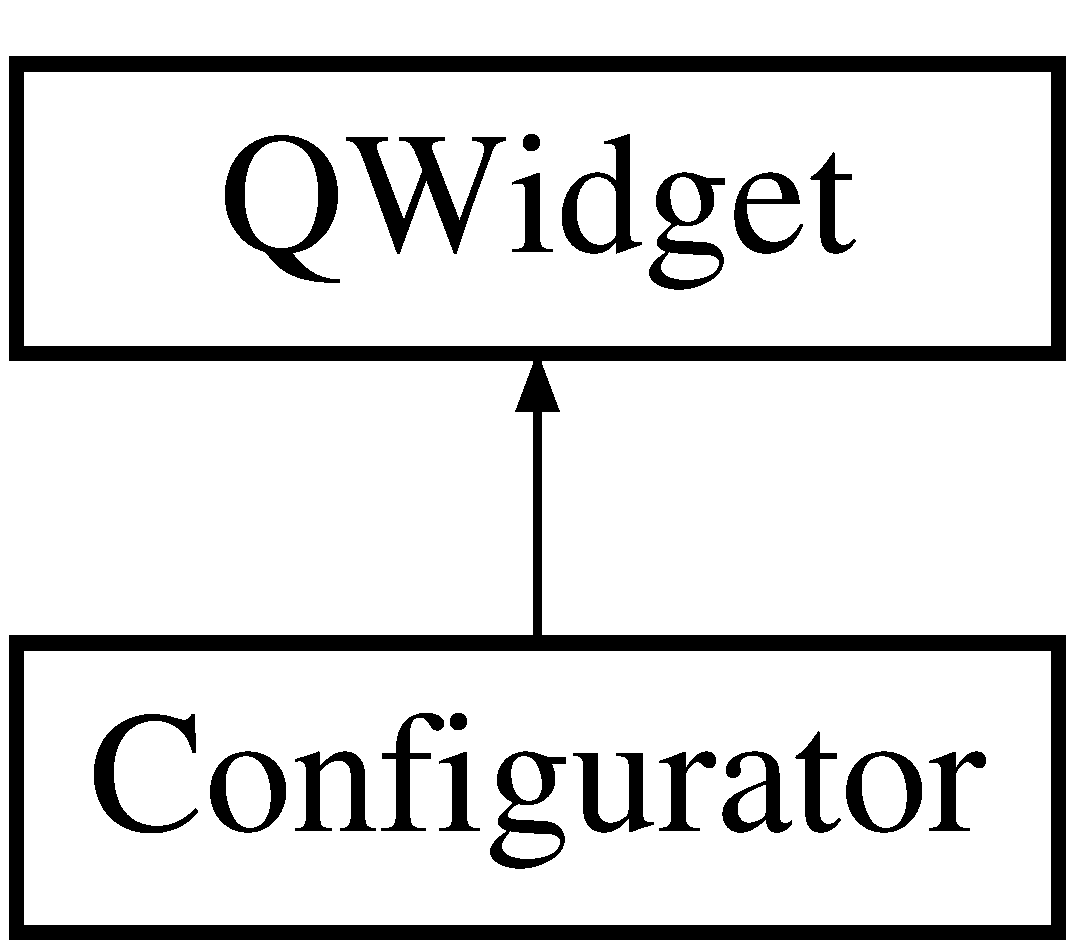
\includegraphics[height=2.000000cm]{class_configurator}
\end{center}
\end{figure}
\subsection*{Public Slots}
\begin{DoxyCompactItemize}
\item 
\mbox{\Hypertarget{class_configurator_a80a4e2988400839fe550f87fc3681cbb}\label{class_configurator_a80a4e2988400839fe550f87fc3681cbb}} 
void \mbox{\hyperlink{class_configurator_a80a4e2988400839fe550f87fc3681cbb}{on\+Confirm}} ()
\begin{DoxyCompactList}\small\item\em Slot connected to button press event. Emits the value\+Update signal. \end{DoxyCompactList}\end{DoxyCompactItemize}
\subsection*{Signals}
\begin{DoxyCompactItemize}
\item 
void \mbox{\hyperlink{class_configurator_ab558c7a35d9d766fe3a7ae80326223f0}{value\+Update}} (Q\+Json\+Object new\+\_\+values)
\begin{DoxyCompactList}\small\item\em Emits a signal that new values are available. \end{DoxyCompactList}\end{DoxyCompactItemize}
\subsection*{Public Member Functions}
\begin{DoxyCompactItemize}
\item 
\mbox{\Hypertarget{class_configurator_a7908b0494f0e057fc0b91c334d5902f9}\label{class_configurator_a7908b0494f0e057fc0b91c334d5902f9}} 
{\bfseries Configurator} (const Q\+Json\+Object \&config, Q\+Widget $\ast$parent=Q\+\_\+\+N\+U\+L\+L\+P\+TR)
\item 
Q\+Json\+Object \mbox{\hyperlink{class_configurator_a89fc398da91616473846cfcadd511c81}{get\+Values}} () const
\begin{DoxyCompactList}\small\item\em Returns the set values of all nested U\+I-\/elements as json object. \end{DoxyCompactList}\item 
void \mbox{\hyperlink{class_configurator_abb86d4cefc42b8e79fc440e2b13dd9d8}{set\+Values}} (const Q\+Json\+Object \&values)
\begin{DoxyCompactList}\small\item\em Set values from given json object. \end{DoxyCompactList}\end{DoxyCompactItemize}


\subsection{Detailed Description}
The \mbox{\hyperlink{class_configurator}{Configurator}} class creates a mondular user interfaces consisting of ui groups with Qt style spin boxes. 

A user interface configuraion file has the following basic layout, starting off with a $<$string$>$ specifying the Confirm buttons label, as well as an array containing groups of ui elements to be created.

\{ \char`\"{}confirm\+\_\+message\char`\"{} \+: \char`\"{}\+Recalculate\char`\"{}, \char`\"{}ui\char`\"{} \+: \mbox{[}...\mbox{]} \}

Each major group gets a title as well as a key attribute matching the key specified within the respective model configuration. The key is important for the main application to build a correspondence between user interface and model configuraion. Furthermore, to-\/be-\/created ui groups are given as attributes of a json object. This is done in order to maintain the order of groups specified in the json file within the application.

\{ \char`\"{}title\char`\"{}\+: \char`\"{}\+Projector\char`\"{}, \char`\"{}attribute\char`\"{}\+: \char`\"{}projector\char`\"{}, \char`\"{}groups\char`\"{}\+: \{ ... \}, \}

Groups are specified by simple creating a named json object. Containing a title, again another key to identify the attribute it changes. Important is, that the objects name as well as the string inclueded within the \textquotesingle{}attrbute\textquotesingle{} field M\+U\+ST match. Finally each group contains an array which specifies the amount of values to be captured. For each element of the \textquotesingle{}elements\textquotesingle{} array, the applicaion will create a simple Q\+Spinbox.

\{ \char`\"{}position\char`\"{}\+: \{ \char`\"{}title\char`\"{}\+: \char`\"{}\+Position\char`\"{}, \char`\"{}attribute\char`\"{} \+: \char`\"{}position\char`\"{}, \char`\"{}elements\char`\"{} \+: \mbox{[}...\mbox{]}, \}

Each Element to be created needs several attributes in order to function properly. First the Spinboxes title, as well as the attribute it captures. In addition to that the minimum, maximum and the precision need to be specified

\{ \char`\"{}title\char`\"{}\+: \char`\"{}\+X\char`\"{}, \char`\"{}attribute\char`\"{}\+: \char`\"{}x\char`\"{}, \char`\"{}precision\char`\"{}\+: 0.\+01, \char`\"{}min\char`\"{}\+: -\/2.\+0, \char`\"{}max\char`\"{}\+: 2.\+0 \}, 

\subsection{Member Function Documentation}
\mbox{\Hypertarget{class_configurator_a89fc398da91616473846cfcadd511c81}\label{class_configurator_a89fc398da91616473846cfcadd511c81}} 
\index{Configurator@{Configurator}!get\+Values@{get\+Values}}
\index{get\+Values@{get\+Values}!Configurator@{Configurator}}
\subsubsection{\texorpdfstring{get\+Values()}{getValues()}}
{\footnotesize\ttfamily Q\+Json\+Object Configurator\+::get\+Values (\begin{DoxyParamCaption}{ }\end{DoxyParamCaption}) const}



Returns the set values of all nested U\+I-\/elements as json object. 

\begin{DoxyReturn}{Returns}

\end{DoxyReturn}
\mbox{\Hypertarget{class_configurator_abb86d4cefc42b8e79fc440e2b13dd9d8}\label{class_configurator_abb86d4cefc42b8e79fc440e2b13dd9d8}} 
\index{Configurator@{Configurator}!set\+Values@{set\+Values}}
\index{set\+Values@{set\+Values}!Configurator@{Configurator}}
\subsubsection{\texorpdfstring{set\+Values()}{setValues()}}
{\footnotesize\ttfamily void Configurator\+::set\+Values (\begin{DoxyParamCaption}\item[{const Q\+Json\+Object \&}]{values }\end{DoxyParamCaption})}



Set values from given json object. 

Information on the json structure can be found at this classes main description $\ast$


\begin{DoxyParams}{Parameters}
{\em values} & specifies a json object containing information on which U\+I-\/element should be set to with the given value \\
\hline
\end{DoxyParams}
\mbox{\Hypertarget{class_configurator_ab558c7a35d9d766fe3a7ae80326223f0}\label{class_configurator_ab558c7a35d9d766fe3a7ae80326223f0}} 
\index{Configurator@{Configurator}!value\+Update@{value\+Update}}
\index{value\+Update@{value\+Update}!Configurator@{Configurator}}
\subsubsection{\texorpdfstring{value\+Update}{valueUpdate}}
{\footnotesize\ttfamily void Configurator\+::value\+Update (\begin{DoxyParamCaption}\item[{Q\+Json\+Object}]{new\+\_\+values }\end{DoxyParamCaption})\hspace{0.3cm}{\ttfamily [signal]}}



Emits a signal that new values are available. 


\begin{DoxyParams}{Parameters}
{\em new\+\_\+values} & \\
\hline
\end{DoxyParams}


The documentation for this class was generated from the following files\+:\begin{DoxyCompactItemize}
\item 
/\+Users/h\+Gen/\+Desktop/qt/glwarp-\/configuration-\/tool/src/ui/configurator.\+h\item 
/\+Users/h\+Gen/\+Desktop/qt/glwarp-\/configuration-\/tool/src/ui/configurator.\+cpp\end{DoxyCompactItemize}

\hypertarget{class_dome_projector}{}\section{Dome\+Projector Class Reference}
\label{class_dome_projector}\index{Dome\+Projector@{Dome\+Projector}}


The \mbox{\hyperlink{class_dome_projector}{Dome\+Projector}} class describes a projector specialized on calculating a warping geometry.  




{\ttfamily \#include $<$dome\+\_\+projector.\+hpp$>$}

\subsection*{Public Member Functions}
\begin{DoxyCompactItemize}
\item 
\mbox{\hyperlink{class_dome_projector_aea4bdc99173b4fcc44388d5efb204ceb}{Dome\+Projector}} (\mbox{\hyperlink{class_projector_frustum}{Projector\+Frustum}} $\ast$\+\_\+frustum, int \+\_\+grid\+\_\+rings, int \+\_\+grid\+\_\+ring\+\_\+elements, Q\+Vector3D const \&position, int dome\+\_\+rings, int dome\+\_\+ring\+\_\+elements)
\item 
\mbox{\hyperlink{class_dome_projector_aa4ae5284677524033bcafb09dcd132b2}{$\sim$\+Dome\+Projector}} ()
\item 
\mbox{\Hypertarget{class_dome_projector_a2fc9fff775752f59c2ff961f8696eba1}\label{class_dome_projector_a2fc9fff775752f59c2ff961f8696eba1}} 
void \mbox{\hyperlink{class_dome_projector_a2fc9fff775752f59c2ff961f8696eba1}{initialize}} ()
\begin{DoxyCompactList}\small\item\em initialize \end{DoxyCompactList}\item 
void \mbox{\hyperlink{class_dome_projector_a28963378c069176dc852605e02a12ed4}{calculate\+Transformation\+Mesh}} ()
\begin{DoxyCompactList}\small\item\em Calculates the transformation mesh using data previously simulated. \end{DoxyCompactList}\item 
void \mbox{\hyperlink{class_dome_projector_a1d8bd78cd24cbd92d6605b4cc3d061c3}{calculate\+Dome\+Hitpoints}} (\mbox{\hyperlink{class_sphere}{Sphere}} $\ast$mirror, \mbox{\hyperlink{class_sphere}{Sphere}} $\ast$dome)
\begin{DoxyCompactList}\small\item\em Performs a raycast, aiming to hit the dome using the mirror as reflection medium. \end{DoxyCompactList}\item 
void \mbox{\hyperlink{class_dome_projector_a70b4a39dec84fa11faf57a7dbd422c37}{update\+From\+Config}} (\mbox{\hyperlink{struct_model_config}{Model\+Config}} $\ast$model\+\_\+config)
\begin{DoxyCompactList}\small\item\em Updates internal values from given config. \end{DoxyCompactList}\item 
\mbox{\hyperlink{class_projector_frustum}{Projector\+Frustum}} $\ast$ \mbox{\hyperlink{class_dome_projector_a6d7a65d45ce490b25d79694ec2b76f3b}{get\+Frustum}} () const
\item 
void \mbox{\hyperlink{class_dome_projector_afd963b30b1cd4fa401de40ce99a5da7b}{translate}} (Q\+Vector3D position)
\begin{DoxyCompactList}\small\item\em Alter the \mbox{\hyperlink{class_dome_projector}{Dome\+Projector}}\textquotesingle{}s position. \end{DoxyCompactList}\item 
std\+::vector$<$ Q\+Vector3D $>$ \mbox{\hyperlink{class_dome_projector_a7289aa1fc872437e0ce0ced081f3ca87}{get\+Mesh\+Coords}} () const
\begin{DoxyCompactList}\small\item\em Returns calculated mesh coordinates. \end{DoxyCompactList}\item 
std\+::vector$<$ Q\+Vector3D $>$ \mbox{\hyperlink{class_dome_projector_abb4b7cda4a5e64e3069a1b5ace4a8ca2}{get\+Tex\+Coords}} () const
\begin{DoxyCompactList}\small\item\em Returns calculated texture coordinates. \end{DoxyCompactList}\end{DoxyCompactItemize}
\subsection*{Public Attributes}
\begin{DoxyCompactItemize}
\item 
\mbox{\Hypertarget{class_dome_projector_aee69ea0cbe641217af998cbb6669d91a}\label{class_dome_projector_aee69ea0cbe641217af998cbb6669d91a}} 
std\+::vector$<$ Q\+Vector3D $>$ {\bfseries sample\+\_\+grid}
\item 
\mbox{\Hypertarget{class_dome_projector_a5d157d37386f714b94dd04455019749b}\label{class_dome_projector_a5d157d37386f714b94dd04455019749b}} 
std\+::vector$<$ Q\+Vector3D $>$ {\bfseries first\+\_\+hits}
\item 
\mbox{\Hypertarget{class_dome_projector_aec6c5285b17e5c73537c45eb62bada81}\label{class_dome_projector_aec6c5285b17e5c73537c45eb62bada81}} 
std\+::vector$<$ Q\+Vector3D $>$ {\bfseries second\+\_\+hits}
\item 
\mbox{\Hypertarget{class_dome_projector_a65dad2376d52d0ec2601f4a797a3b4f2}\label{class_dome_projector_a65dad2376d52d0ec2601f4a797a3b4f2}} 
std\+::vector$<$ Q\+Vector3D $>$ {\bfseries dome\+\_\+vertices}
\item 
\mbox{\Hypertarget{class_dome_projector_aa1540ea0ff8e2211b20176f04adb5455}\label{class_dome_projector_aa1540ea0ff8e2211b20176f04adb5455}} 
std\+::vector$<$ Q\+Vector3D $>$ {\bfseries mesh\+\_\+coords}
\item 
\mbox{\Hypertarget{class_dome_projector_a28f75086f3ce94c35a3d6c7d102709db}\label{class_dome_projector_a28f75086f3ce94c35a3d6c7d102709db}} 
std\+::vector$<$ Q\+Vector3D $>$ {\bfseries texture\+\_\+coords}
\end{DoxyCompactItemize}


\subsection{Detailed Description}
The \mbox{\hyperlink{class_dome_projector}{Dome\+Projector}} class describes a projector specialized on calculating a warping geometry. 

The dome projector calculates a, for the given model accurate projection mesh. 

\subsection{Constructor \& Destructor Documentation}
\mbox{\Hypertarget{class_dome_projector_aea4bdc99173b4fcc44388d5efb204ceb}\label{class_dome_projector_aea4bdc99173b4fcc44388d5efb204ceb}} 
\index{Dome\+Projector@{Dome\+Projector}!Dome\+Projector@{Dome\+Projector}}
\index{Dome\+Projector@{Dome\+Projector}!Dome\+Projector@{Dome\+Projector}}
\subsubsection{\texorpdfstring{Dome\+Projector()}{DomeProjector()}}
{\footnotesize\ttfamily Dome\+Projector\+::\+Dome\+Projector (\begin{DoxyParamCaption}\item[{\mbox{\hyperlink{class_projector_frustum}{Projector\+Frustum}} $\ast$}]{\+\_\+frustum,  }\item[{int}]{\+\_\+grid\+\_\+rings,  }\item[{int}]{\+\_\+grid\+\_\+ring\+\_\+elements,  }\item[{Q\+Vector3D const \&}]{position,  }\item[{int}]{dome\+\_\+rings,  }\item[{int}]{dome\+\_\+ring\+\_\+elements }\end{DoxyParamCaption})}

Creates a dome projector object alongside the specified sample grid 
\begin{DoxyParams}{Parameters}
{\em \+\_\+frustum} & \\
\hline
{\em \+\_\+screen} & \\
\hline
{\em \+\_\+grid\+\_\+rings} & \\
\hline
{\em \+\_\+grid\+\_\+ring\+\_\+elements} & \\
\hline
\end{DoxyParams}
\mbox{\Hypertarget{class_dome_projector_aa4ae5284677524033bcafb09dcd132b2}\label{class_dome_projector_aa4ae5284677524033bcafb09dcd132b2}} 
\index{Dome\+Projector@{Dome\+Projector}!````~Dome\+Projector@{$\sim$\+Dome\+Projector}}
\index{````~Dome\+Projector@{$\sim$\+Dome\+Projector}!Dome\+Projector@{Dome\+Projector}}
\subsubsection{\texorpdfstring{$\sim$\+Dome\+Projector()}{~DomeProjector()}}
{\footnotesize\ttfamily Dome\+Projector\+::$\sim$\+Dome\+Projector (\begin{DoxyParamCaption}{ }\end{DoxyParamCaption})}

Destructor 

\subsection{Member Function Documentation}
\mbox{\Hypertarget{class_dome_projector_a1d8bd78cd24cbd92d6605b4cc3d061c3}\label{class_dome_projector_a1d8bd78cd24cbd92d6605b4cc3d061c3}} 
\index{Dome\+Projector@{Dome\+Projector}!calculate\+Dome\+Hitpoints@{calculate\+Dome\+Hitpoints}}
\index{calculate\+Dome\+Hitpoints@{calculate\+Dome\+Hitpoints}!Dome\+Projector@{Dome\+Projector}}
\subsubsection{\texorpdfstring{calculate\+Dome\+Hitpoints()}{calculateDomeHitpoints()}}
{\footnotesize\ttfamily void Dome\+Projector\+::calculate\+Dome\+Hitpoints (\begin{DoxyParamCaption}\item[{\mbox{\hyperlink{class_sphere}{Sphere}} $\ast$}]{mirror,  }\item[{\mbox{\hyperlink{class_sphere}{Sphere}} $\ast$}]{dome }\end{DoxyParamCaption})}



Performs a raycast, aiming to hit the dome using the mirror as reflection medium. 


\begin{DoxyParams}{Parameters}
{\em mirror} & \\
\hline
{\em dome} & \\
\hline
\end{DoxyParams}
\mbox{\Hypertarget{class_dome_projector_a28963378c069176dc852605e02a12ed4}\label{class_dome_projector_a28963378c069176dc852605e02a12ed4}} 
\index{Dome\+Projector@{Dome\+Projector}!calculate\+Transformation\+Mesh@{calculate\+Transformation\+Mesh}}
\index{calculate\+Transformation\+Mesh@{calculate\+Transformation\+Mesh}!Dome\+Projector@{Dome\+Projector}}
\subsubsection{\texorpdfstring{calculate\+Transformation\+Mesh()}{calculateTransformationMesh()}}
{\footnotesize\ttfamily void Dome\+Projector\+::calculate\+Transformation\+Mesh (\begin{DoxyParamCaption}{ }\end{DoxyParamCaption})}



Calculates the transformation mesh using data previously simulated. 

\begin{DoxyReturn}{Returns}
std\+::vector$<$\+Q\+Vector3\+D$>$ transformation mesh 
\end{DoxyReturn}
\mbox{\Hypertarget{class_dome_projector_a6d7a65d45ce490b25d79694ec2b76f3b}\label{class_dome_projector_a6d7a65d45ce490b25d79694ec2b76f3b}} 
\index{Dome\+Projector@{Dome\+Projector}!get\+Frustum@{get\+Frustum}}
\index{get\+Frustum@{get\+Frustum}!Dome\+Projector@{Dome\+Projector}}
\subsubsection{\texorpdfstring{get\+Frustum()}{getFrustum()}}
{\footnotesize\ttfamily \mbox{\hyperlink{class_projector_frustum}{Projector\+Frustum}} $\ast$ Dome\+Projector\+::get\+Frustum (\begin{DoxyParamCaption}{ }\end{DoxyParamCaption}) const}

Returns the projectors frustum. \begin{DoxyReturn}{Returns}

\end{DoxyReturn}
\mbox{\Hypertarget{class_dome_projector_a7289aa1fc872437e0ce0ced081f3ca87}\label{class_dome_projector_a7289aa1fc872437e0ce0ced081f3ca87}} 
\index{Dome\+Projector@{Dome\+Projector}!get\+Mesh\+Coords@{get\+Mesh\+Coords}}
\index{get\+Mesh\+Coords@{get\+Mesh\+Coords}!Dome\+Projector@{Dome\+Projector}}
\subsubsection{\texorpdfstring{get\+Mesh\+Coords()}{getMeshCoords()}}
{\footnotesize\ttfamily std\+::vector$<$ Q\+Vector3D $>$ Dome\+Projector\+::get\+Mesh\+Coords (\begin{DoxyParamCaption}{ }\end{DoxyParamCaption}) const}



Returns calculated mesh coordinates. 

\begin{DoxyReturn}{Returns}

\end{DoxyReturn}
\mbox{\Hypertarget{class_dome_projector_abb4b7cda4a5e64e3069a1b5ace4a8ca2}\label{class_dome_projector_abb4b7cda4a5e64e3069a1b5ace4a8ca2}} 
\index{Dome\+Projector@{Dome\+Projector}!get\+Tex\+Coords@{get\+Tex\+Coords}}
\index{get\+Tex\+Coords@{get\+Tex\+Coords}!Dome\+Projector@{Dome\+Projector}}
\subsubsection{\texorpdfstring{get\+Tex\+Coords()}{getTexCoords()}}
{\footnotesize\ttfamily std\+::vector$<$ Q\+Vector3D $>$ Dome\+Projector\+::get\+Tex\+Coords (\begin{DoxyParamCaption}{ }\end{DoxyParamCaption}) const}



Returns calculated texture coordinates. 

\begin{DoxyReturn}{Returns}

\end{DoxyReturn}
\mbox{\Hypertarget{class_dome_projector_afd963b30b1cd4fa401de40ce99a5da7b}\label{class_dome_projector_afd963b30b1cd4fa401de40ce99a5da7b}} 
\index{Dome\+Projector@{Dome\+Projector}!translate@{translate}}
\index{translate@{translate}!Dome\+Projector@{Dome\+Projector}}
\subsubsection{\texorpdfstring{translate()}{translate()}}
{\footnotesize\ttfamily void Dome\+Projector\+::translate (\begin{DoxyParamCaption}\item[{Q\+Vector3D}]{position }\end{DoxyParamCaption})}



Alter the \mbox{\hyperlink{class_dome_projector}{Dome\+Projector}}\textquotesingle{}s position. 


\begin{DoxyParams}{Parameters}
{\em position} & \\
\hline
\end{DoxyParams}
\mbox{\Hypertarget{class_dome_projector_a70b4a39dec84fa11faf57a7dbd422c37}\label{class_dome_projector_a70b4a39dec84fa11faf57a7dbd422c37}} 
\index{Dome\+Projector@{Dome\+Projector}!update\+From\+Config@{update\+From\+Config}}
\index{update\+From\+Config@{update\+From\+Config}!Dome\+Projector@{Dome\+Projector}}
\subsubsection{\texorpdfstring{update\+From\+Config()}{updateFromConfig()}}
{\footnotesize\ttfamily void Dome\+Projector\+::update\+From\+Config (\begin{DoxyParamCaption}\item[{\mbox{\hyperlink{struct_model_config}{Model\+Config}} $\ast$}]{model\+\_\+config }\end{DoxyParamCaption})}



Updates internal values from given config. 

It thereby regenerates the radial sampling grid as well as the dome grid with the specified values. 
\begin{DoxyParams}{Parameters}
{\em model\+\_\+config} & \\
\hline
\end{DoxyParams}


The documentation for this class was generated from the following files\+:\begin{DoxyCompactItemize}
\item 
/\+Users/h\+Gen/\+Desktop/qt/glwarp-\/configuration-\/tool/src/model/dome\+\_\+projector.\+hpp\item 
/\+Users/h\+Gen/\+Desktop/qt/glwarp-\/configuration-\/tool/src/model/dome\+\_\+projector.\+cpp\end{DoxyCompactItemize}

\hypertarget{struct_dome_projector_config}{}\section{Dome\+Projector\+Config Struct Reference}
\label{struct_dome_projector_config}\index{Dome\+Projector\+Config@{Dome\+Projector\+Config}}
\subsection*{Static Public Member Functions}
\begin{DoxyCompactItemize}
\item 
\mbox{\Hypertarget{struct_dome_projector_config_a7bf2620a0e55675ce701d53b6e64b358}\label{struct_dome_projector_config_a7bf2620a0e55675ce701d53b6e64b358}} 
static \mbox{\hyperlink{struct_dome_projector_config}{Dome\+Projector\+Config}} {\bfseries from\+Json} (const Q\+Json\+Object \&object)
\end{DoxyCompactItemize}
\subsection*{Public Attributes}
\begin{DoxyCompactItemize}
\item 
\mbox{\Hypertarget{struct_dome_projector_config_af5c5dd95ae20706d1fcf4d6a127cb7ab}\label{struct_dome_projector_config_af5c5dd95ae20706d1fcf4d6a127cb7ab}} 
Q\+Vector3D {\bfseries position}
\item 
\mbox{\Hypertarget{struct_dome_projector_config_ad5a86b3c2b1cf2483f4439f543c29d40}\label{struct_dome_projector_config_ad5a86b3c2b1cf2483f4439f543c29d40}} 
Q\+Vector3D {\bfseries rotation}
\item 
\mbox{\Hypertarget{struct_dome_projector_config_a036a018d258a937798f75250d5fc5efd}\label{struct_dome_projector_config_a036a018d258a937798f75250d5fc5efd}} 
float {\bfseries fov}
\item 
\mbox{\Hypertarget{struct_dome_projector_config_aefb4e3ec8b8cd2899791e7260eece342}\label{struct_dome_projector_config_aefb4e3ec8b8cd2899791e7260eece342}} 
int {\bfseries screen\+\_\+width}
\item 
\mbox{\Hypertarget{struct_dome_projector_config_a18b6efba3fdecacb70a2a452fb83d137}\label{struct_dome_projector_config_a18b6efba3fdecacb70a2a452fb83d137}} 
int {\bfseries screen\+\_\+height}
\item 
\mbox{\Hypertarget{struct_dome_projector_config_a4a571d42c0e027764e1ed29b7e7a4981}\label{struct_dome_projector_config_a4a571d42c0e027764e1ed29b7e7a4981}} 
int {\bfseries num\+\_\+grid\+\_\+rings}
\item 
\mbox{\Hypertarget{struct_dome_projector_config_a9fed455ab623d8a23fe9b6c0f4657d7f}\label{struct_dome_projector_config_a9fed455ab623d8a23fe9b6c0f4657d7f}} 
int {\bfseries num\+\_\+grid\+\_\+ring\+\_\+elements}
\item 
\mbox{\Hypertarget{struct_dome_projector_config_aea8bf159f1e43b10fca1e25d9db2ec5b}\label{struct_dome_projector_config_aea8bf159f1e43b10fca1e25d9db2ec5b}} 
int {\bfseries num\+\_\+mesh\+\_\+rings}
\item 
\mbox{\Hypertarget{struct_dome_projector_config_aab153e6f541c89b2130022ea2f79ab0b}\label{struct_dome_projector_config_aab153e6f541c89b2130022ea2f79ab0b}} 
int {\bfseries num\+\_\+mesh\+\_\+ring\+\_\+elements}
\end{DoxyCompactItemize}


The documentation for this struct was generated from the following files\+:\begin{DoxyCompactItemize}
\item 
/\+Users/h\+Gen/\+Desktop/qt/glwarp-\/configuration-\/tool/src/config.\+h\item 
/\+Users/h\+Gen/\+Desktop/qt/glwarp-\/configuration-\/tool/src/config.\+cpp\end{DoxyCompactItemize}

\hypertarget{class_g_l_warp_widget}{}\section{G\+L\+Warp\+Widget Class Reference}
\label{class_g_l_warp_widget}\index{G\+L\+Warp\+Widget@{G\+L\+Warp\+Widget}}
Inheritance diagram for G\+L\+Warp\+Widget\+:\begin{figure}[H]
\begin{center}
\leavevmode
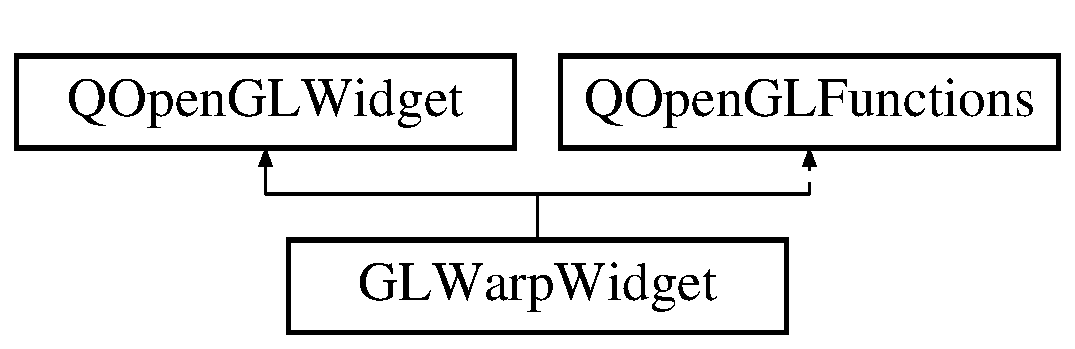
\includegraphics[height=2.000000cm]{class_g_l_warp_widget}
\end{center}
\end{figure}
\subsection*{Public Slots}
\begin{DoxyCompactItemize}
\item 
\mbox{\Hypertarget{class_g_l_warp_widget_a24e35ffcefc3499ec94c1e233d9f1b22}\label{class_g_l_warp_widget_a24e35ffcefc3499ec94c1e233d9f1b22}} 
void {\bfseries cleanup} ()
\item 
\mbox{\Hypertarget{class_g_l_warp_widget_a5de5b6170929ad43973d9156c6c577d1}\label{class_g_l_warp_widget_a5de5b6170929ad43973d9156c6c577d1}} 
void {\bfseries key\+Press\+Event} (Q\+Key\+Event $\ast$event) override
\end{DoxyCompactItemize}
\subsection*{Public Member Functions}
\begin{DoxyCompactItemize}
\item 
\mbox{\hyperlink{class_g_l_warp_widget_a5b2cdeb05b78d1acb1f13e59a691a001}{G\+L\+Warp\+Widget}} (Q\+Widget $\ast$parent=Q\+\_\+\+N\+U\+L\+L\+P\+TR)
\begin{DoxyCompactList}\small\item\em \mbox{\hyperlink{class_g_l_widget}{G\+L\+Widget}}. \end{DoxyCompactList}\item 
\mbox{\hyperlink{class_g_l_warp_widget_a38b3a090564985953d31003630985361}{$\sim$\+G\+L\+Warp\+Widget}} ()
\item 
Q\+Size \mbox{\hyperlink{class_g_l_warp_widget_aee1b83d5cce73680d18b10432834dbcc}{minimum\+Size\+Hint}} () const override
\begin{DoxyCompactList}\small\item\em minimum\+Size\+Hint \end{DoxyCompactList}\item 
Q\+Size \mbox{\hyperlink{class_g_l_warp_widget_ab48f61235afc35cfac013edb34445c57}{size\+Hint}} () const override
\begin{DoxyCompactList}\small\item\em size\+Hint \end{DoxyCompactList}\item 
void \mbox{\hyperlink{class_g_l_warp_widget_ac7619517a9aa914452fa39092242b3b3}{update\+Values}} (std\+::vector$<$ Q\+Vector3D $>$ mesh\+\_\+values, std\+::vector$<$ Q\+Vector3D $>$ uv\+\_\+values)
\begin{DoxyCompactList}\small\item\em Update the mesh and uv\+\_\+values. \end{DoxyCompactList}\end{DoxyCompactItemize}
\subsection*{Protected Member Functions}
\begin{DoxyCompactItemize}
\item 
\mbox{\Hypertarget{class_g_l_warp_widget_ae5168c23c1d80794c85cc3401c5fbf91}\label{class_g_l_warp_widget_ae5168c23c1d80794c85cc3401c5fbf91}} 
void \mbox{\hyperlink{class_g_l_warp_widget_ae5168c23c1d80794c85cc3401c5fbf91}{initialize\+GL}} () override
\begin{DoxyCompactList}\small\item\em Initializes the Qt-\/\+Open\+GL context. \end{DoxyCompactList}\item 
\mbox{\Hypertarget{class_g_l_warp_widget_a970521ed7331e205962fd3b669234980}\label{class_g_l_warp_widget_a970521ed7331e205962fd3b669234980}} 
void \mbox{\hyperlink{class_g_l_warp_widget_a970521ed7331e205962fd3b669234980}{paint\+GL}} () override
\begin{DoxyCompactList}\small\item\em paint\+GL \end{DoxyCompactList}\item 
void \mbox{\hyperlink{class_g_l_warp_widget_a3f5becb91977e33d64f40ad68c903b64}{resize\+GL}} (int width, int height) override
\begin{DoxyCompactList}\small\item\em resize\+GL \end{DoxyCompactList}\end{DoxyCompactItemize}


\subsection{Constructor \& Destructor Documentation}
\mbox{\Hypertarget{class_g_l_warp_widget_a5b2cdeb05b78d1acb1f13e59a691a001}\label{class_g_l_warp_widget_a5b2cdeb05b78d1acb1f13e59a691a001}} 
\index{G\+L\+Warp\+Widget@{G\+L\+Warp\+Widget}!G\+L\+Warp\+Widget@{G\+L\+Warp\+Widget}}
\index{G\+L\+Warp\+Widget@{G\+L\+Warp\+Widget}!G\+L\+Warp\+Widget@{G\+L\+Warp\+Widget}}
\subsubsection{\texorpdfstring{G\+L\+Warp\+Widget()}{GLWarpWidget()}}
{\footnotesize\ttfamily G\+L\+Warp\+Widget\+::\+G\+L\+Warp\+Widget (\begin{DoxyParamCaption}\item[{Q\+Widget $\ast$}]{parent = {\ttfamily Q\+\_\+NULLPTR} }\end{DoxyParamCaption})}



\mbox{\hyperlink{class_g_l_widget}{G\+L\+Widget}}. 


\begin{DoxyParams}{Parameters}
{\em parent} & \\
\hline
\end{DoxyParams}
\mbox{\Hypertarget{class_g_l_warp_widget_a38b3a090564985953d31003630985361}\label{class_g_l_warp_widget_a38b3a090564985953d31003630985361}} 
\index{G\+L\+Warp\+Widget@{G\+L\+Warp\+Widget}!````~G\+L\+Warp\+Widget@{$\sim$\+G\+L\+Warp\+Widget}}
\index{````~G\+L\+Warp\+Widget@{$\sim$\+G\+L\+Warp\+Widget}!G\+L\+Warp\+Widget@{G\+L\+Warp\+Widget}}
\subsubsection{\texorpdfstring{$\sim$\+G\+L\+Warp\+Widget()}{~GLWarpWidget()}}
{\footnotesize\ttfamily G\+L\+Warp\+Widget\+::$\sim$\+G\+L\+Warp\+Widget (\begin{DoxyParamCaption}{ }\end{DoxyParamCaption})}

d\textquotesingle{}tor 

\subsection{Member Function Documentation}
\mbox{\Hypertarget{class_g_l_warp_widget_aee1b83d5cce73680d18b10432834dbcc}\label{class_g_l_warp_widget_aee1b83d5cce73680d18b10432834dbcc}} 
\index{G\+L\+Warp\+Widget@{G\+L\+Warp\+Widget}!minimum\+Size\+Hint@{minimum\+Size\+Hint}}
\index{minimum\+Size\+Hint@{minimum\+Size\+Hint}!G\+L\+Warp\+Widget@{G\+L\+Warp\+Widget}}
\subsubsection{\texorpdfstring{minimum\+Size\+Hint()}{minimumSizeHint()}}
{\footnotesize\ttfamily Q\+Size G\+L\+Warp\+Widget\+::minimum\+Size\+Hint (\begin{DoxyParamCaption}{ }\end{DoxyParamCaption}) const\hspace{0.3cm}{\ttfamily [override]}}



minimum\+Size\+Hint 

\begin{DoxyReturn}{Returns}

\end{DoxyReturn}
\mbox{\Hypertarget{class_g_l_warp_widget_a3f5becb91977e33d64f40ad68c903b64}\label{class_g_l_warp_widget_a3f5becb91977e33d64f40ad68c903b64}} 
\index{G\+L\+Warp\+Widget@{G\+L\+Warp\+Widget}!resize\+GL@{resize\+GL}}
\index{resize\+GL@{resize\+GL}!G\+L\+Warp\+Widget@{G\+L\+Warp\+Widget}}
\subsubsection{\texorpdfstring{resize\+G\+L()}{resizeGL()}}
{\footnotesize\ttfamily void G\+L\+Warp\+Widget\+::resize\+GL (\begin{DoxyParamCaption}\item[{int}]{width,  }\item[{int}]{height }\end{DoxyParamCaption})\hspace{0.3cm}{\ttfamily [override]}, {\ttfamily [protected]}}



resize\+GL 


\begin{DoxyParams}{Parameters}
{\em width} & \\
\hline
{\em height} & \\
\hline
\end{DoxyParams}
\mbox{\Hypertarget{class_g_l_warp_widget_ab48f61235afc35cfac013edb34445c57}\label{class_g_l_warp_widget_ab48f61235afc35cfac013edb34445c57}} 
\index{G\+L\+Warp\+Widget@{G\+L\+Warp\+Widget}!size\+Hint@{size\+Hint}}
\index{size\+Hint@{size\+Hint}!G\+L\+Warp\+Widget@{G\+L\+Warp\+Widget}}
\subsubsection{\texorpdfstring{size\+Hint()}{sizeHint()}}
{\footnotesize\ttfamily Q\+Size G\+L\+Warp\+Widget\+::size\+Hint (\begin{DoxyParamCaption}{ }\end{DoxyParamCaption}) const\hspace{0.3cm}{\ttfamily [override]}}



size\+Hint 

\begin{DoxyReturn}{Returns}

\end{DoxyReturn}
\mbox{\Hypertarget{class_g_l_warp_widget_ac7619517a9aa914452fa39092242b3b3}\label{class_g_l_warp_widget_ac7619517a9aa914452fa39092242b3b3}} 
\index{G\+L\+Warp\+Widget@{G\+L\+Warp\+Widget}!update\+Values@{update\+Values}}
\index{update\+Values@{update\+Values}!G\+L\+Warp\+Widget@{G\+L\+Warp\+Widget}}
\subsubsection{\texorpdfstring{update\+Values()}{updateValues()}}
{\footnotesize\ttfamily void G\+L\+Warp\+Widget\+::update\+Values (\begin{DoxyParamCaption}\item[{std\+::vector$<$ Q\+Vector3D $>$}]{mesh\+\_\+values,  }\item[{std\+::vector$<$ Q\+Vector3D $>$}]{uv\+\_\+values }\end{DoxyParamCaption})}



Update the mesh and uv\+\_\+values. 


\begin{DoxyParams}{Parameters}
{\em mesh\+\_\+values} & \\
\hline
{\em uv\+\_\+values} & \\
\hline
\end{DoxyParams}


The documentation for this class was generated from the following files\+:\begin{DoxyCompactItemize}
\item 
/\+Users/h\+Gen/\+Desktop/qt/glwarp-\/configuration-\/tool/src/ui/glwarpwidget.\+h\item 
/\+Users/h\+Gen/\+Desktop/qt/glwarp-\/configuration-\/tool/src/ui/glwarpwidget.\+cpp\end{DoxyCompactItemize}

\hypertarget{class_g_l_widget}{}\section{G\+L\+Widget Class Reference}
\label{class_g_l_widget}\index{G\+L\+Widget@{G\+L\+Widget}}
Inheritance diagram for G\+L\+Widget\+:\begin{figure}[H]
\begin{center}
\leavevmode
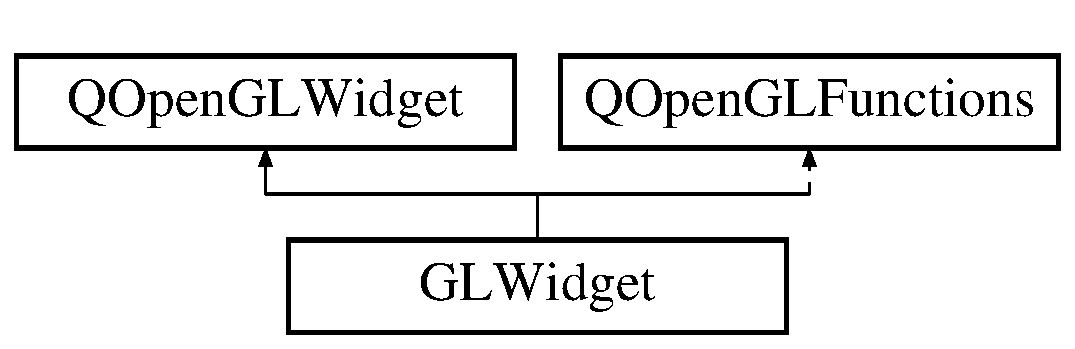
\includegraphics[height=2.000000cm]{class_g_l_widget}
\end{center}
\end{figure}
\subsection*{Public Slots}
\begin{DoxyCompactItemize}
\item 
\mbox{\Hypertarget{class_g_l_widget_a84c5673c0e92eac927220d368c505c94}\label{class_g_l_widget_a84c5673c0e92eac927220d368c505c94}} 
void {\bfseries cleanup} ()
\end{DoxyCompactItemize}
\subsection*{Signals}
\begin{DoxyCompactItemize}
\item 
void \mbox{\hyperlink{class_g_l_widget_a75a7f63bf253007d7dcbeee402e963d1}{update\+Scene}} (\mbox{\hyperlink{class_scene}{Scene}} scene)
\begin{DoxyCompactList}\small\item\em Updates the scene. \end{DoxyCompactList}\end{DoxyCompactItemize}
\subsection*{Public Member Functions}
\begin{DoxyCompactItemize}
\item 
\mbox{\Hypertarget{class_g_l_widget_a39ef1736aef8b1c6e2f7cff20b7a3997}\label{class_g_l_widget_a39ef1736aef8b1c6e2f7cff20b7a3997}} 
{\bfseries G\+L\+Widget} (Q\+Widget $\ast$parent=Q\+\_\+\+N\+U\+L\+L\+P\+TR)
\item 
Q\+Size \mbox{\hyperlink{class_g_l_widget_a1e50c746ef5d95c14de5907be6239dd1}{minimum\+Size\+Hint}} () const override
\begin{DoxyCompactList}\small\item\em minimum\+Size\+Hint \end{DoxyCompactList}\item 
Q\+Size \mbox{\hyperlink{class_g_l_widget_af04a97931fb78d610e1c73d7c4887319}{size\+Hint}} () const override
\begin{DoxyCompactList}\small\item\em size\+Hint \end{DoxyCompactList}\item 
void \mbox{\hyperlink{class_g_l_widget_ae31adda78d396b83f0891b8cde79a6cf}{set\+Scene}} (\mbox{\hyperlink{class_scene}{Scene}} scene)
\begin{DoxyCompactList}\small\item\em Sets the current scene. \end{DoxyCompactList}\end{DoxyCompactItemize}
\subsection*{Protected Member Functions}
\begin{DoxyCompactItemize}
\item 
\mbox{\Hypertarget{class_g_l_widget_a2349a3ff7c9cc814de1b4a93a0b28acd}\label{class_g_l_widget_a2349a3ff7c9cc814de1b4a93a0b28acd}} 
void \mbox{\hyperlink{class_g_l_widget_a2349a3ff7c9cc814de1b4a93a0b28acd}{initialize\+GL}} () override
\begin{DoxyCompactList}\small\item\em Initialize Open\+GL context. \end{DoxyCompactList}\item 
\mbox{\Hypertarget{class_g_l_widget_a843150d06edc5e2e50d98e395c2b8759}\label{class_g_l_widget_a843150d06edc5e2e50d98e395c2b8759}} 
void \mbox{\hyperlink{class_g_l_widget_a843150d06edc5e2e50d98e395c2b8759}{paint\+GL}} () override
\begin{DoxyCompactList}\small\item\em paint\+GL \end{DoxyCompactList}\item 
void \mbox{\hyperlink{class_g_l_widget_a71942bbb513fac0a1d4f0c1c24b37def}{resize\+GL}} (int width, int height) override
\begin{DoxyCompactList}\small\item\em resize\+GL \end{DoxyCompactList}\item 
\mbox{\Hypertarget{class_g_l_widget_afeba4699aa12cde94ecd469e58a60aab}\label{class_g_l_widget_afeba4699aa12cde94ecd469e58a60aab}} 
void {\bfseries mouse\+Press\+Event} (Q\+Mouse\+Event $\ast$event) override
\item 
\mbox{\Hypertarget{class_g_l_widget_a7cb45e554d24c2020512aa18949a6230}\label{class_g_l_widget_a7cb45e554d24c2020512aa18949a6230}} 
void {\bfseries mouse\+Move\+Event} (Q\+Mouse\+Event $\ast$event) override
\end{DoxyCompactItemize}


\subsection{Member Function Documentation}
\mbox{\Hypertarget{class_g_l_widget_a1e50c746ef5d95c14de5907be6239dd1}\label{class_g_l_widget_a1e50c746ef5d95c14de5907be6239dd1}} 
\index{G\+L\+Widget@{G\+L\+Widget}!minimum\+Size\+Hint@{minimum\+Size\+Hint}}
\index{minimum\+Size\+Hint@{minimum\+Size\+Hint}!G\+L\+Widget@{G\+L\+Widget}}
\subsubsection{\texorpdfstring{minimum\+Size\+Hint()}{minimumSizeHint()}}
{\footnotesize\ttfamily Q\+Size G\+L\+Widget\+::minimum\+Size\+Hint (\begin{DoxyParamCaption}{ }\end{DoxyParamCaption}) const\hspace{0.3cm}{\ttfamily [override]}}



minimum\+Size\+Hint 

\begin{DoxyReturn}{Returns}

\end{DoxyReturn}
\mbox{\Hypertarget{class_g_l_widget_a71942bbb513fac0a1d4f0c1c24b37def}\label{class_g_l_widget_a71942bbb513fac0a1d4f0c1c24b37def}} 
\index{G\+L\+Widget@{G\+L\+Widget}!resize\+GL@{resize\+GL}}
\index{resize\+GL@{resize\+GL}!G\+L\+Widget@{G\+L\+Widget}}
\subsubsection{\texorpdfstring{resize\+G\+L()}{resizeGL()}}
{\footnotesize\ttfamily void G\+L\+Widget\+::resize\+GL (\begin{DoxyParamCaption}\item[{int}]{width,  }\item[{int}]{height }\end{DoxyParamCaption})\hspace{0.3cm}{\ttfamily [override]}, {\ttfamily [protected]}}



resize\+GL 


\begin{DoxyParams}{Parameters}
{\em width} & \\
\hline
{\em height} & \\
\hline
\end{DoxyParams}
\mbox{\Hypertarget{class_g_l_widget_ae31adda78d396b83f0891b8cde79a6cf}\label{class_g_l_widget_ae31adda78d396b83f0891b8cde79a6cf}} 
\index{G\+L\+Widget@{G\+L\+Widget}!set\+Scene@{set\+Scene}}
\index{set\+Scene@{set\+Scene}!G\+L\+Widget@{G\+L\+Widget}}
\subsubsection{\texorpdfstring{set\+Scene()}{setScene()}}
{\footnotesize\ttfamily void G\+L\+Widget\+::set\+Scene (\begin{DoxyParamCaption}\item[{\mbox{\hyperlink{class_scene}{Scene}}}]{scene }\end{DoxyParamCaption})}



Sets the current scene. 


\begin{DoxyParams}{Parameters}
{\em scene} & \\
\hline
\end{DoxyParams}
\mbox{\Hypertarget{class_g_l_widget_af04a97931fb78d610e1c73d7c4887319}\label{class_g_l_widget_af04a97931fb78d610e1c73d7c4887319}} 
\index{G\+L\+Widget@{G\+L\+Widget}!size\+Hint@{size\+Hint}}
\index{size\+Hint@{size\+Hint}!G\+L\+Widget@{G\+L\+Widget}}
\subsubsection{\texorpdfstring{size\+Hint()}{sizeHint()}}
{\footnotesize\ttfamily Q\+Size G\+L\+Widget\+::size\+Hint (\begin{DoxyParamCaption}{ }\end{DoxyParamCaption}) const\hspace{0.3cm}{\ttfamily [override]}}



size\+Hint 

\begin{DoxyReturn}{Returns}

\end{DoxyReturn}
\mbox{\Hypertarget{class_g_l_widget_a75a7f63bf253007d7dcbeee402e963d1}\label{class_g_l_widget_a75a7f63bf253007d7dcbeee402e963d1}} 
\index{G\+L\+Widget@{G\+L\+Widget}!update\+Scene@{update\+Scene}}
\index{update\+Scene@{update\+Scene}!G\+L\+Widget@{G\+L\+Widget}}
\subsubsection{\texorpdfstring{update\+Scene}{updateScene}}
{\footnotesize\ttfamily void G\+L\+Widget\+::update\+Scene (\begin{DoxyParamCaption}\item[{\mbox{\hyperlink{class_scene}{Scene}}}]{scene }\end{DoxyParamCaption})\hspace{0.3cm}{\ttfamily [signal]}}



Updates the scene. 


\begin{DoxyParams}{Parameters}
{\em scene} & \\
\hline
\end{DoxyParams}


The documentation for this class was generated from the following files\+:\begin{DoxyCompactItemize}
\item 
/\+Users/h\+Gen/\+Desktop/qt/glwarp-\/configuration-\/tool/src/ui/glwidget.\+h\item 
/\+Users/h\+Gen/\+Desktop/qt/glwarp-\/configuration-\/tool/src/ui/glwidget.\+cpp\end{DoxyCompactItemize}

\hypertarget{struct_hitpoint}{}\section{Hitpoint Struct Reference}
\label{struct_hitpoint}\index{Hitpoint@{Hitpoint}}


The \mbox{\hyperlink{struct_hitpoint}{Hitpoint}} struct contains the two hitpoints of a ray with volume.  




{\ttfamily \#include $<$hitpoint.\+hpp$>$}

\subsection*{Public Member Functions}
\begin{DoxyCompactItemize}
\item 
\mbox{\Hypertarget{struct_hitpoint_a8bccb7ee01b77bdefba3e37f11b8e8b7}\label{struct_hitpoint_a8bccb7ee01b77bdefba3e37f11b8e8b7}} 
\mbox{\hyperlink{struct_hitpoint_a8bccb7ee01b77bdefba3e37f11b8e8b7}{Hitpoint}} ()
\begin{DoxyCompactList}\small\item\em \mbox{\hyperlink{struct_hitpoint}{Hitpoint}}. \end{DoxyCompactList}\item 
\mbox{\hyperlink{struct_hitpoint_a544329fb8b4556202074ff60f941a1cc}{Hitpoint}} (const Q\+Vector3D \&position)
\begin{DoxyCompactList}\small\item\em \mbox{\hyperlink{struct_hitpoint}{Hitpoint}}. \end{DoxyCompactList}\item 
\mbox{\hyperlink{struct_hitpoint_a7f098fb5a60e88c5f0ff5ce1d3161b84}{Hitpoint}} (const Q\+Vector3D \&position, const Q\+Vector3D \&normal, double t)
\begin{DoxyCompactList}\small\item\em \mbox{\hyperlink{struct_hitpoint}{Hitpoint}}. \end{DoxyCompactList}\end{DoxyCompactItemize}
\subsection*{Public Attributes}
\begin{DoxyCompactItemize}
\item 
\mbox{\Hypertarget{struct_hitpoint_ab843d522bc585010bd61715feba760ba}\label{struct_hitpoint_ab843d522bc585010bd61715feba760ba}} 
Q\+Vector3D {\bfseries position}
\item 
\mbox{\Hypertarget{struct_hitpoint_aaea463dd226da74d5c5d730409b77509}\label{struct_hitpoint_aaea463dd226da74d5c5d730409b77509}} 
Q\+Vector3D {\bfseries normal}
\item 
\mbox{\Hypertarget{struct_hitpoint_a794dfaeecbe50280b13af9171b335abe}\label{struct_hitpoint_a794dfaeecbe50280b13af9171b335abe}} 
double {\bfseries t}
\end{DoxyCompactItemize}


\subsection{Detailed Description}
The \mbox{\hyperlink{struct_hitpoint}{Hitpoint}} struct contains the two hitpoints of a ray with volume. 

\subsection{Constructor \& Destructor Documentation}
\mbox{\Hypertarget{struct_hitpoint_a544329fb8b4556202074ff60f941a1cc}\label{struct_hitpoint_a544329fb8b4556202074ff60f941a1cc}} 
\index{Hitpoint@{Hitpoint}!Hitpoint@{Hitpoint}}
\index{Hitpoint@{Hitpoint}!Hitpoint@{Hitpoint}}
\subsubsection{\texorpdfstring{Hitpoint()}{Hitpoint()}\hspace{0.1cm}{\footnotesize\ttfamily [1/2]}}
{\footnotesize\ttfamily Hitpoint\+::\+Hitpoint (\begin{DoxyParamCaption}\item[{const Q\+Vector3D \&}]{position }\end{DoxyParamCaption})}



\mbox{\hyperlink{struct_hitpoint}{Hitpoint}}. 


\begin{DoxyParams}{Parameters}
{\em position} & \\
\hline
\end{DoxyParams}
\mbox{\Hypertarget{struct_hitpoint_a7f098fb5a60e88c5f0ff5ce1d3161b84}\label{struct_hitpoint_a7f098fb5a60e88c5f0ff5ce1d3161b84}} 
\index{Hitpoint@{Hitpoint}!Hitpoint@{Hitpoint}}
\index{Hitpoint@{Hitpoint}!Hitpoint@{Hitpoint}}
\subsubsection{\texorpdfstring{Hitpoint()}{Hitpoint()}\hspace{0.1cm}{\footnotesize\ttfamily [2/2]}}
{\footnotesize\ttfamily Hitpoint\+::\+Hitpoint (\begin{DoxyParamCaption}\item[{const Q\+Vector3D \&}]{position,  }\item[{const Q\+Vector3D \&}]{normal,  }\item[{double}]{t }\end{DoxyParamCaption})}



\mbox{\hyperlink{struct_hitpoint}{Hitpoint}}. 


\begin{DoxyParams}{Parameters}
{\em position} & \\
\hline
{\em normal} & \\
\hline
{\em t} & \\
\hline
\end{DoxyParams}


The documentation for this struct was generated from the following files\+:\begin{DoxyCompactItemize}
\item 
/\+Users/h\+Gen/\+Desktop/qt/glwarp-\/configuration-\/tool/src/model/hitpoint.\+hpp\item 
/\+Users/h\+Gen/\+Desktop/qt/glwarp-\/configuration-\/tool/src/model/hitpoint.\+cpp\end{DoxyCompactItemize}

\hypertarget{classjson11_1_1_json}{}\section{json11\+:\+:Json Class Reference}
\label{classjson11_1_1_json}\index{json11\+::\+Json@{json11\+::\+Json}}
\subsection*{Public Types}
\begin{DoxyCompactItemize}
\item 
\mbox{\Hypertarget{classjson11_1_1_json_a51a2f5c0508c32c3336bcf42ae0233e5}\label{classjson11_1_1_json_a51a2f5c0508c32c3336bcf42ae0233e5}} 
enum {\bfseries Type} \{ \newline
{\bfseries N\+UL}, 
{\bfseries N\+U\+M\+B\+ER}, 
{\bfseries B\+O\+OL}, 
{\bfseries S\+T\+R\+I\+NG}, 
\newline
{\bfseries A\+R\+R\+AY}, 
{\bfseries O\+B\+J\+E\+CT}
 \}
\item 
\mbox{\Hypertarget{classjson11_1_1_json_a49b4ee0f14b89b219955f50d272ebe5b}\label{classjson11_1_1_json_a49b4ee0f14b89b219955f50d272ebe5b}} 
typedef std\+::vector$<$ \mbox{\hyperlink{classjson11_1_1_json}{Json}} $>$ {\bfseries array}
\item 
\mbox{\Hypertarget{classjson11_1_1_json_ac0ca9db68797b45adcd175359425590d}\label{classjson11_1_1_json_ac0ca9db68797b45adcd175359425590d}} 
typedef std\+::map$<$ std\+::string, \mbox{\hyperlink{classjson11_1_1_json}{Json}} $>$ {\bfseries object}
\item 
\mbox{\Hypertarget{classjson11_1_1_json_ae90d6d518b325943ab2ed472efd00e83}\label{classjson11_1_1_json_ae90d6d518b325943ab2ed472efd00e83}} 
typedef std\+::initializer\+\_\+list$<$ std\+::pair$<$ std\+::string, Type $>$ $>$ {\bfseries shape}
\end{DoxyCompactItemize}
\subsection*{Public Member Functions}
\begin{DoxyCompactItemize}
\item 
\mbox{\Hypertarget{classjson11_1_1_json_a5c9ebb114542d45840876ec1b9785adb}\label{classjson11_1_1_json_a5c9ebb114542d45840876ec1b9785adb}} 
{\bfseries Json} (std\+::nullptr\+\_\+t) noexcept
\item 
\mbox{\Hypertarget{classjson11_1_1_json_aa3ada8b1d684b2491025ce177cd78a74}\label{classjson11_1_1_json_aa3ada8b1d684b2491025ce177cd78a74}} 
{\bfseries Json} (double value)
\item 
\mbox{\Hypertarget{classjson11_1_1_json_a57f7fa34ef7bd11e9e02078eb62f371d}\label{classjson11_1_1_json_a57f7fa34ef7bd11e9e02078eb62f371d}} 
{\bfseries Json} (int value)
\item 
\mbox{\Hypertarget{classjson11_1_1_json_a3983a96e0690d20c3599c0680be64711}\label{classjson11_1_1_json_a3983a96e0690d20c3599c0680be64711}} 
{\bfseries Json} (bool value)
\item 
\mbox{\Hypertarget{classjson11_1_1_json_a369e51068a0619ef40bb591b08a158c3}\label{classjson11_1_1_json_a369e51068a0619ef40bb591b08a158c3}} 
{\bfseries Json} (const std\+::string \&value)
\item 
\mbox{\Hypertarget{classjson11_1_1_json_a9e296e1e948d122644ca589f5a2ee8e7}\label{classjson11_1_1_json_a9e296e1e948d122644ca589f5a2ee8e7}} 
{\bfseries Json} (std\+::string \&\&value)
\item 
\mbox{\Hypertarget{classjson11_1_1_json_a3929d4218558acec8a0ff7db45a79129}\label{classjson11_1_1_json_a3929d4218558acec8a0ff7db45a79129}} 
{\bfseries Json} (const char $\ast$value)
\item 
\mbox{\Hypertarget{classjson11_1_1_json_a0a29e383d62ebc0f2073dc0b1c25c7f5}\label{classjson11_1_1_json_a0a29e383d62ebc0f2073dc0b1c25c7f5}} 
{\bfseries Json} (const array \&values)
\item 
\mbox{\Hypertarget{classjson11_1_1_json_af8d64a61eb4df43bd0cd5d495a78c9dc}\label{classjson11_1_1_json_af8d64a61eb4df43bd0cd5d495a78c9dc}} 
{\bfseries Json} (array \&\&values)
\item 
\mbox{\Hypertarget{classjson11_1_1_json_a2c178480d5854bcd615b99e87814bf4e}\label{classjson11_1_1_json_a2c178480d5854bcd615b99e87814bf4e}} 
{\bfseries Json} (const object \&values)
\item 
\mbox{\Hypertarget{classjson11_1_1_json_a2e09039acf3d560149b588709da6b74d}\label{classjson11_1_1_json_a2e09039acf3d560149b588709da6b74d}} 
{\bfseries Json} (object \&\&values)
\item 
\mbox{\Hypertarget{classjson11_1_1_json_a68428d2973dd0f8329e76cf8671ac2ee}\label{classjson11_1_1_json_a68428d2973dd0f8329e76cf8671ac2ee}} 
{\footnotesize template$<$class T , class  = decltype(\&\+T\+::to\+\_\+json)$>$ }\\{\bfseries Json} (const T \&t)
\item 
\mbox{\Hypertarget{classjson11_1_1_json_a09507879fb68f3ae2e834a1cd07a55dc}\label{classjson11_1_1_json_a09507879fb68f3ae2e834a1cd07a55dc}} 
{\footnotesize template$<$class M , typename std\+::enable\+\_\+if$<$ std\+::is\+\_\+constructible$<$ std\+::string, decltype(std\+::declval$<$ M $>$().\+begin() -\/$>$first)$>$\+::value \&\&std\+::is\+\_\+constructible$<$ Json, decltype(std\+::declval$<$ M $>$().\+begin() -\/$>$ second$>$ }\\{\bfseries Json} (const M \&m)
\item 
\mbox{\Hypertarget{classjson11_1_1_json_aad054850a09c0ba50d46f276aa269ce3}\label{classjson11_1_1_json_aad054850a09c0ba50d46f276aa269ce3}} 
{\footnotesize template$<$class V , typename std\+::enable\+\_\+if$<$ std\+::is\+\_\+constructible$<$ Json, decltype($\ast$std\+::declval$<$ V $>$().\+begin())$>$\+::value, int $>$\+::type  = 0$>$ }\\{\bfseries Json} (const V \&v)
\item 
\mbox{\Hypertarget{classjson11_1_1_json_ae567780835b2ac8514786277cc27bd1c}\label{classjson11_1_1_json_ae567780835b2ac8514786277cc27bd1c}} 
{\bfseries Json} (void $\ast$)=delete
\item 
\mbox{\Hypertarget{classjson11_1_1_json_aa9c2e69e711a000bdbd424e6b2f06139}\label{classjson11_1_1_json_aa9c2e69e711a000bdbd424e6b2f06139}} 
Type {\bfseries type} () const
\item 
\mbox{\Hypertarget{classjson11_1_1_json_a4ae030733f6ebd910882afb9e2364b1a}\label{classjson11_1_1_json_a4ae030733f6ebd910882afb9e2364b1a}} 
bool {\bfseries is\+\_\+null} () const
\item 
\mbox{\Hypertarget{classjson11_1_1_json_ad93187192190f5aa497bea86afc1717f}\label{classjson11_1_1_json_ad93187192190f5aa497bea86afc1717f}} 
bool {\bfseries is\+\_\+number} () const
\item 
\mbox{\Hypertarget{classjson11_1_1_json_a58226c2f5b5a69c5492de0add2ebb569}\label{classjson11_1_1_json_a58226c2f5b5a69c5492de0add2ebb569}} 
bool {\bfseries is\+\_\+bool} () const
\item 
\mbox{\Hypertarget{classjson11_1_1_json_a38aaf68782261bb98ec34524c09c2752}\label{classjson11_1_1_json_a38aaf68782261bb98ec34524c09c2752}} 
bool {\bfseries is\+\_\+string} () const
\item 
\mbox{\Hypertarget{classjson11_1_1_json_a19bae712f89c9bd771fead54b447611a}\label{classjson11_1_1_json_a19bae712f89c9bd771fead54b447611a}} 
bool {\bfseries is\+\_\+array} () const
\item 
\mbox{\Hypertarget{classjson11_1_1_json_a8bc1877dd93ffa5457c214308e0cf472}\label{classjson11_1_1_json_a8bc1877dd93ffa5457c214308e0cf472}} 
bool {\bfseries is\+\_\+object} () const
\item 
\mbox{\Hypertarget{classjson11_1_1_json_a735c0d270710c51ba06627c328a58138}\label{classjson11_1_1_json_a735c0d270710c51ba06627c328a58138}} 
double {\bfseries number\+\_\+value} () const
\item 
\mbox{\Hypertarget{classjson11_1_1_json_af7093e5034daa0e138be9013440292c9}\label{classjson11_1_1_json_af7093e5034daa0e138be9013440292c9}} 
int {\bfseries int\+\_\+value} () const
\item 
\mbox{\Hypertarget{classjson11_1_1_json_a23ccdd948ff1738a61d416d89d3a80b0}\label{classjson11_1_1_json_a23ccdd948ff1738a61d416d89d3a80b0}} 
bool {\bfseries bool\+\_\+value} () const
\item 
\mbox{\Hypertarget{classjson11_1_1_json_a7054ba4a8432d19386e0d16cd69219f0}\label{classjson11_1_1_json_a7054ba4a8432d19386e0d16cd69219f0}} 
const std\+::string \& {\bfseries string\+\_\+value} () const
\item 
\mbox{\Hypertarget{classjson11_1_1_json_aee966f000b422ae22f33d70dab73f524}\label{classjson11_1_1_json_aee966f000b422ae22f33d70dab73f524}} 
const array \& {\bfseries array\+\_\+items} () const
\item 
\mbox{\Hypertarget{classjson11_1_1_json_a6658c06954b8bc9b59cf615dfb87b52c}\label{classjson11_1_1_json_a6658c06954b8bc9b59cf615dfb87b52c}} 
const object \& {\bfseries object\+\_\+items} () const
\item 
\mbox{\Hypertarget{classjson11_1_1_json_a27be11485819f6556791ef5b37c63fe6}\label{classjson11_1_1_json_a27be11485819f6556791ef5b37c63fe6}} 
const \mbox{\hyperlink{classjson11_1_1_json}{Json}} \& {\bfseries operator\mbox{[}$\,$\mbox{]}} (size\+\_\+t i) const
\item 
\mbox{\Hypertarget{classjson11_1_1_json_a1aa12f6501ce2f84f733fe7d96e24e7d}\label{classjson11_1_1_json_a1aa12f6501ce2f84f733fe7d96e24e7d}} 
const \mbox{\hyperlink{classjson11_1_1_json}{Json}} \& {\bfseries operator\mbox{[}$\,$\mbox{]}} (const std\+::string \&key) const
\item 
\mbox{\Hypertarget{classjson11_1_1_json_a6b92b393846c9e01f77be6401978eb03}\label{classjson11_1_1_json_a6b92b393846c9e01f77be6401978eb03}} 
void {\bfseries dump} (std\+::string \&out) const
\item 
\mbox{\Hypertarget{classjson11_1_1_json_a65aad4271963eeb2688ebdbd152ea307}\label{classjson11_1_1_json_a65aad4271963eeb2688ebdbd152ea307}} 
std\+::string {\bfseries dump} () const
\item 
\mbox{\Hypertarget{classjson11_1_1_json_aad1799d488dab7f0851f7bce9c86799f}\label{classjson11_1_1_json_aad1799d488dab7f0851f7bce9c86799f}} 
bool {\bfseries operator==} (const \mbox{\hyperlink{classjson11_1_1_json}{Json}} \&rhs) const
\item 
\mbox{\Hypertarget{classjson11_1_1_json_a24c4567a90be32f09b4d50b1eb03f718}\label{classjson11_1_1_json_a24c4567a90be32f09b4d50b1eb03f718}} 
bool {\bfseries operator$<$} (const \mbox{\hyperlink{classjson11_1_1_json}{Json}} \&rhs) const
\item 
\mbox{\Hypertarget{classjson11_1_1_json_ae616cea26e94189e92a8497cc0a0b344}\label{classjson11_1_1_json_ae616cea26e94189e92a8497cc0a0b344}} 
bool {\bfseries operator!=} (const \mbox{\hyperlink{classjson11_1_1_json}{Json}} \&rhs) const
\item 
\mbox{\Hypertarget{classjson11_1_1_json_a919b9365d6a28290d7c1414224138350}\label{classjson11_1_1_json_a919b9365d6a28290d7c1414224138350}} 
bool {\bfseries operator$<$=} (const \mbox{\hyperlink{classjson11_1_1_json}{Json}} \&rhs) const
\item 
\mbox{\Hypertarget{classjson11_1_1_json_a85add86873a842bce861badecfeff652}\label{classjson11_1_1_json_a85add86873a842bce861badecfeff652}} 
bool {\bfseries operator$>$} (const \mbox{\hyperlink{classjson11_1_1_json}{Json}} \&rhs) const
\item 
\mbox{\Hypertarget{classjson11_1_1_json_aa39a4415c003f166ed03753cd2ba0731}\label{classjson11_1_1_json_aa39a4415c003f166ed03753cd2ba0731}} 
bool {\bfseries operator$>$=} (const \mbox{\hyperlink{classjson11_1_1_json}{Json}} \&rhs) const
\item 
\mbox{\Hypertarget{classjson11_1_1_json_ac556cd94b6c2e30fcb35714cc42ac47e}\label{classjson11_1_1_json_ac556cd94b6c2e30fcb35714cc42ac47e}} 
bool {\bfseries has\+\_\+shape} (const shape \&types, std\+::string \&err) const
\end{DoxyCompactItemize}
\subsection*{Static Public Member Functions}
\begin{DoxyCompactItemize}
\item 
\mbox{\Hypertarget{classjson11_1_1_json_a328337347162b928d9575bc57b3d20da}\label{classjson11_1_1_json_a328337347162b928d9575bc57b3d20da}} 
static \mbox{\hyperlink{classjson11_1_1_json}{Json}} {\bfseries parse} (const std\+::string \&in, std\+::string \&err, Json\+Parse strategy=Json\+Parse\+::\+S\+T\+A\+N\+D\+A\+RD)
\item 
\mbox{\Hypertarget{classjson11_1_1_json_a9bed3f84db6e24947ea4d17cb67292fc}\label{classjson11_1_1_json_a9bed3f84db6e24947ea4d17cb67292fc}} 
static \mbox{\hyperlink{classjson11_1_1_json}{Json}} {\bfseries parse} (const char $\ast$in, std\+::string \&err, Json\+Parse strategy=Json\+Parse\+::\+S\+T\+A\+N\+D\+A\+RD)
\item 
\mbox{\Hypertarget{classjson11_1_1_json_a7325d8835866b416eafc8c502fb33302}\label{classjson11_1_1_json_a7325d8835866b416eafc8c502fb33302}} 
static std\+::vector$<$ \mbox{\hyperlink{classjson11_1_1_json}{Json}} $>$ {\bfseries parse\+\_\+multi} (const std\+::string \&in, std\+::string\+::size\+\_\+type \&parser\+\_\+stop\+\_\+pos, std\+::string \&err, Json\+Parse strategy=Json\+Parse\+::\+S\+T\+A\+N\+D\+A\+RD)
\item 
\mbox{\Hypertarget{classjson11_1_1_json_a33413aabf941e4fa089e4af468a3819e}\label{classjson11_1_1_json_a33413aabf941e4fa089e4af468a3819e}} 
static std\+::vector$<$ \mbox{\hyperlink{classjson11_1_1_json}{Json}} $>$ {\bfseries parse\+\_\+multi} (const std\+::string \&in, std\+::string \&err, Json\+Parse strategy=Json\+Parse\+::\+S\+T\+A\+N\+D\+A\+RD)
\end{DoxyCompactItemize}


The documentation for this class was generated from the following files\+:\begin{DoxyCompactItemize}
\item 
/\+Users/h\+Gen/\+Desktop/qt/glwarp-\/configuration-\/tool/src/lib/json11.\+hpp\item 
/\+Users/h\+Gen/\+Desktop/qt/glwarp-\/configuration-\/tool/src/lib/json11.\+cpp\end{DoxyCompactItemize}

\hypertarget{classjson11_1_1_json_array}{}\section{json11\+:\+:Json\+Array Class Reference}
\label{classjson11_1_1_json_array}\index{json11\+::\+Json\+Array@{json11\+::\+Json\+Array}}
Inheritance diagram for json11\+:\+:Json\+Array\+:\begin{figure}[H]
\begin{center}
\leavevmode
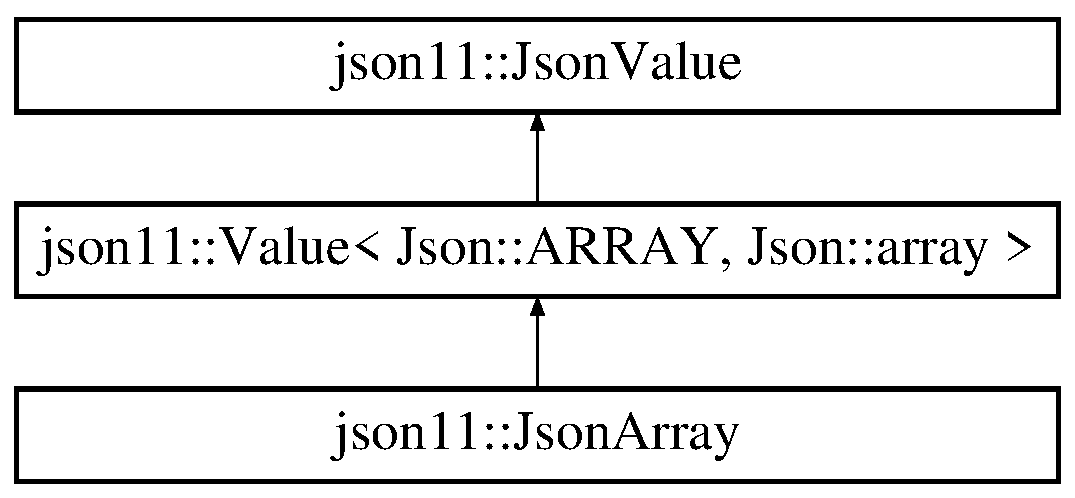
\includegraphics[height=3.000000cm]{classjson11_1_1_json_array}
\end{center}
\end{figure}
\subsection*{Public Member Functions}
\begin{DoxyCompactItemize}
\item 
\mbox{\Hypertarget{classjson11_1_1_json_array_a305a9591c44b22ffc91a371b8248d5a4}\label{classjson11_1_1_json_array_a305a9591c44b22ffc91a371b8248d5a4}} 
{\bfseries Json\+Array} (const Json\+::array \&value)
\item 
\mbox{\Hypertarget{classjson11_1_1_json_array_ae360edbd727b3126f7174c86a24003e1}\label{classjson11_1_1_json_array_ae360edbd727b3126f7174c86a24003e1}} 
{\bfseries Json\+Array} (Json\+::array \&\&value)
\end{DoxyCompactItemize}
\subsection*{Additional Inherited Members}


The documentation for this class was generated from the following file\+:\begin{DoxyCompactItemize}
\item 
/\+Users/h\+Gen/\+Desktop/qt/glwarp-\/configuration-\/tool/src/lib/json11.\+cpp\end{DoxyCompactItemize}

\hypertarget{classjson11_1_1_json_boolean}{}\section{json11\+:\+:Json\+Boolean Class Reference}
\label{classjson11_1_1_json_boolean}\index{json11\+::\+Json\+Boolean@{json11\+::\+Json\+Boolean}}
Inheritance diagram for json11\+:\+:Json\+Boolean\+:\begin{figure}[H]
\begin{center}
\leavevmode
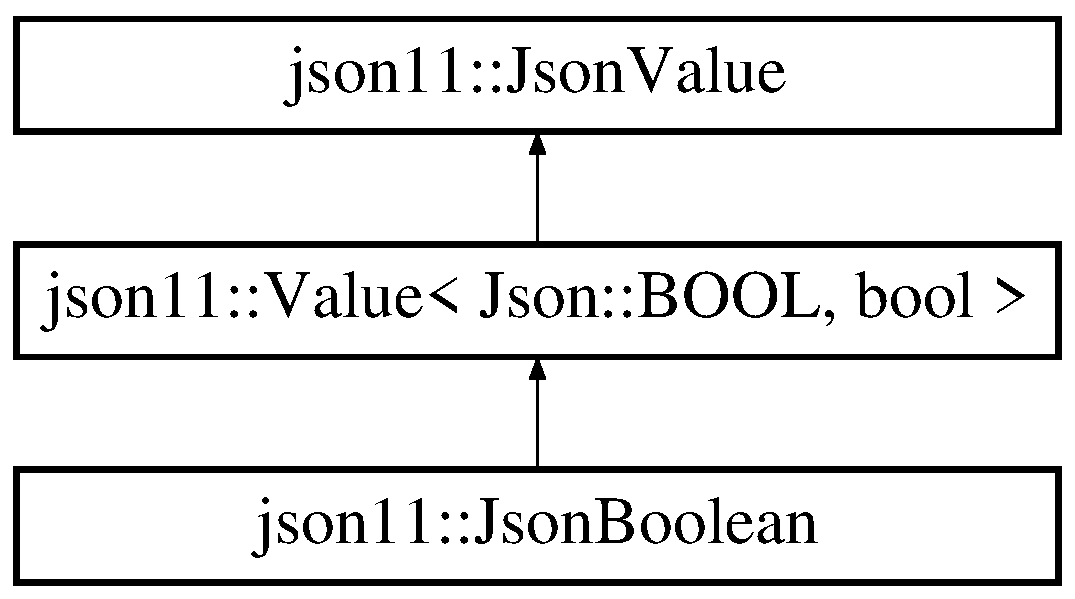
\includegraphics[height=3.000000cm]{classjson11_1_1_json_boolean}
\end{center}
\end{figure}
\subsection*{Public Member Functions}
\begin{DoxyCompactItemize}
\item 
\mbox{\Hypertarget{classjson11_1_1_json_boolean_a23d0577d5fd615eafad0d74f0b632ba4}\label{classjson11_1_1_json_boolean_a23d0577d5fd615eafad0d74f0b632ba4}} 
{\bfseries Json\+Boolean} (bool value)
\end{DoxyCompactItemize}
\subsection*{Additional Inherited Members}


The documentation for this class was generated from the following file\+:\begin{DoxyCompactItemize}
\item 
/\+Users/h\+Gen/\+Desktop/qt/glwarp-\/configuration-\/tool/src/lib/json11.\+cpp\end{DoxyCompactItemize}

\hypertarget{classjson11_1_1_json_double}{}\section{json11\+:\+:Json\+Double Class Reference}
\label{classjson11_1_1_json_double}\index{json11\+::\+Json\+Double@{json11\+::\+Json\+Double}}
Inheritance diagram for json11\+:\+:Json\+Double\+:\begin{figure}[H]
\begin{center}
\leavevmode
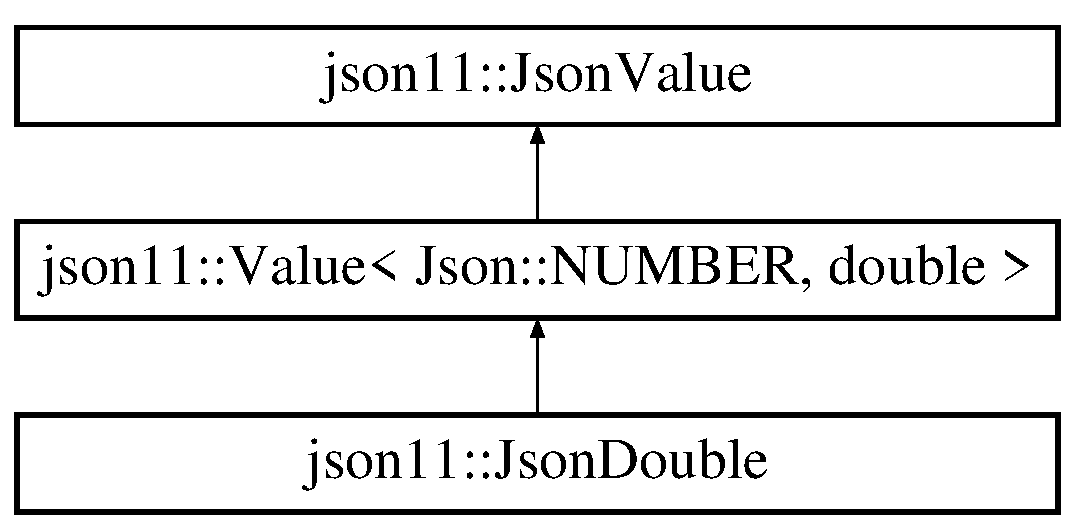
\includegraphics[height=3.000000cm]{classjson11_1_1_json_double}
\end{center}
\end{figure}
\subsection*{Public Member Functions}
\begin{DoxyCompactItemize}
\item 
\mbox{\Hypertarget{classjson11_1_1_json_double_a58b161847d227681e6d6e3f2a714af07}\label{classjson11_1_1_json_double_a58b161847d227681e6d6e3f2a714af07}} 
{\bfseries Json\+Double} (double value)
\end{DoxyCompactItemize}
\subsection*{Additional Inherited Members}


The documentation for this class was generated from the following file\+:\begin{DoxyCompactItemize}
\item 
/\+Users/h\+Gen/\+Desktop/qt/glwarp-\/configuration-\/tool/src/lib/json11.\+cpp\end{DoxyCompactItemize}

\hypertarget{classjson11_1_1_json_int}{}\section{json11\+:\+:Json\+Int Class Reference}
\label{classjson11_1_1_json_int}\index{json11\+::\+Json\+Int@{json11\+::\+Json\+Int}}
Inheritance diagram for json11\+:\+:Json\+Int\+:\begin{figure}[H]
\begin{center}
\leavevmode
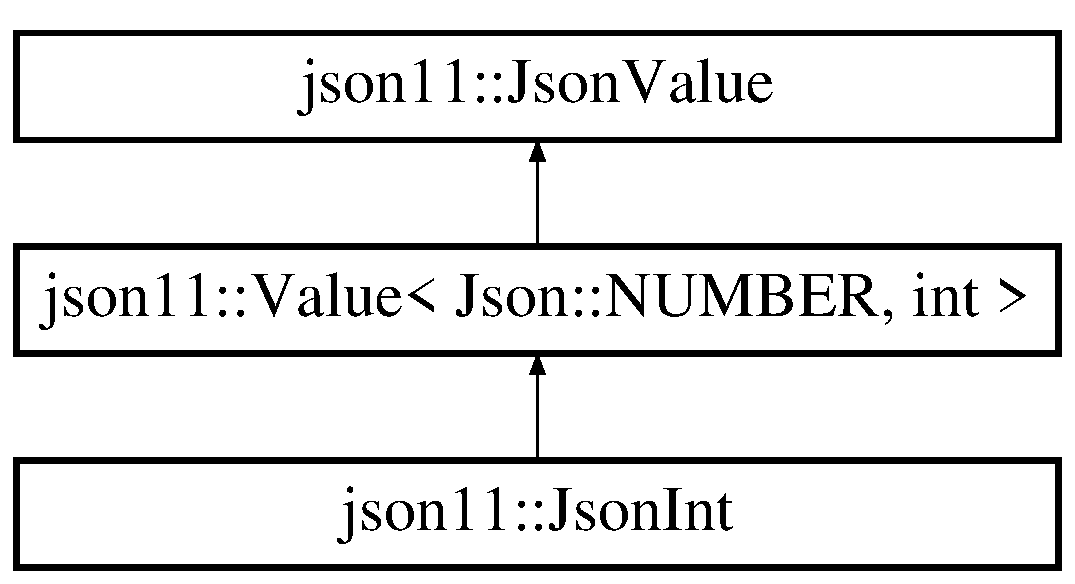
\includegraphics[height=3.000000cm]{classjson11_1_1_json_int}
\end{center}
\end{figure}
\subsection*{Public Member Functions}
\begin{DoxyCompactItemize}
\item 
\mbox{\Hypertarget{classjson11_1_1_json_int_a8e1607a772d00863178dfd3b7d4e9e6e}\label{classjson11_1_1_json_int_a8e1607a772d00863178dfd3b7d4e9e6e}} 
{\bfseries Json\+Int} (int value)
\end{DoxyCompactItemize}
\subsection*{Additional Inherited Members}


The documentation for this class was generated from the following file\+:\begin{DoxyCompactItemize}
\item 
/\+Users/h\+Gen/\+Desktop/qt/glwarp-\/configuration-\/tool/src/lib/json11.\+cpp\end{DoxyCompactItemize}

\hypertarget{classjson11_1_1_json_null}{}\section{json11\+:\+:Json\+Null Class Reference}
\label{classjson11_1_1_json_null}\index{json11\+::\+Json\+Null@{json11\+::\+Json\+Null}}
Inheritance diagram for json11\+:\+:Json\+Null\+:\begin{figure}[H]
\begin{center}
\leavevmode
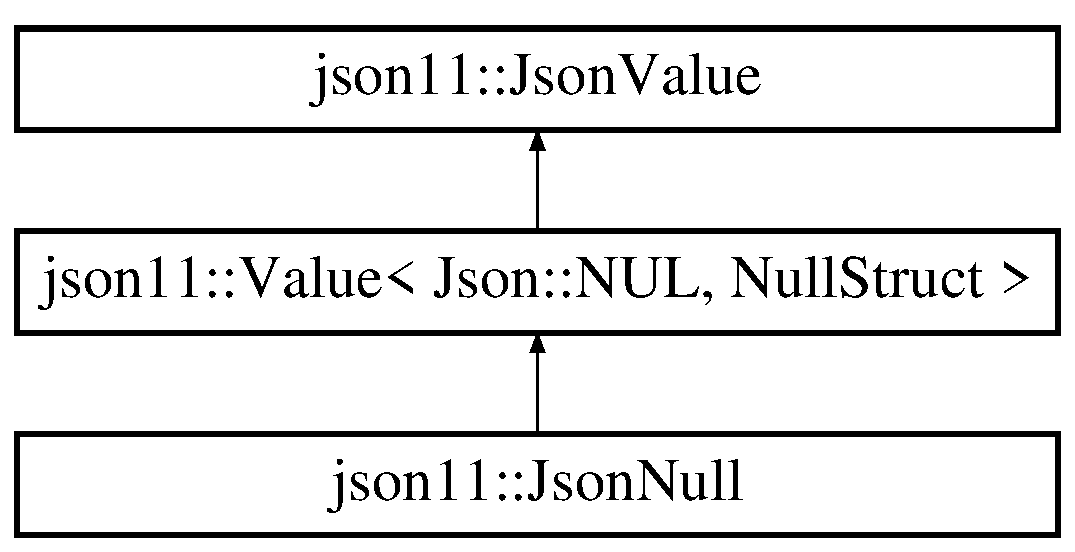
\includegraphics[height=3.000000cm]{classjson11_1_1_json_null}
\end{center}
\end{figure}
\subsection*{Additional Inherited Members}


The documentation for this class was generated from the following file\+:\begin{DoxyCompactItemize}
\item 
/\+Users/h\+Gen/\+Desktop/qt/glwarp-\/configuration-\/tool/src/lib/json11.\+cpp\end{DoxyCompactItemize}

\hypertarget{classjson11_1_1_json_object}{}\section{json11\+:\+:Json\+Object Class Reference}
\label{classjson11_1_1_json_object}\index{json11\+::\+Json\+Object@{json11\+::\+Json\+Object}}
Inheritance diagram for json11\+:\+:Json\+Object\+:\begin{figure}[H]
\begin{center}
\leavevmode
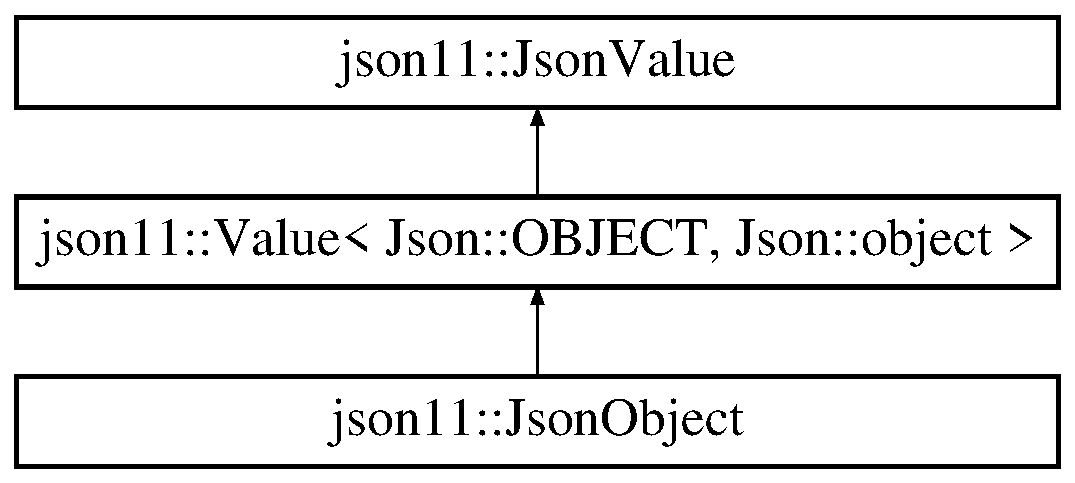
\includegraphics[height=3.000000cm]{classjson11_1_1_json_object}
\end{center}
\end{figure}
\subsection*{Public Member Functions}
\begin{DoxyCompactItemize}
\item 
\mbox{\Hypertarget{classjson11_1_1_json_object_a078da3ed9d93649f3c3a717d347ac94a}\label{classjson11_1_1_json_object_a078da3ed9d93649f3c3a717d347ac94a}} 
{\bfseries Json\+Object} (const Json\+::object \&value)
\item 
\mbox{\Hypertarget{classjson11_1_1_json_object_a22c01f3ec1b8e78bc341375c755184f2}\label{classjson11_1_1_json_object_a22c01f3ec1b8e78bc341375c755184f2}} 
{\bfseries Json\+Object} (Json\+::object \&\&value)
\end{DoxyCompactItemize}
\subsection*{Additional Inherited Members}


The documentation for this class was generated from the following file\+:\begin{DoxyCompactItemize}
\item 
/\+Users/h\+Gen/\+Desktop/qt/glwarp-\/configuration-\/tool/src/lib/json11.\+cpp\end{DoxyCompactItemize}

\hypertarget{classjson11_1_1_json_string}{}\section{json11\+:\+:Json\+String Class Reference}
\label{classjson11_1_1_json_string}\index{json11\+::\+Json\+String@{json11\+::\+Json\+String}}
Inheritance diagram for json11\+:\+:Json\+String\+:\begin{figure}[H]
\begin{center}
\leavevmode
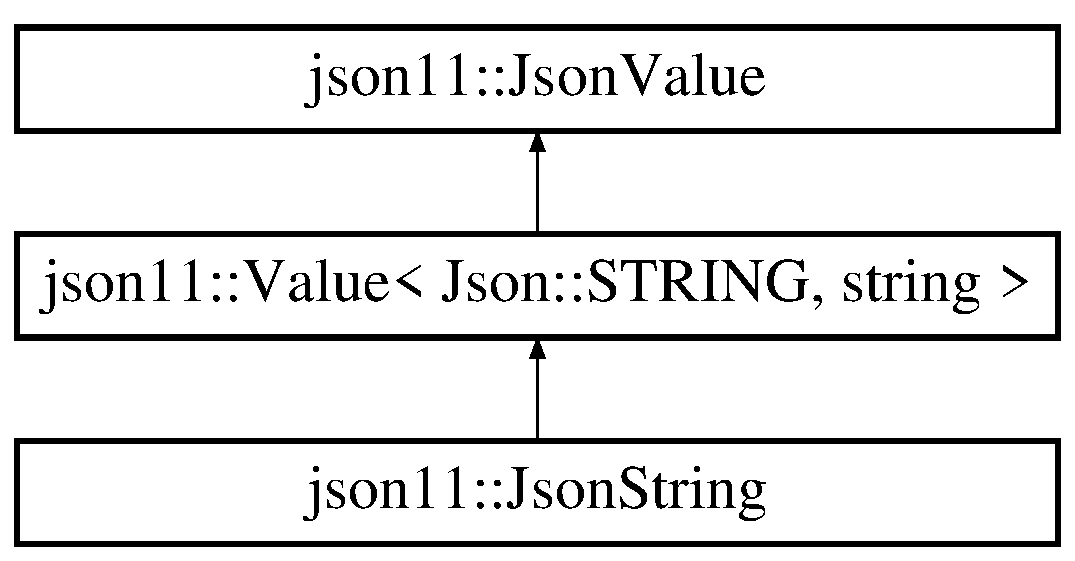
\includegraphics[height=3.000000cm]{classjson11_1_1_json_string}
\end{center}
\end{figure}
\subsection*{Public Member Functions}
\begin{DoxyCompactItemize}
\item 
\mbox{\Hypertarget{classjson11_1_1_json_string_a367de25bb5eae5a41abea569646eca12}\label{classjson11_1_1_json_string_a367de25bb5eae5a41abea569646eca12}} 
{\bfseries Json\+String} (const string \&value)
\item 
\mbox{\Hypertarget{classjson11_1_1_json_string_a4c2722034ef127dae2573025e6b606b6}\label{classjson11_1_1_json_string_a4c2722034ef127dae2573025e6b606b6}} 
{\bfseries Json\+String} (string \&\&value)
\end{DoxyCompactItemize}
\subsection*{Additional Inherited Members}


The documentation for this class was generated from the following file\+:\begin{DoxyCompactItemize}
\item 
/\+Users/h\+Gen/\+Desktop/qt/glwarp-\/configuration-\/tool/src/lib/json11.\+cpp\end{DoxyCompactItemize}

\hypertarget{classjson11_1_1_json_value}{}\section{json11\+:\+:Json\+Value Class Reference}
\label{classjson11_1_1_json_value}\index{json11\+::\+Json\+Value@{json11\+::\+Json\+Value}}
Inheritance diagram for json11\+:\+:Json\+Value\+:\begin{figure}[H]
\begin{center}
\leavevmode
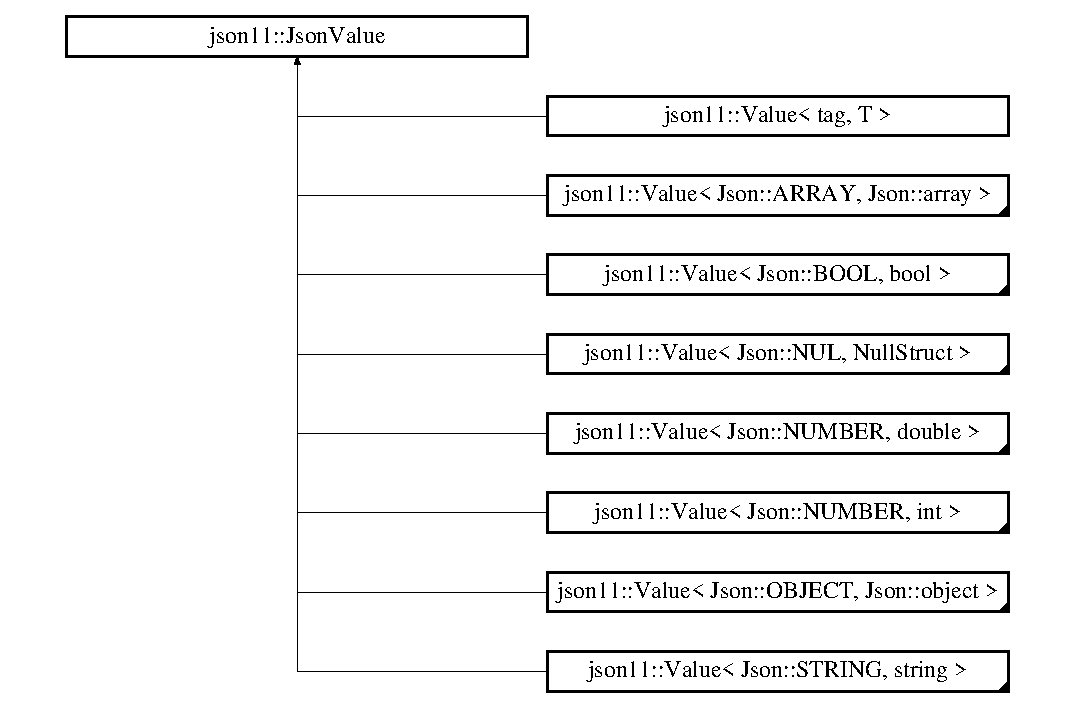
\includegraphics[height=9.000000cm]{classjson11_1_1_json_value}
\end{center}
\end{figure}
\subsection*{Protected Member Functions}
\begin{DoxyCompactItemize}
\item 
\mbox{\Hypertarget{classjson11_1_1_json_value_abad3377adfead681fdf42c5c6aec6b2a}\label{classjson11_1_1_json_value_abad3377adfead681fdf42c5c6aec6b2a}} 
virtual Json\+::\+Type {\bfseries type} () const =0
\item 
\mbox{\Hypertarget{classjson11_1_1_json_value_a2730125126e440ecb6ef5de9f2ce8ddf}\label{classjson11_1_1_json_value_a2730125126e440ecb6ef5de9f2ce8ddf}} 
virtual bool {\bfseries equals} (const \mbox{\hyperlink{classjson11_1_1_json_value}{Json\+Value}} $\ast$other) const =0
\item 
\mbox{\Hypertarget{classjson11_1_1_json_value_a028ef0c49d746853c69c36cd784ce862}\label{classjson11_1_1_json_value_a028ef0c49d746853c69c36cd784ce862}} 
virtual bool {\bfseries less} (const \mbox{\hyperlink{classjson11_1_1_json_value}{Json\+Value}} $\ast$other) const =0
\item 
\mbox{\Hypertarget{classjson11_1_1_json_value_a7b091df08f99eb9e8c01554b2c058c86}\label{classjson11_1_1_json_value_a7b091df08f99eb9e8c01554b2c058c86}} 
virtual void {\bfseries dump} (std\+::string \&out) const =0
\item 
\mbox{\Hypertarget{classjson11_1_1_json_value_add546ac727d19c92888028745bd71713}\label{classjson11_1_1_json_value_add546ac727d19c92888028745bd71713}} 
virtual double {\bfseries number\+\_\+value} () const
\item 
\mbox{\Hypertarget{classjson11_1_1_json_value_a35bcf1583c7d9e14ebc0aba745670dbf}\label{classjson11_1_1_json_value_a35bcf1583c7d9e14ebc0aba745670dbf}} 
virtual int {\bfseries int\+\_\+value} () const
\item 
\mbox{\Hypertarget{classjson11_1_1_json_value_a0f239dbb429278cc00573e4bcadce866}\label{classjson11_1_1_json_value_a0f239dbb429278cc00573e4bcadce866}} 
virtual bool {\bfseries bool\+\_\+value} () const
\item 
\mbox{\Hypertarget{classjson11_1_1_json_value_a504b77271f3aab4ff4a7e61653b9c264}\label{classjson11_1_1_json_value_a504b77271f3aab4ff4a7e61653b9c264}} 
virtual const std\+::string \& {\bfseries string\+\_\+value} () const
\item 
\mbox{\Hypertarget{classjson11_1_1_json_value_a66c1fec1624e25ede589dc541f2b5913}\label{classjson11_1_1_json_value_a66c1fec1624e25ede589dc541f2b5913}} 
virtual const Json\+::array \& {\bfseries array\+\_\+items} () const
\item 
\mbox{\Hypertarget{classjson11_1_1_json_value_a8e87087afb53fceb8350f7bc1e28c18f}\label{classjson11_1_1_json_value_a8e87087afb53fceb8350f7bc1e28c18f}} 
virtual const \mbox{\hyperlink{classjson11_1_1_json}{Json}} \& {\bfseries operator\mbox{[}$\,$\mbox{]}} (size\+\_\+t i) const
\item 
\mbox{\Hypertarget{classjson11_1_1_json_value_a42b4e842ac0697004e7ba76646a6f9be}\label{classjson11_1_1_json_value_a42b4e842ac0697004e7ba76646a6f9be}} 
virtual const Json\+::object \& {\bfseries object\+\_\+items} () const
\item 
\mbox{\Hypertarget{classjson11_1_1_json_value_abb082ed22afec495df30552bb4c67248}\label{classjson11_1_1_json_value_abb082ed22afec495df30552bb4c67248}} 
virtual const \mbox{\hyperlink{classjson11_1_1_json}{Json}} \& {\bfseries operator\mbox{[}$\,$\mbox{]}} (const std\+::string \&key) const
\end{DoxyCompactItemize}
\subsection*{Friends}
\begin{DoxyCompactItemize}
\item 
\mbox{\Hypertarget{classjson11_1_1_json_value_a7dd8a79e9210a2a230d000eee63c6e8a}\label{classjson11_1_1_json_value_a7dd8a79e9210a2a230d000eee63c6e8a}} 
class {\bfseries Json}
\item 
\mbox{\Hypertarget{classjson11_1_1_json_value_a4079b619596181593da9d6fde75ee2f3}\label{classjson11_1_1_json_value_a4079b619596181593da9d6fde75ee2f3}} 
class {\bfseries Json\+Int}
\item 
\mbox{\Hypertarget{classjson11_1_1_json_value_a0bdd38d55ffef87604233cb81a887f47}\label{classjson11_1_1_json_value_a0bdd38d55ffef87604233cb81a887f47}} 
class {\bfseries Json\+Double}
\end{DoxyCompactItemize}


The documentation for this class was generated from the following files\+:\begin{DoxyCompactItemize}
\item 
/\+Users/h\+Gen/\+Desktop/qt/glwarp-\/configuration-\/tool/src/lib/json11.\+hpp\item 
/\+Users/h\+Gen/\+Desktop/qt/glwarp-\/configuration-\/tool/src/lib/json11.\+cpp\end{DoxyCompactItemize}

\hypertarget{class_main_widget}{}\section{Main\+Widget Class Reference}
\label{class_main_widget}\index{Main\+Widget@{Main\+Widget}}
Inheritance diagram for Main\+Widget\+:\begin{figure}[H]
\begin{center}
\leavevmode
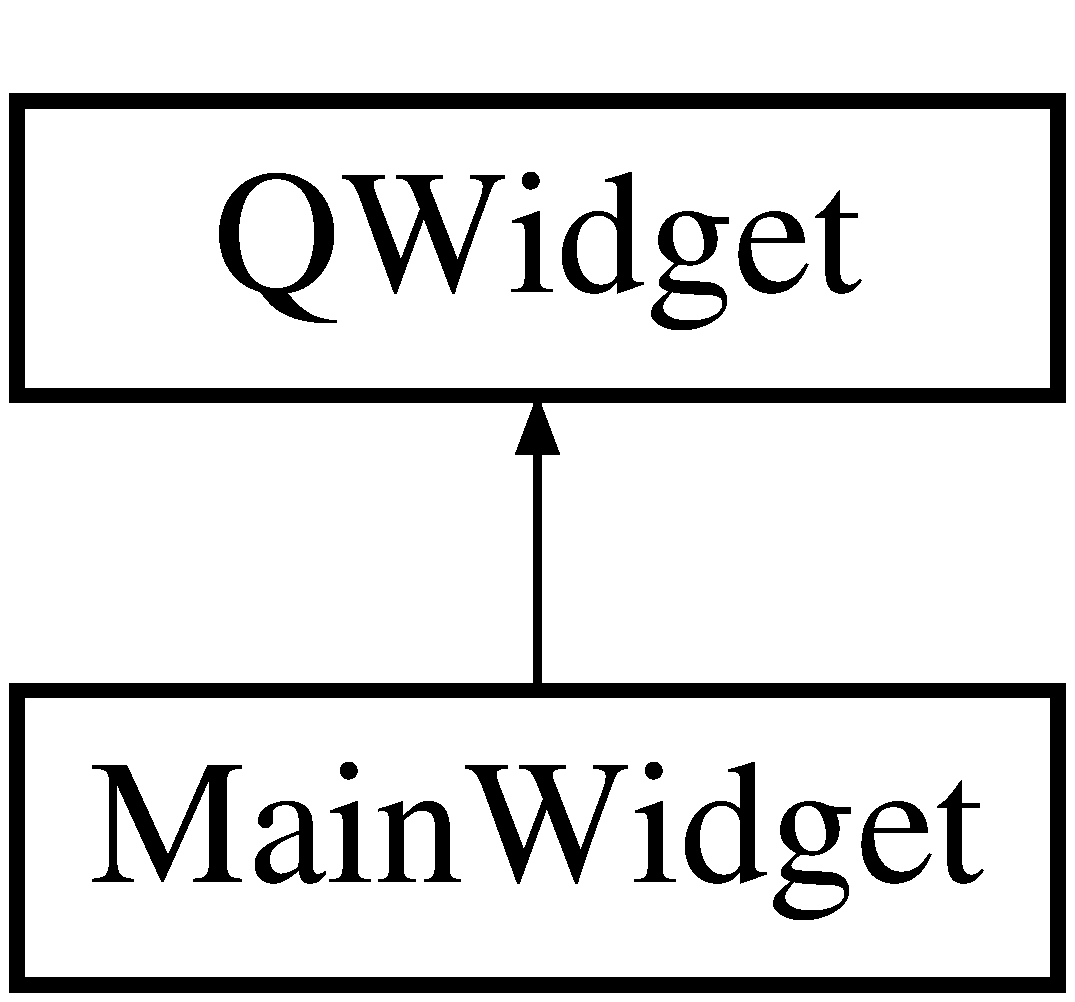
\includegraphics[height=2.000000cm]{class_main_widget}
\end{center}
\end{figure}
\subsection*{Public Slots}
\begin{DoxyCompactItemize}
\item 
\mbox{\Hypertarget{class_main_widget_af956e8da220cd6ca378cfc0eff118fda}\label{class_main_widget_af956e8da220cd6ca378cfc0eff118fda}} 
void \mbox{\hyperlink{class_main_widget_af956e8da220cd6ca378cfc0eff118fda}{on\+Open\+Transformation\+View}} ()
\begin{DoxyCompactList}\small\item\em Opens the transformation view in a separate window to view a simulation of the current set parameters. \end{DoxyCompactList}\item 
\mbox{\Hypertarget{class_main_widget_aaef2b6704ce08fc8b2e5ed875fb6723a}\label{class_main_widget_aaef2b6704ce08fc8b2e5ed875fb6723a}} 
void \mbox{\hyperlink{class_main_widget_aaef2b6704ce08fc8b2e5ed875fb6723a}{on\+Load\+Custom\+Config}} ()
\begin{DoxyCompactList}\small\item\em This funciton either loads the default simluation and UI values or opens a file dialog from which a custom configuration file can be specified. \end{DoxyCompactList}\item 
\mbox{\Hypertarget{class_main_widget_ac0de890595886748baeb468f5b234f0f}\label{class_main_widget_ac0de890595886748baeb468f5b234f0f}} 
void \mbox{\hyperlink{class_main_widget_ac0de890595886748baeb468f5b234f0f}{on\+Save\+Model\+Config}} ()
\begin{DoxyCompactList}\small\item\em on\+Save\+Model\+Config \end{DoxyCompactList}\end{DoxyCompactItemize}
\subsection*{Public Member Functions}
\begin{DoxyCompactItemize}
\item 
\mbox{\hyperlink{class_main_widget_a279f84c512f46833e33991b0f363492f}{Main\+Widget}} (\mbox{\hyperlink{class_main_window}{Main\+Window}} $\ast$mw)
\begin{DoxyCompactList}\small\item\em \mbox{\hyperlink{class_main_widget}{Main\+Widget}}. \end{DoxyCompactList}\item 
\mbox{\Hypertarget{class_main_widget_a001d36b58ef82d9866e2ab3ea082f0d4}\label{class_main_widget_a001d36b58ef82d9866e2ab3ea082f0d4}} 
Q\+Menu $\ast$ {\bfseries get\+Menu} ()
\end{DoxyCompactItemize}


\subsection{Constructor \& Destructor Documentation}
\mbox{\Hypertarget{class_main_widget_a279f84c512f46833e33991b0f363492f}\label{class_main_widget_a279f84c512f46833e33991b0f363492f}} 
\index{Main\+Widget@{Main\+Widget}!Main\+Widget@{Main\+Widget}}
\index{Main\+Widget@{Main\+Widget}!Main\+Widget@{Main\+Widget}}
\subsubsection{\texorpdfstring{Main\+Widget()}{MainWidget()}}
{\footnotesize\ttfamily Main\+Widget\+::\+Main\+Widget (\begin{DoxyParamCaption}\item[{\mbox{\hyperlink{class_main_window}{Main\+Window}} $\ast$}]{mw }\end{DoxyParamCaption})}



\mbox{\hyperlink{class_main_widget}{Main\+Widget}}. 


\begin{DoxyParams}{Parameters}
{\em mw} & \\
\hline
\end{DoxyParams}


The documentation for this class was generated from the following files\+:\begin{DoxyCompactItemize}
\item 
/\+Users/h\+Gen/\+Desktop/qt/glwarp-\/configuration-\/tool/src/ui/mainwidget.\+h\item 
/\+Users/h\+Gen/\+Desktop/qt/glwarp-\/configuration-\/tool/src/ui/mainwidget.\+cpp\end{DoxyCompactItemize}

\hypertarget{class_main_window}{}\section{Main\+Window Class Reference}
\label{class_main_window}\index{Main\+Window@{Main\+Window}}
Inheritance diagram for Main\+Window\+:\begin{figure}[H]
\begin{center}
\leavevmode
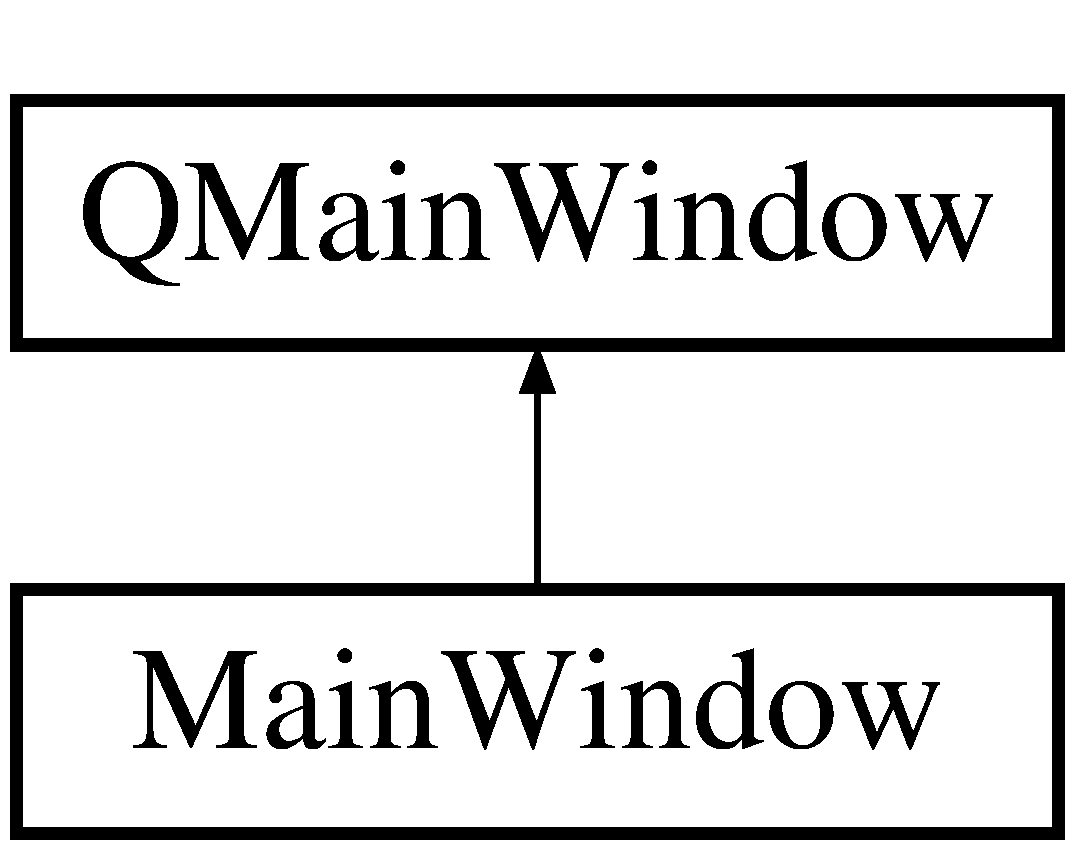
\includegraphics[height=2.000000cm]{class_main_window}
\end{center}
\end{figure}
\subsection*{Public Member Functions}
\begin{DoxyCompactItemize}
\item 
\mbox{\Hypertarget{class_main_window_a8b244be8b7b7db1b08de2a2acb9409db}\label{class_main_window_a8b244be8b7b7db1b08de2a2acb9409db}} 
{\bfseries Main\+Window} (Q\+Widget $\ast$parent=0)
\end{DoxyCompactItemize}


The documentation for this class was generated from the following files\+:\begin{DoxyCompactItemize}
\item 
/\+Users/h\+Gen/\+Desktop/qt/glwarp-\/configuration-\/tool/src/ui/mainwindow.\+h\item 
/\+Users/h\+Gen/\+Desktop/qt/glwarp-\/configuration-\/tool/src/ui/mainwindow.\+cpp\end{DoxyCompactItemize}

\hypertarget{struct_model_config}{}\section{Model\+Config Struct Reference}
\label{struct_model_config}\index{Model\+Config@{Model\+Config}}
\subsection*{Static Public Member Functions}
\begin{DoxyCompactItemize}
\item 
\mbox{\Hypertarget{struct_model_config_a91b93e14eb8340c9ddc69803086fdaa9}\label{struct_model_config_a91b93e14eb8340c9ddc69803086fdaa9}} 
static \mbox{\hyperlink{struct_model_config}{Model\+Config}} {\bfseries from\+Json} (const Q\+Json\+Object \&object)
\end{DoxyCompactItemize}
\subsection*{Public Attributes}
\begin{DoxyCompactItemize}
\item 
\mbox{\Hypertarget{struct_model_config_a3ccee2fc963e2e10d120d52c67b3078e}\label{struct_model_config_a3ccee2fc963e2e10d120d52c67b3078e}} 
\mbox{\hyperlink{struct_dome_projector_config}{Dome\+Projector\+Config}} {\bfseries dome\+\_\+projector}
\item 
\mbox{\Hypertarget{struct_model_config_a48f3bfe8ddf6e9bdb753b298e90800a7}\label{struct_model_config_a48f3bfe8ddf6e9bdb753b298e90800a7}} 
\mbox{\hyperlink{struct_sphere_config}{Sphere\+Config}} {\bfseries dome}
\item 
\mbox{\Hypertarget{struct_model_config_a5b1cd485659bfe6009bbdba15e362e7c}\label{struct_model_config_a5b1cd485659bfe6009bbdba15e362e7c}} 
\mbox{\hyperlink{struct_sphere_config}{Sphere\+Config}} {\bfseries mirror}
\end{DoxyCompactItemize}


The documentation for this struct was generated from the following files\+:\begin{DoxyCompactItemize}
\item 
/\+Users/h\+Gen/\+Desktop/qt/glwarp-\/configuration-\/tool/src/config.\+h\item 
/\+Users/h\+Gen/\+Desktop/qt/glwarp-\/configuration-\/tool/src/config.\+cpp\end{DoxyCompactItemize}

\hypertarget{structjson11_1_1_null_struct}{}\section{json11\+:\+:Null\+Struct Struct Reference}
\label{structjson11_1_1_null_struct}\index{json11\+::\+Null\+Struct@{json11\+::\+Null\+Struct}}
\subsection*{Public Member Functions}
\begin{DoxyCompactItemize}
\item 
\mbox{\Hypertarget{structjson11_1_1_null_struct_a29752d42bbc3bdf8933ad57590a34a2d}\label{structjson11_1_1_null_struct_a29752d42bbc3bdf8933ad57590a34a2d}} 
bool {\bfseries operator==} (\mbox{\hyperlink{structjson11_1_1_null_struct}{Null\+Struct}}) const
\item 
\mbox{\Hypertarget{structjson11_1_1_null_struct_afe7c5e06a64fc0d83a6ff2393b71609d}\label{structjson11_1_1_null_struct_afe7c5e06a64fc0d83a6ff2393b71609d}} 
bool {\bfseries operator$<$} (\mbox{\hyperlink{structjson11_1_1_null_struct}{Null\+Struct}}) const
\end{DoxyCompactItemize}


The documentation for this struct was generated from the following file\+:\begin{DoxyCompactItemize}
\item 
/\+Users/h\+Gen/\+Desktop/qt/glwarp-\/configuration-\/tool/src/lib/json11.\+cpp\end{DoxyCompactItemize}

\hypertarget{class_path}{}\section{Path Class Reference}
\label{class_path}\index{Path@{Path}}


The \mbox{\hyperlink{class_path}{Path}} class holds a vector and acts as a more fail save way of handling paths.  




{\ttfamily \#include $<$path.\+hpp$>$}

\subsection*{Public Member Functions}
\begin{DoxyCompactItemize}
\item 
\mbox{\hyperlink{class_path_af26cfab021ddf49af73da3b2beca85ac}{Path}} ()
\item 
\mbox{\hyperlink{class_path_ae560f045f52d39eacdac15ec28b0b8b8}{Path}} (std\+::string const \&path)
\item 
\mbox{\hyperlink{class_path_ab8cc1ce5a7c3f79bb5e730fd847c846e}{Path}} (std\+::vector$<$ std\+::string $>$ const \&path)
\item 
void \mbox{\hyperlink{class_path_af270e6e39de7389980e4c6d0cf9fdd37}{push\+\_\+s}} (std\+::string const \&path)
\item 
void \mbox{\hyperlink{class_path_a32a30af9ac4989b875079b01ff9d2825}{push\+\_\+m}} (std\+::vector$<$ std\+::string $>$ const \&path)
\item 
void \mbox{\hyperlink{class_path_a0f02b5b2384900e3fe1c3efadea6c0ca}{pop}} ()
\item 
std\+::string const  \& \mbox{\hyperlink{class_path_a7c1a4772ea53d546d9cd2dad199fd633}{str}} () const
\end{DoxyCompactItemize}


\subsection{Detailed Description}
The \mbox{\hyperlink{class_path}{Path}} class holds a vector and acts as a more fail save way of handling paths. 

This was introduced way before a Qt UI had been planned. Using Q\+Dir instead might make sense. 

\subsection{Constructor \& Destructor Documentation}
\mbox{\Hypertarget{class_path_af26cfab021ddf49af73da3b2beca85ac}\label{class_path_af26cfab021ddf49af73da3b2beca85ac}} 
\index{Path@{Path}!Path@{Path}}
\index{Path@{Path}!Path@{Path}}
\subsubsection{\texorpdfstring{Path()}{Path()}\hspace{0.1cm}{\footnotesize\ttfamily [1/3]}}
{\footnotesize\ttfamily Path\+::\+Path (\begin{DoxyParamCaption}{ }\end{DoxyParamCaption})}

Empty c\textquotesingle{}tor \mbox{\Hypertarget{class_path_ae560f045f52d39eacdac15ec28b0b8b8}\label{class_path_ae560f045f52d39eacdac15ec28b0b8b8}} 
\index{Path@{Path}!Path@{Path}}
\index{Path@{Path}!Path@{Path}}
\subsubsection{\texorpdfstring{Path()}{Path()}\hspace{0.1cm}{\footnotesize\ttfamily [2/3]}}
{\footnotesize\ttfamily Path\+::\+Path (\begin{DoxyParamCaption}\item[{std\+::string const \&}]{path }\end{DoxyParamCaption})}

Constructs a \mbox{\hyperlink{class_path}{Path}} object containing an initial directory. 
\begin{DoxyParams}{Parameters}
{\em path} & \\
\hline
\end{DoxyParams}
\mbox{\Hypertarget{class_path_ab8cc1ce5a7c3f79bb5e730fd847c846e}\label{class_path_ab8cc1ce5a7c3f79bb5e730fd847c846e}} 
\index{Path@{Path}!Path@{Path}}
\index{Path@{Path}!Path@{Path}}
\subsubsection{\texorpdfstring{Path()}{Path()}\hspace{0.1cm}{\footnotesize\ttfamily [3/3]}}
{\footnotesize\ttfamily Path\+::\+Path (\begin{DoxyParamCaption}\item[{std\+::vector$<$ std\+::string $>$ const \&}]{path }\end{DoxyParamCaption})}

Constructs a \mbox{\hyperlink{class_path}{Path}} object by passing std\+::vector of std\+::strings. 
\begin{DoxyParams}{Parameters}
{\em path} & \\
\hline
\end{DoxyParams}


\subsection{Member Function Documentation}
\mbox{\Hypertarget{class_path_a0f02b5b2384900e3fe1c3efadea6c0ca}\label{class_path_a0f02b5b2384900e3fe1c3efadea6c0ca}} 
\index{Path@{Path}!pop@{pop}}
\index{pop@{pop}!Path@{Path}}
\subsubsection{\texorpdfstring{pop()}{pop()}}
{\footnotesize\ttfamily void Path\+::pop (\begin{DoxyParamCaption}{ }\end{DoxyParamCaption})}

Removes the last paths element. \mbox{\Hypertarget{class_path_a32a30af9ac4989b875079b01ff9d2825}\label{class_path_a32a30af9ac4989b875079b01ff9d2825}} 
\index{Path@{Path}!push\+\_\+m@{push\+\_\+m}}
\index{push\+\_\+m@{push\+\_\+m}!Path@{Path}}
\subsubsection{\texorpdfstring{push\+\_\+m()}{push\_m()}}
{\footnotesize\ttfamily void Path\+::push\+\_\+m (\begin{DoxyParamCaption}\item[{std\+::vector$<$ std\+::string $>$ const \&}]{path }\end{DoxyParamCaption})}

Pushes multiple elements to the end of the string. from std\+::vector$<$std\+::string$>$$>$ 
\begin{DoxyParams}{Parameters}
{\em path} & \\
\hline
\end{DoxyParams}
\mbox{\Hypertarget{class_path_af270e6e39de7389980e4c6d0cf9fdd37}\label{class_path_af270e6e39de7389980e4c6d0cf9fdd37}} 
\index{Path@{Path}!push\+\_\+s@{push\+\_\+s}}
\index{push\+\_\+s@{push\+\_\+s}!Path@{Path}}
\subsubsection{\texorpdfstring{push\+\_\+s()}{push\_s()}}
{\footnotesize\ttfamily void Path\+::push\+\_\+s (\begin{DoxyParamCaption}\item[{std\+::string const \&}]{path }\end{DoxyParamCaption})}

Pushes a single object to the end of the string. 
\begin{DoxyParams}{Parameters}
{\em path} & \\
\hline
\end{DoxyParams}
\mbox{\Hypertarget{class_path_a7c1a4772ea53d546d9cd2dad199fd633}\label{class_path_a7c1a4772ea53d546d9cd2dad199fd633}} 
\index{Path@{Path}!str@{str}}
\index{str@{str}!Path@{Path}}
\subsubsection{\texorpdfstring{str()}{str()}}
{\footnotesize\ttfamily std\+::string const  \& Path\+::str (\begin{DoxyParamCaption}{ }\end{DoxyParamCaption}) const}

Returns std\+::string from path. \begin{DoxyReturn}{Returns}
std\+::string const\& 
\end{DoxyReturn}


The documentation for this class was generated from the following files\+:\begin{DoxyCompactItemize}
\item 
/\+Users/h\+Gen/\+Desktop/qt/glwarp-\/configuration-\/tool/src/model/path.\+hpp\item 
/\+Users/h\+Gen/\+Desktop/qt/glwarp-\/configuration-\/tool/src/model/path.\+cpp\end{DoxyCompactItemize}

\hypertarget{class_projector_frustum}{}\section{Projector\+Frustum Class Reference}
\label{class_projector_frustum}\index{Projector\+Frustum@{Projector\+Frustum}}


The \mbox{\hyperlink{class_projector_frustum}{Projector\+Frustum}} class describes a light projector frustum.  




{\ttfamily \#include $<$projector\+\_\+frustum.\+hpp$>$}

\subsection*{Public Types}
\begin{DoxyCompactItemize}
\item 
\mbox{\Hypertarget{class_projector_frustum_ada11c8a7dc78a009ac6a7fd8667c264b}\label{class_projector_frustum_ada11c8a7dc78a009ac6a7fd8667c264b}} 
enum {\bfseries Clipping\+Plane} \{ {\bfseries N\+E\+AR}, 
{\bfseries F\+AR}
 \}
\item 
\mbox{\Hypertarget{class_projector_frustum_a3ed65cdb2799b84b6d8341ee77e69c74}\label{class_projector_frustum_a3ed65cdb2799b84b6d8341ee77e69c74}} 
enum {\bfseries Corner} \{ {\bfseries TL}, 
{\bfseries TR}, 
{\bfseries BL}, 
{\bfseries BR}
 \}
\end{DoxyCompactItemize}
\subsection*{Public Member Functions}
\begin{DoxyCompactItemize}
\item 
\mbox{\Hypertarget{class_projector_frustum_aaddf578aae0115cd79ba29dc878ae545}\label{class_projector_frustum_aaddf578aae0115cd79ba29dc878ae545}} 
\mbox{\hyperlink{class_projector_frustum_aaddf578aae0115cd79ba29dc878ae545}{Projector\+Frustum}} ()
\begin{DoxyCompactList}\small\item\em \mbox{\hyperlink{class_projector_frustum}{Projector\+Frustum}}. \end{DoxyCompactList}\item 
\mbox{\hyperlink{class_projector_frustum_aac915f2a3a87868d11f0bb66a18342db}{Projector\+Frustum}} (float \+\_\+aspect\+\_\+ratio, float \+\_\+fov, float \+\_\+near, float \+\_\+far)
\begin{DoxyCompactList}\small\item\em Creates a new frustum with the given values. \end{DoxyCompactList}\item 
void \mbox{\hyperlink{class_projector_frustum_a1c5c97e807392f1e828c050ef17bcc92}{translate}} (Q\+Vector3D const \&position)
\begin{DoxyCompactList}\small\item\em Translate to current position. \end{DoxyCompactList}\item 
void \mbox{\hyperlink{class_projector_frustum_a31107a66549d2aed4c17a936989d2427}{rotate}} (float angle, Q\+Vector3D const \&axis)
\begin{DoxyCompactList}\small\item\em Rotate by given degree angle around specified axis. \end{DoxyCompactList}\item 
void \mbox{\hyperlink{class_projector_frustum_addd0f88dab59f47a2e66d8e08d438425}{set\+F\+OV}} (float fov)
\begin{DoxyCompactList}\small\item\em Set the frustum field of view. \end{DoxyCompactList}\item 
std\+::map$<$ Corner, Q\+Vector3D $>$ const  \& \mbox{\hyperlink{class_projector_frustum_a940f0000d14b46b8678b4c6910a18831}{get\+Near\+Corners}} () const
\begin{DoxyCompactList}\small\item\em Returns near clipping plane corners. \end{DoxyCompactList}\item 
std\+::map$<$ Corner, Q\+Vector3D $>$ const  \& \mbox{\hyperlink{class_projector_frustum_a74ad1cd476b378e48135744f6083ef31}{get\+Far\+Corners}} () const
\begin{DoxyCompactList}\small\item\em Returns far clipping plane corners. \end{DoxyCompactList}\item 
Q\+Vector3D const  \& \mbox{\hyperlink{class_projector_frustum_ab0a343f5e94821717a6abcec7e4a6a5c}{get\+Eye}} () const
\begin{DoxyCompactList}\small\item\em Returns frustum eye ray. \end{DoxyCompactList}\item 
Q\+Vector3D const  \& \mbox{\hyperlink{class_projector_frustum_a45f134fc399cff7c2f3a518e8cf5674d}{get\+Position}} () const
\begin{DoxyCompactList}\small\item\em Returns the position. \end{DoxyCompactList}\end{DoxyCompactItemize}


\subsection{Detailed Description}
The \mbox{\hyperlink{class_projector_frustum}{Projector\+Frustum}} class describes a light projector frustum. 

\subsection{Constructor \& Destructor Documentation}
\mbox{\Hypertarget{class_projector_frustum_aac915f2a3a87868d11f0bb66a18342db}\label{class_projector_frustum_aac915f2a3a87868d11f0bb66a18342db}} 
\index{Projector\+Frustum@{Projector\+Frustum}!Projector\+Frustum@{Projector\+Frustum}}
\index{Projector\+Frustum@{Projector\+Frustum}!Projector\+Frustum@{Projector\+Frustum}}
\subsubsection{\texorpdfstring{Projector\+Frustum()}{ProjectorFrustum()}}
{\footnotesize\ttfamily Projector\+Frustum\+::\+Projector\+Frustum (\begin{DoxyParamCaption}\item[{float}]{\+\_\+aspect\+\_\+ratio,  }\item[{float}]{\+\_\+fov,  }\item[{float}]{\+\_\+near,  }\item[{float}]{\+\_\+far }\end{DoxyParamCaption})}



Creates a new frustum with the given values. 


\begin{DoxyParams}{Parameters}
{\em \+\_\+aspect\+\_\+ratio} & \\
\hline
{\em \+\_\+fov} & \\
\hline
{\em \+\_\+near} & \\
\hline
{\em \+\_\+far} & \\
\hline
\end{DoxyParams}


\subsection{Member Function Documentation}
\mbox{\Hypertarget{class_projector_frustum_ab0a343f5e94821717a6abcec7e4a6a5c}\label{class_projector_frustum_ab0a343f5e94821717a6abcec7e4a6a5c}} 
\index{Projector\+Frustum@{Projector\+Frustum}!get\+Eye@{get\+Eye}}
\index{get\+Eye@{get\+Eye}!Projector\+Frustum@{Projector\+Frustum}}
\subsubsection{\texorpdfstring{get\+Eye()}{getEye()}}
{\footnotesize\ttfamily Q\+Vector3D const  \& Projector\+Frustum\+::get\+Eye (\begin{DoxyParamCaption}{ }\end{DoxyParamCaption}) const}



Returns frustum eye ray. 

\begin{DoxyReturn}{Returns}

\end{DoxyReturn}
\mbox{\Hypertarget{class_projector_frustum_a74ad1cd476b378e48135744f6083ef31}\label{class_projector_frustum_a74ad1cd476b378e48135744f6083ef31}} 
\index{Projector\+Frustum@{Projector\+Frustum}!get\+Far\+Corners@{get\+Far\+Corners}}
\index{get\+Far\+Corners@{get\+Far\+Corners}!Projector\+Frustum@{Projector\+Frustum}}
\subsubsection{\texorpdfstring{get\+Far\+Corners()}{getFarCorners()}}
{\footnotesize\ttfamily std\+::map$<$ Projector\+Frustum\+::\+Corner, Q\+Vector3D $>$ const  \& Projector\+Frustum\+::get\+Far\+Corners (\begin{DoxyParamCaption}{ }\end{DoxyParamCaption}) const}



Returns far clipping plane corners. 

\begin{DoxyReturn}{Returns}

\end{DoxyReturn}
\mbox{\Hypertarget{class_projector_frustum_a940f0000d14b46b8678b4c6910a18831}\label{class_projector_frustum_a940f0000d14b46b8678b4c6910a18831}} 
\index{Projector\+Frustum@{Projector\+Frustum}!get\+Near\+Corners@{get\+Near\+Corners}}
\index{get\+Near\+Corners@{get\+Near\+Corners}!Projector\+Frustum@{Projector\+Frustum}}
\subsubsection{\texorpdfstring{get\+Near\+Corners()}{getNearCorners()}}
{\footnotesize\ttfamily std\+::map$<$ Projector\+Frustum\+::\+Corner, Q\+Vector3D $>$ const  \& Projector\+Frustum\+::get\+Near\+Corners (\begin{DoxyParamCaption}{ }\end{DoxyParamCaption}) const}



Returns near clipping plane corners. 

\begin{DoxyReturn}{Returns}

\end{DoxyReturn}
\mbox{\Hypertarget{class_projector_frustum_a45f134fc399cff7c2f3a518e8cf5674d}\label{class_projector_frustum_a45f134fc399cff7c2f3a518e8cf5674d}} 
\index{Projector\+Frustum@{Projector\+Frustum}!get\+Position@{get\+Position}}
\index{get\+Position@{get\+Position}!Projector\+Frustum@{Projector\+Frustum}}
\subsubsection{\texorpdfstring{get\+Position()}{getPosition()}}
{\footnotesize\ttfamily Q\+Vector3D const  \& Projector\+Frustum\+::get\+Position (\begin{DoxyParamCaption}{ }\end{DoxyParamCaption}) const}



Returns the position. 

\begin{DoxyReturn}{Returns}

\end{DoxyReturn}
\mbox{\Hypertarget{class_projector_frustum_a31107a66549d2aed4c17a936989d2427}\label{class_projector_frustum_a31107a66549d2aed4c17a936989d2427}} 
\index{Projector\+Frustum@{Projector\+Frustum}!rotate@{rotate}}
\index{rotate@{rotate}!Projector\+Frustum@{Projector\+Frustum}}
\subsubsection{\texorpdfstring{rotate()}{rotate()}}
{\footnotesize\ttfamily void Projector\+Frustum\+::rotate (\begin{DoxyParamCaption}\item[{float}]{angle,  }\item[{Q\+Vector3D const \&}]{axis }\end{DoxyParamCaption})}



Rotate by given degree angle around specified axis. 


\begin{DoxyParams}{Parameters}
{\em angle} & \\
\hline
{\em axis} & \\
\hline
\end{DoxyParams}
\mbox{\Hypertarget{class_projector_frustum_addd0f88dab59f47a2e66d8e08d438425}\label{class_projector_frustum_addd0f88dab59f47a2e66d8e08d438425}} 
\index{Projector\+Frustum@{Projector\+Frustum}!set\+F\+OV@{set\+F\+OV}}
\index{set\+F\+OV@{set\+F\+OV}!Projector\+Frustum@{Projector\+Frustum}}
\subsubsection{\texorpdfstring{set\+F\+O\+V()}{setFOV()}}
{\footnotesize\ttfamily void Projector\+Frustum\+::set\+F\+OV (\begin{DoxyParamCaption}\item[{float}]{fov }\end{DoxyParamCaption})}



Set the frustum field of view. 


\begin{DoxyParams}{Parameters}
{\em fov} & \\
\hline
\end{DoxyParams}
\mbox{\Hypertarget{class_projector_frustum_a1c5c97e807392f1e828c050ef17bcc92}\label{class_projector_frustum_a1c5c97e807392f1e828c050ef17bcc92}} 
\index{Projector\+Frustum@{Projector\+Frustum}!translate@{translate}}
\index{translate@{translate}!Projector\+Frustum@{Projector\+Frustum}}
\subsubsection{\texorpdfstring{translate()}{translate()}}
{\footnotesize\ttfamily void Projector\+Frustum\+::translate (\begin{DoxyParamCaption}\item[{Q\+Vector3D const \&}]{position }\end{DoxyParamCaption})}



Translate to current position. 


\begin{DoxyParams}{Parameters}
{\em position} & \\
\hline
\end{DoxyParams}


The documentation for this class was generated from the following files\+:\begin{DoxyCompactItemize}
\item 
/\+Users/h\+Gen/\+Desktop/qt/glwarp-\/configuration-\/tool/src/model/projector\+\_\+frustum.\+hpp\item 
/\+Users/h\+Gen/\+Desktop/qt/glwarp-\/configuration-\/tool/src/model/projector\+\_\+frustum.\+cpp\end{DoxyCompactItemize}

\hypertarget{class_property_edit}{}\section{Property\+Edit Class Reference}
\label{class_property_edit}\index{Property\+Edit@{Property\+Edit}}


The \mbox{\hyperlink{class_property_edit}{Property\+Edit}} class creates a specified amount of Q\+Spinboxes as well as a Label naming the properties they change.  




{\ttfamily \#include $<$propertyedit.\+hpp$>$}

Inheritance diagram for Property\+Edit\+:\begin{figure}[H]
\begin{center}
\leavevmode
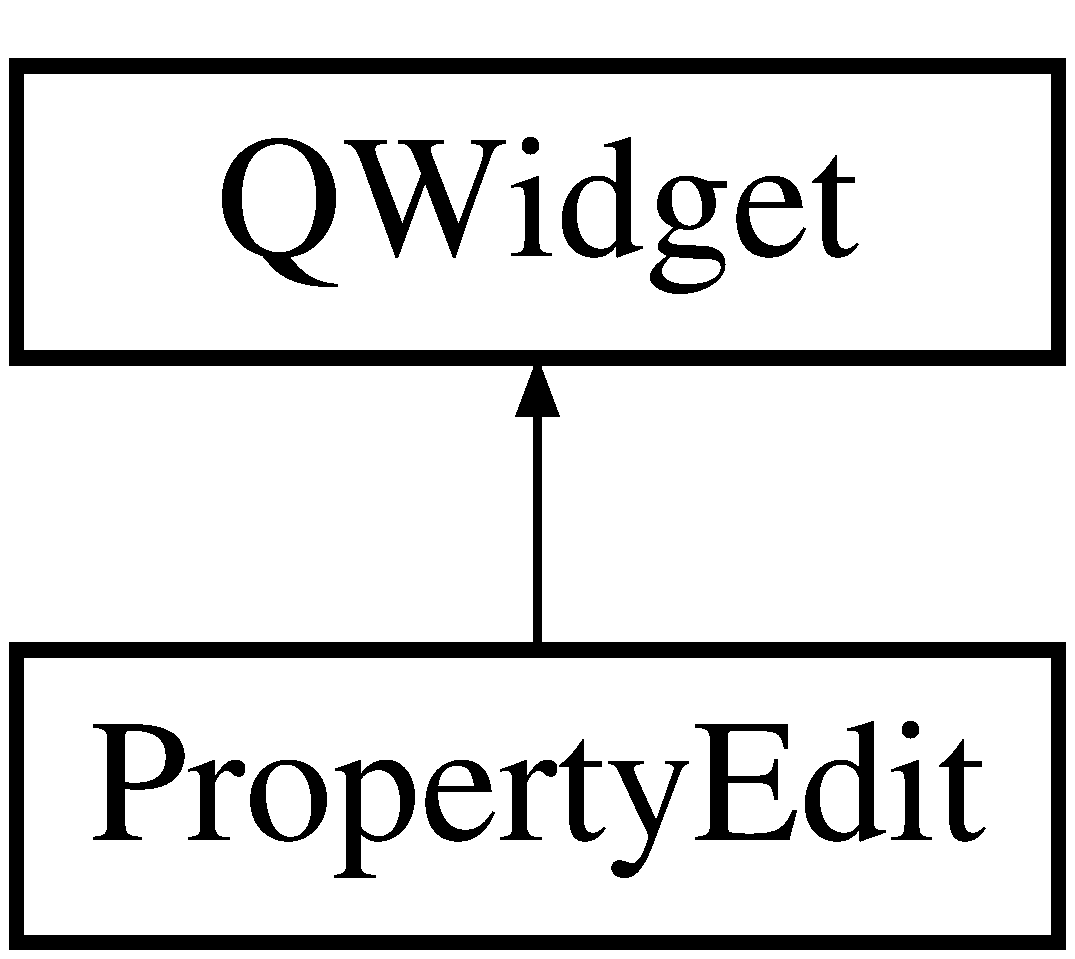
\includegraphics[height=2.000000cm]{class_property_edit}
\end{center}
\end{figure}
\subsection*{Public Member Functions}
\begin{DoxyCompactItemize}
\item 
\mbox{\Hypertarget{class_property_edit_a9faa7e41a8409ccc727d8c96e92e86e5}\label{class_property_edit_a9faa7e41a8409ccc727d8c96e92e86e5}} 
{\bfseries Property\+Edit} (const Q\+Json\+Object \&config, Q\+Widget $\ast$parent=Q\+\_\+\+N\+U\+L\+L\+P\+TR)
\item 
Q\+Json\+Object \mbox{\hyperlink{class_property_edit_a94cdfb72670c88ca66a29b4a62632c8a}{to\+Json}} () const
\begin{DoxyCompactList}\small\item\em Returns a json object of the components values. \end{DoxyCompactList}\item 
void \mbox{\hyperlink{class_property_edit_a5c708a29919c4452d7f34321f38a572e}{from\+Json}} (const Q\+Json\+Object \&values)
\begin{DoxyCompactList}\small\item\em Initializes the component from json configuration. \end{DoxyCompactList}\item 
Q\+String \mbox{\hyperlink{class_property_edit_a44ce9e0c1a30c7d6a2819740613d05c0}{get\+Attribute}} () const
\begin{DoxyCompactList}\small\item\em Returns the attribute set in the ui configuraion. \end{DoxyCompactList}\end{DoxyCompactItemize}


\subsection{Detailed Description}
The \mbox{\hyperlink{class_property_edit}{Property\+Edit}} class creates a specified amount of Q\+Spinboxes as well as a Label naming the properties they change. 

Details on the configuraion structure can be found within the \mbox{\hyperlink{class_configurator}{Configurator}} class. 

\subsection{Member Function Documentation}
\mbox{\Hypertarget{class_property_edit_a5c708a29919c4452d7f34321f38a572e}\label{class_property_edit_a5c708a29919c4452d7f34321f38a572e}} 
\index{Property\+Edit@{Property\+Edit}!from\+Json@{from\+Json}}
\index{from\+Json@{from\+Json}!Property\+Edit@{Property\+Edit}}
\subsubsection{\texorpdfstring{from\+Json()}{fromJson()}}
{\footnotesize\ttfamily void Property\+Edit\+::from\+Json (\begin{DoxyParamCaption}\item[{const Q\+Json\+Object \&}]{values }\end{DoxyParamCaption})}



Initializes the component from json configuration. 


\begin{DoxyParams}{Parameters}
{\em values} & \\
\hline
\end{DoxyParams}
\mbox{\Hypertarget{class_property_edit_a44ce9e0c1a30c7d6a2819740613d05c0}\label{class_property_edit_a44ce9e0c1a30c7d6a2819740613d05c0}} 
\index{Property\+Edit@{Property\+Edit}!get\+Attribute@{get\+Attribute}}
\index{get\+Attribute@{get\+Attribute}!Property\+Edit@{Property\+Edit}}
\subsubsection{\texorpdfstring{get\+Attribute()}{getAttribute()}}
{\footnotesize\ttfamily Q\+String Property\+Edit\+::get\+Attribute (\begin{DoxyParamCaption}{ }\end{DoxyParamCaption}) const}



Returns the attribute set in the ui configuraion. 

\begin{DoxyReturn}{Returns}

\end{DoxyReturn}
\mbox{\Hypertarget{class_property_edit_a94cdfb72670c88ca66a29b4a62632c8a}\label{class_property_edit_a94cdfb72670c88ca66a29b4a62632c8a}} 
\index{Property\+Edit@{Property\+Edit}!to\+Json@{to\+Json}}
\index{to\+Json@{to\+Json}!Property\+Edit@{Property\+Edit}}
\subsubsection{\texorpdfstring{to\+Json()}{toJson()}}
{\footnotesize\ttfamily Q\+Json\+Object Property\+Edit\+::to\+Json (\begin{DoxyParamCaption}{ }\end{DoxyParamCaption}) const}



Returns a json object of the components values. 

\begin{DoxyReturn}{Returns}
Q\+Json\+Object containing the set value 
\end{DoxyReturn}


The documentation for this class was generated from the following files\+:\begin{DoxyCompactItemize}
\item 
/\+Users/h\+Gen/\+Desktop/qt/glwarp-\/configuration-\/tool/src/ui/propertyedit.\+hpp\item 
/\+Users/h\+Gen/\+Desktop/qt/glwarp-\/configuration-\/tool/src/ui/propertyedit.\+cpp\end{DoxyCompactItemize}

\hypertarget{class_property_edit_group}{}\section{Property\+Edit\+Group Class Reference}
\label{class_property_edit_group}\index{Property\+Edit\+Group@{Property\+Edit\+Group}}


The \mbox{\hyperlink{class_property_edit_group}{Property\+Edit\+Group}} class wraps n Property\+Edits according to the specifies configuration.  




{\ttfamily \#include $<$propertyeditgroup.\+h$>$}

Inheritance diagram for Property\+Edit\+Group\+:\begin{figure}[H]
\begin{center}
\leavevmode
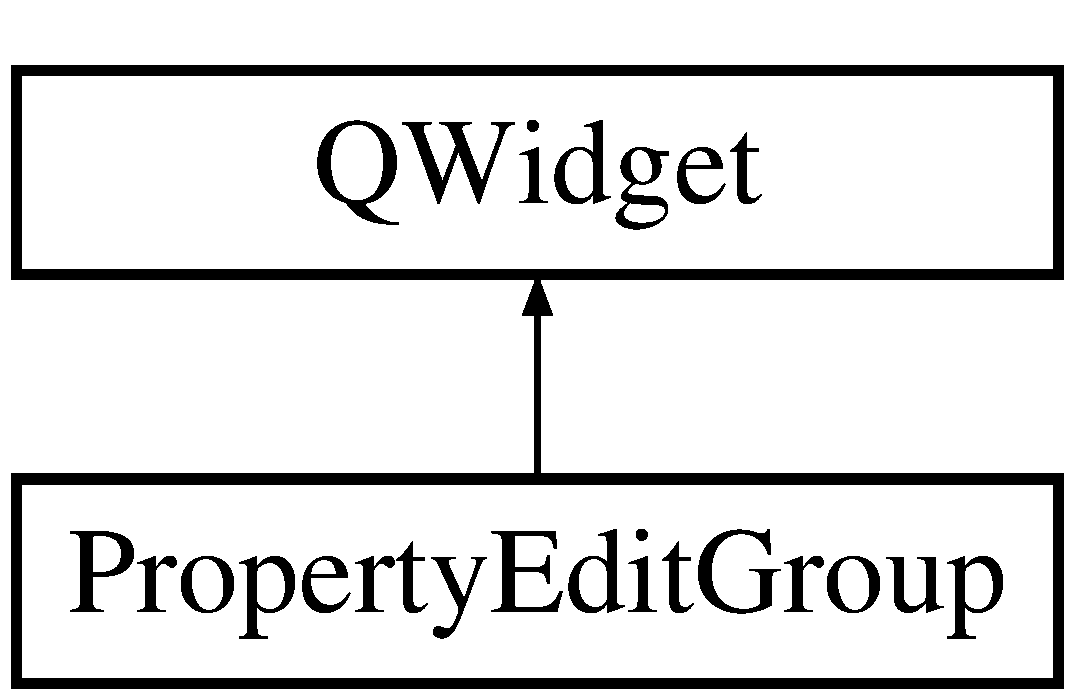
\includegraphics[height=2.000000cm]{class_property_edit_group}
\end{center}
\end{figure}
\subsection*{Public Member Functions}
\begin{DoxyCompactItemize}
\item 
\mbox{\Hypertarget{class_property_edit_group_a18e370044e616ade52f31ba90cc9652c}\label{class_property_edit_group_a18e370044e616ade52f31ba90cc9652c}} 
{\bfseries Property\+Edit\+Group} (const Q\+Json\+Object \&config, Q\+Widget $\ast$parent=Q\+\_\+\+N\+U\+L\+L\+P\+TR)
\item 
Q\+Json\+Object \mbox{\hyperlink{class_property_edit_group_a8465118b18404dc711408268f992dc67}{to\+Json}} () const
\begin{DoxyCompactList}\small\item\em Returns json containing values of all child elements. \end{DoxyCompactList}\item 
void \mbox{\hyperlink{class_property_edit_group_ab67d4c9653391c01be0a094dcf33f750}{from\+Json}} (const Q\+Json\+Object \&values)
\begin{DoxyCompactList}\small\item\em Set child values from Json. \end{DoxyCompactList}\item 
Q\+String \mbox{\hyperlink{class_property_edit_group_a1f29d82fefe5673830f941dc88a9fca3}{get\+Attribute}} () const
\begin{DoxyCompactList}\small\item\em Returns groups attribute. \end{DoxyCompactList}\end{DoxyCompactItemize}


\subsection{Detailed Description}
The \mbox{\hyperlink{class_property_edit_group}{Property\+Edit\+Group}} class wraps n Property\+Edits according to the specifies configuration. 

Details on the configuraion structure can be found within the \mbox{\hyperlink{class_configurator}{Configurator}} class 

\subsection{Member Function Documentation}
\mbox{\Hypertarget{class_property_edit_group_ab67d4c9653391c01be0a094dcf33f750}\label{class_property_edit_group_ab67d4c9653391c01be0a094dcf33f750}} 
\index{Property\+Edit\+Group@{Property\+Edit\+Group}!from\+Json@{from\+Json}}
\index{from\+Json@{from\+Json}!Property\+Edit\+Group@{Property\+Edit\+Group}}
\subsubsection{\texorpdfstring{from\+Json()}{fromJson()}}
{\footnotesize\ttfamily void Property\+Edit\+Group\+::from\+Json (\begin{DoxyParamCaption}\item[{const Q\+Json\+Object \&}]{values }\end{DoxyParamCaption})}



Set child values from Json. 


\begin{DoxyParams}{Parameters}
{\em values} & \\
\hline
\end{DoxyParams}
\mbox{\Hypertarget{class_property_edit_group_a1f29d82fefe5673830f941dc88a9fca3}\label{class_property_edit_group_a1f29d82fefe5673830f941dc88a9fca3}} 
\index{Property\+Edit\+Group@{Property\+Edit\+Group}!get\+Attribute@{get\+Attribute}}
\index{get\+Attribute@{get\+Attribute}!Property\+Edit\+Group@{Property\+Edit\+Group}}
\subsubsection{\texorpdfstring{get\+Attribute()}{getAttribute()}}
{\footnotesize\ttfamily Q\+String Property\+Edit\+Group\+::get\+Attribute (\begin{DoxyParamCaption}{ }\end{DoxyParamCaption}) const}



Returns groups attribute. 

\begin{DoxyReturn}{Returns}

\end{DoxyReturn}
\mbox{\Hypertarget{class_property_edit_group_a8465118b18404dc711408268f992dc67}\label{class_property_edit_group_a8465118b18404dc711408268f992dc67}} 
\index{Property\+Edit\+Group@{Property\+Edit\+Group}!to\+Json@{to\+Json}}
\index{to\+Json@{to\+Json}!Property\+Edit\+Group@{Property\+Edit\+Group}}
\subsubsection{\texorpdfstring{to\+Json()}{toJson()}}
{\footnotesize\ttfamily Q\+Json\+Object Property\+Edit\+Group\+::to\+Json (\begin{DoxyParamCaption}{ }\end{DoxyParamCaption}) const}



Returns json containing values of all child elements. 

\begin{DoxyReturn}{Returns}

\end{DoxyReturn}


The documentation for this class was generated from the following files\+:\begin{DoxyCompactItemize}
\item 
/\+Users/h\+Gen/\+Desktop/qt/glwarp-\/configuration-\/tool/src/ui/propertyeditgroup.\+h\item 
/\+Users/h\+Gen/\+Desktop/qt/glwarp-\/configuration-\/tool/src/ui/propertyeditgroup.\+cpp\end{DoxyCompactItemize}

\hypertarget{struct_ray}{}\section{Ray Struct Reference}
\label{struct_ray}\index{Ray@{Ray}}


The \mbox{\hyperlink{struct_ray}{Ray}} struct describes a ray that can be cast from an origin towards a specified direction.  




{\ttfamily \#include $<$ray.\+hpp$>$}

\subsection*{Public Member Functions}
\begin{DoxyCompactItemize}
\item 
\mbox{\hyperlink{struct_ray_a2e3d2c29f2df4ab3da10da79d4acb852}{Ray}} ()
\item 
\mbox{\hyperlink{struct_ray_a92effebbda59de6b4f889718dec7520a}{Ray}} (const Q\+Vector3D \&origin)
\item 
\mbox{\hyperlink{struct_ray_a46a83135920eb622d6c51cc15091c6fc}{Ray}} (const Q\+Vector3D \&origin, const Q\+Vector3D \&direction)
\item 
\mbox{\hyperlink{struct_ray_a155a0b6573cf6a9a2256eb5062523daf}{Ray}} (const \mbox{\hyperlink{struct_ray}{Ray}} \&ray)
\item 
\mbox{\hyperlink{struct_ray_a8b0e575ce5df046c0c7615c32a96a46f}{$\sim$\+Ray}} ()
\item 
Q\+Vector3D \mbox{\hyperlink{struct_ray_aaa4b1d97ddd42e6a4a880b0854f0e84e}{reflect}} (Q\+Vector3D const \&normal) const
\begin{DoxyCompactList}\small\item\em Returns the reflection vector of this ray with a specified normal. \end{DoxyCompactList}\end{DoxyCompactItemize}
\subsection*{Public Attributes}
\begin{DoxyCompactItemize}
\item 
\mbox{\Hypertarget{struct_ray_a8e3059d44fffe72fb98bb23528016a74}\label{struct_ray_a8e3059d44fffe72fb98bb23528016a74}} 
Q\+Vector3D {\bfseries origin}
\item 
\mbox{\Hypertarget{struct_ray_a4480e81172e55beea90f19542bb35fa4}\label{struct_ray_a4480e81172e55beea90f19542bb35fa4}} 
Q\+Vector3D {\bfseries direction}
\end{DoxyCompactItemize}
\subsection*{Friends}
\begin{DoxyCompactItemize}
\item 
std\+::ostream \& \mbox{\hyperlink{struct_ray_a5c8a3bf0a8e125a67943f442cbbf8e06}{operator$<$$<$}} (std\+::ostream \&os, const \mbox{\hyperlink{struct_ray}{Ray}} \&ray)
\begin{DoxyCompactList}\small\item\em operator $<$$<$ used for printing the Class using std$<$$<$cout; \end{DoxyCompactList}\end{DoxyCompactItemize}


\subsection{Detailed Description}
The \mbox{\hyperlink{struct_ray}{Ray}} struct describes a ray that can be cast from an origin towards a specified direction. 

\subsection{Constructor \& Destructor Documentation}
\mbox{\Hypertarget{struct_ray_a2e3d2c29f2df4ab3da10da79d4acb852}\label{struct_ray_a2e3d2c29f2df4ab3da10da79d4acb852}} 
\index{Ray@{Ray}!Ray@{Ray}}
\index{Ray@{Ray}!Ray@{Ray}}
\subsubsection{\texorpdfstring{Ray()}{Ray()}\hspace{0.1cm}{\footnotesize\ttfamily [1/4]}}
{\footnotesize\ttfamily Ray\+::\+Ray (\begin{DoxyParamCaption}{ }\end{DoxyParamCaption})}

default c\textquotesingle{}tor \mbox{\Hypertarget{struct_ray_a92effebbda59de6b4f889718dec7520a}\label{struct_ray_a92effebbda59de6b4f889718dec7520a}} 
\index{Ray@{Ray}!Ray@{Ray}}
\index{Ray@{Ray}!Ray@{Ray}}
\subsubsection{\texorpdfstring{Ray()}{Ray()}\hspace{0.1cm}{\footnotesize\ttfamily [2/4]}}
{\footnotesize\ttfamily Ray\+::\+Ray (\begin{DoxyParamCaption}\item[{const Q\+Vector3D \&}]{origin }\end{DoxyParamCaption})}

c\textquotesingle{}tor 
\begin{DoxyParams}{Parameters}
{\em origin} & \\
\hline
\end{DoxyParams}
\mbox{\Hypertarget{struct_ray_a46a83135920eb622d6c51cc15091c6fc}\label{struct_ray_a46a83135920eb622d6c51cc15091c6fc}} 
\index{Ray@{Ray}!Ray@{Ray}}
\index{Ray@{Ray}!Ray@{Ray}}
\subsubsection{\texorpdfstring{Ray()}{Ray()}\hspace{0.1cm}{\footnotesize\ttfamily [3/4]}}
{\footnotesize\ttfamily Ray\+::\+Ray (\begin{DoxyParamCaption}\item[{const Q\+Vector3D \&}]{origin,  }\item[{const Q\+Vector3D \&}]{direction }\end{DoxyParamCaption})}

c\textquotesingle{}tor 
\begin{DoxyParams}{Parameters}
{\em origin} & \\
\hline
{\em direction} & \\
\hline
\end{DoxyParams}
\mbox{\Hypertarget{struct_ray_a155a0b6573cf6a9a2256eb5062523daf}\label{struct_ray_a155a0b6573cf6a9a2256eb5062523daf}} 
\index{Ray@{Ray}!Ray@{Ray}}
\index{Ray@{Ray}!Ray@{Ray}}
\subsubsection{\texorpdfstring{Ray()}{Ray()}\hspace{0.1cm}{\footnotesize\ttfamily [4/4]}}
{\footnotesize\ttfamily Ray\+::\+Ray (\begin{DoxyParamCaption}\item[{const \mbox{\hyperlink{struct_ray}{Ray}} \&}]{ray }\end{DoxyParamCaption})}

copy c\textquotesingle{}tor 
\begin{DoxyParams}{Parameters}
{\em ray} & \\
\hline
\end{DoxyParams}
\mbox{\Hypertarget{struct_ray_a8b0e575ce5df046c0c7615c32a96a46f}\label{struct_ray_a8b0e575ce5df046c0c7615c32a96a46f}} 
\index{Ray@{Ray}!````~Ray@{$\sim$\+Ray}}
\index{````~Ray@{$\sim$\+Ray}!Ray@{Ray}}
\subsubsection{\texorpdfstring{$\sim$\+Ray()}{~Ray()}}
{\footnotesize\ttfamily Ray\+::$\sim$\+Ray (\begin{DoxyParamCaption}{ }\end{DoxyParamCaption})}

d\textquotesingle{}tor 

\subsection{Member Function Documentation}
\mbox{\Hypertarget{struct_ray_aaa4b1d97ddd42e6a4a880b0854f0e84e}\label{struct_ray_aaa4b1d97ddd42e6a4a880b0854f0e84e}} 
\index{Ray@{Ray}!reflect@{reflect}}
\index{reflect@{reflect}!Ray@{Ray}}
\subsubsection{\texorpdfstring{reflect()}{reflect()}}
{\footnotesize\ttfamily Q\+Vector3D Ray\+::reflect (\begin{DoxyParamCaption}\item[{Q\+Vector3D const \&}]{hitpoint\+\_\+normal }\end{DoxyParamCaption}) const}



Returns the reflection vector of this ray with a specified normal. 


\begin{DoxyParams}{Parameters}
{\em normal} & \\
\hline
\end{DoxyParams}
\begin{DoxyReturn}{Returns}

\end{DoxyReturn}
reflect ray along given normal 
\begin{DoxyParams}{Parameters}
{\em normal} & \\
\hline
\end{DoxyParams}
\begin{DoxyReturn}{Returns}

\end{DoxyReturn}


\subsection{Friends And Related Function Documentation}
\mbox{\Hypertarget{struct_ray_a5c8a3bf0a8e125a67943f442cbbf8e06}\label{struct_ray_a5c8a3bf0a8e125a67943f442cbbf8e06}} 
\index{Ray@{Ray}!operator$<$$<$@{operator$<$$<$}}
\index{operator$<$$<$@{operator$<$$<$}!Ray@{Ray}}
\subsubsection{\texorpdfstring{operator$<$$<$}{operator<<}}
{\footnotesize\ttfamily std\+::ostream\& operator$<$$<$ (\begin{DoxyParamCaption}\item[{std\+::ostream \&}]{os,  }\item[{const \mbox{\hyperlink{struct_ray}{Ray}} \&}]{ray }\end{DoxyParamCaption})\hspace{0.3cm}{\ttfamily [friend]}}



operator $<$$<$ used for printing the Class using std$<$$<$cout; 

Because of reasons, Qt has its own way of printing things. Therefor this\textquotesingle{}ll not work with Qt\textquotesingle{}s q\+Debug() $<$$<$

I\textquotesingle{}m not going to look into this, ... just because.


\begin{DoxyParams}{Parameters}
{\em os} & \\
\hline
{\em ray} & \\
\hline
\end{DoxyParams}
\begin{DoxyReturn}{Returns}

\end{DoxyReturn}
stream $<$$<$ output operator 
\begin{DoxyParams}{Parameters}
{\em os} & \\
\hline
{\em ray} & \\
\hline
\end{DoxyParams}
\begin{DoxyReturn}{Returns}

\end{DoxyReturn}


The documentation for this struct was generated from the following files\+:\begin{DoxyCompactItemize}
\item 
/\+Users/h\+Gen/\+Desktop/qt/glwarp-\/configuration-\/tool/src/model/ray.\+hpp\item 
/\+Users/h\+Gen/\+Desktop/qt/glwarp-\/configuration-\/tool/src/model/ray.\+cpp\end{DoxyCompactItemize}

\hypertarget{class_scene}{}\section{Scene Struct Reference}
\label{class_scene}\index{Scene@{Scene}}


The \mbox{\hyperlink{class_scene}{Scene}} struct contains all values needed by the Gl\+Widget class to render a simulated configuration.  




{\ttfamily \#include $<$simulation.\+h$>$}

\subsection*{Public Attributes}
\begin{DoxyCompactItemize}
\item 
\mbox{\Hypertarget{class_scene_ac73d19d8cf3309348b3302c607404b73}\label{class_scene_ac73d19d8cf3309348b3302c607404b73}} 
std\+::vector$<$ Q\+Vector3D $>$ {\bfseries sample\+\_\+grid}
\item 
\mbox{\Hypertarget{class_scene_ae9ef639317ddd27e4073a33b23e62810}\label{class_scene_ae9ef639317ddd27e4073a33b23e62810}} 
std\+::vector$<$ Q\+Vector3D $>$ {\bfseries first\+\_\+hits}
\item 
\mbox{\Hypertarget{class_scene_acff925f0a3de398bcbeca5f51a32395c}\label{class_scene_acff925f0a3de398bcbeca5f51a32395c}} 
std\+::vector$<$ Q\+Vector3D $>$ {\bfseries second\+\_\+hits}
\item 
\mbox{\Hypertarget{class_scene_aed6376924dbd14c550452dc9c8ba0341}\label{class_scene_aed6376924dbd14c550452dc9c8ba0341}} 
std\+::vector$<$ Q\+Vector3D $>$ {\bfseries dome\+\_\+vertices}
\item 
\mbox{\Hypertarget{class_scene_a594e36de7f91ec97a3e9d08e05a339af}\label{class_scene_a594e36de7f91ec97a3e9d08e05a339af}} 
std\+::vector$<$ Q\+Vector3D $>$ {\bfseries screen\+\_\+points}
\item 
\mbox{\Hypertarget{class_scene_a6aacb490dbf456d4c5c4b6099aa10170}\label{class_scene_a6aacb490dbf456d4c5c4b6099aa10170}} 
std\+::vector$<$ Q\+Vector3D $>$ {\bfseries texture\+\_\+coords}
\item 
\mbox{\Hypertarget{class_scene_a06d1a5251c4f51f8713be41c1a4cda1e}\label{class_scene_a06d1a5251c4f51f8713be41c1a4cda1e}} 
std\+::map$<$ Projector\+Frustum\+::\+Corner, Q\+Vector3D $>$ {\bfseries near\+\_\+corners}
\item 
\mbox{\Hypertarget{class_scene_a11c304f37b7373f14cf95e19a4b52c7b}\label{class_scene_a11c304f37b7373f14cf95e19a4b52c7b}} 
std\+::map$<$ Projector\+Frustum\+::\+Corner, Q\+Vector3D $>$ {\bfseries far\+\_\+corners}
\end{DoxyCompactItemize}


\subsection{Detailed Description}
The \mbox{\hyperlink{class_scene}{Scene}} struct contains all values needed by the Gl\+Widget class to render a simulated configuration. 

The documentation for this struct was generated from the following files\+:\begin{DoxyCompactItemize}
\item 
/\+Users/h\+Gen/\+Desktop/qt/glwarp-\/configuration-\/tool/src/model/scene.\+h\item 
/\+Users/h\+Gen/\+Desktop/qt/glwarp-\/configuration-\/tool/src/model/simulation.\+h\item 
/\+Users/h\+Gen/\+Desktop/qt/glwarp-\/configuration-\/tool/src/model/scene.\+cpp\end{DoxyCompactItemize}

\hypertarget{class_simulation}{}\section{Simulation Class Reference}
\label{class_simulation}\index{Simulation@{Simulation}}


The \mbox{\hyperlink{class_simulation}{Simulation}} class handles single model simulation passes. The \mbox{\hyperlink{class_simulation}{Simulation}} is a mere middleman handling connections to the model from the outside as well as passing computed results to outter classes and interfaces.  




{\ttfamily \#include $<$simulation.\+h$>$}

\subsection*{Public Member Functions}
\begin{DoxyCompactItemize}
\item 
\mbox{\Hypertarget{class_simulation_afd97d61478060a4cc1bd7470f6c865aa}\label{class_simulation_afd97d61478060a4cc1bd7470f6c865aa}} 
void \mbox{\hyperlink{class_simulation_afd97d61478060a4cc1bd7470f6c865aa}{run\+Calculations}} ()
\begin{DoxyCompactList}\small\item\em Runs a \mbox{\hyperlink{class_simulation}{Simulation}} pass. \end{DoxyCompactList}\item 
void \mbox{\hyperlink{class_simulation_a9cb0aae7c447fd77c0dd7900e925e03e}{initialize}} (\mbox{\hyperlink{struct_model_config}{Model\+Config}} $\ast$model\+\_\+config)
\begin{DoxyCompactList}\small\item\em Initializes main \mbox{\hyperlink{class_simulation}{Simulation}} components. \end{DoxyCompactList}\item 
void \mbox{\hyperlink{class_simulation_a0a19a19f99d3e88f020c8e1a4b7d8440}{update\+From\+Config}} (\mbox{\hyperlink{struct_model_config}{Model\+Config}} $\ast$model\+\_\+config)
\begin{DoxyCompactList}\small\item\em Updates the \mbox{\hyperlink{class_simulation}{Simulation}} from given json configuration. \end{DoxyCompactList}\item 
void \mbox{\hyperlink{class_simulation_a6b801c919ee95c0d967a8037cd73afe5}{build\+Model}} (\mbox{\hyperlink{struct_model_config}{Model\+Config}} $\ast$model\+\_\+config)
\begin{DoxyCompactList}\small\item\em Builds the model. \end{DoxyCompactList}\item 
\mbox{\Hypertarget{class_simulation_ad9bd99eb4bc5bb719f7a9a7abe377b49}\label{class_simulation_ad9bd99eb4bc5bb719f7a9a7abe377b49}} 
\mbox{\hyperlink{class_scene}{Scene}} \mbox{\hyperlink{class_simulation_ad9bd99eb4bc5bb719f7a9a7abe377b49}{get\+Current\+Scene}} () const
\begin{DoxyCompactList}\small\item\em Returns a scene dto. \end{DoxyCompactList}\item 
std\+::vector$<$ Q\+Vector3D $>$ \mbox{\hyperlink{class_simulation_a51325a28f5c8d5e37cb8d90fb6f79634}{get\+Transformation\+Mesh}} () const
\begin{DoxyCompactList}\small\item\em Returns the current transformation mesh points. \end{DoxyCompactList}\item 
std\+::vector$<$ Q\+Vector3D $>$ \mbox{\hyperlink{class_simulation_a7dfcbd7e6fe8e6c1c57e01f8367da642}{get\+Texture\+Coords}} () const
\begin{DoxyCompactList}\small\item\em Returns the current calculated texture coordinates. \end{DoxyCompactList}\end{DoxyCompactItemize}


\subsection{Detailed Description}
The \mbox{\hyperlink{class_simulation}{Simulation}} class handles single model simulation passes. The \mbox{\hyperlink{class_simulation}{Simulation}} is a mere middleman handling connections to the model from the outside as well as passing computed results to outter classes and interfaces. 

\subsection{Member Function Documentation}
\mbox{\Hypertarget{class_simulation_a6b801c919ee95c0d967a8037cd73afe5}\label{class_simulation_a6b801c919ee95c0d967a8037cd73afe5}} 
\index{Simulation@{Simulation}!build\+Model@{build\+Model}}
\index{build\+Model@{build\+Model}!Simulation@{Simulation}}
\subsubsection{\texorpdfstring{build\+Model()}{buildModel()}}
{\footnotesize\ttfamily void Simulation\+::build\+Model (\begin{DoxyParamCaption}\item[{\mbox{\hyperlink{struct_model_config}{Model\+Config}} $\ast$}]{model\+\_\+config }\end{DoxyParamCaption})}



Builds the model. 


\begin{DoxyParams}{Parameters}
{\em model\+\_\+config} & \\
\hline
\end{DoxyParams}
\mbox{\Hypertarget{class_simulation_a7dfcbd7e6fe8e6c1c57e01f8367da642}\label{class_simulation_a7dfcbd7e6fe8e6c1c57e01f8367da642}} 
\index{Simulation@{Simulation}!get\+Texture\+Coords@{get\+Texture\+Coords}}
\index{get\+Texture\+Coords@{get\+Texture\+Coords}!Simulation@{Simulation}}
\subsubsection{\texorpdfstring{get\+Texture\+Coords()}{getTextureCoords()}}
{\footnotesize\ttfamily std\+::vector$<$ Q\+Vector3D $>$ Simulation\+::get\+Texture\+Coords (\begin{DoxyParamCaption}{ }\end{DoxyParamCaption}) const}



Returns the current calculated texture coordinates. 

\begin{DoxyReturn}{Returns}

\end{DoxyReturn}
\mbox{\Hypertarget{class_simulation_a51325a28f5c8d5e37cb8d90fb6f79634}\label{class_simulation_a51325a28f5c8d5e37cb8d90fb6f79634}} 
\index{Simulation@{Simulation}!get\+Transformation\+Mesh@{get\+Transformation\+Mesh}}
\index{get\+Transformation\+Mesh@{get\+Transformation\+Mesh}!Simulation@{Simulation}}
\subsubsection{\texorpdfstring{get\+Transformation\+Mesh()}{getTransformationMesh()}}
{\footnotesize\ttfamily std\+::vector$<$ Q\+Vector3D $>$ Simulation\+::get\+Transformation\+Mesh (\begin{DoxyParamCaption}{ }\end{DoxyParamCaption}) const}



Returns the current transformation mesh points. 

\begin{DoxyReturn}{Returns}

\end{DoxyReturn}
\mbox{\Hypertarget{class_simulation_a9cb0aae7c447fd77c0dd7900e925e03e}\label{class_simulation_a9cb0aae7c447fd77c0dd7900e925e03e}} 
\index{Simulation@{Simulation}!initialize@{initialize}}
\index{initialize@{initialize}!Simulation@{Simulation}}
\subsubsection{\texorpdfstring{initialize()}{initialize()}}
{\footnotesize\ttfamily void Simulation\+::initialize (\begin{DoxyParamCaption}\item[{\mbox{\hyperlink{struct_model_config}{Model\+Config}} $\ast$}]{model\+\_\+config }\end{DoxyParamCaption})}



Initializes main \mbox{\hyperlink{class_simulation}{Simulation}} components. 

Components created are\+: the first reflection mirror $<$\+Sphere$>$ the final reflection medium $<$\+Sphere$>$ the dome projector maintaining the calculations $<$\+Dome\+Projector$>$


\begin{DoxyParams}{Parameters}
{\em model\+\_\+config} & \\
\hline
\end{DoxyParams}
\mbox{\Hypertarget{class_simulation_a0a19a19f99d3e88f020c8e1a4b7d8440}\label{class_simulation_a0a19a19f99d3e88f020c8e1a4b7d8440}} 
\index{Simulation@{Simulation}!update\+From\+Config@{update\+From\+Config}}
\index{update\+From\+Config@{update\+From\+Config}!Simulation@{Simulation}}
\subsubsection{\texorpdfstring{update\+From\+Config()}{updateFromConfig()}}
{\footnotesize\ttfamily void Simulation\+::update\+From\+Config (\begin{DoxyParamCaption}\item[{\mbox{\hyperlink{struct_model_config}{Model\+Config}} $\ast$}]{model\+\_\+config }\end{DoxyParamCaption})}



Updates the \mbox{\hyperlink{class_simulation}{Simulation}} from given json configuration. 


\begin{DoxyParams}{Parameters}
{\em config} & \\
\hline
\end{DoxyParams}


The documentation for this class was generated from the following files\+:\begin{DoxyCompactItemize}
\item 
/\+Users/h\+Gen/\+Desktop/qt/glwarp-\/configuration-\/tool/src/model/simulation.\+h\item 
/\+Users/h\+Gen/\+Desktop/qt/glwarp-\/configuration-\/tool/src/model/simulation.\+cpp\end{DoxyCompactItemize}

\hypertarget{class_sphere}{}\section{Sphere Class Reference}
\label{class_sphere}\index{Sphere@{Sphere}}
\subsection*{Public Member Functions}
\begin{DoxyCompactItemize}
\item 
\mbox{\Hypertarget{class_sphere_a890a63ff583cb88e7ec4e840b4ef5eb9}\label{class_sphere_a890a63ff583cb88e7ec4e840b4ef5eb9}} 
\mbox{\hyperlink{class_sphere_a890a63ff583cb88e7ec4e840b4ef5eb9}{Sphere}} ()
\begin{DoxyCompactList}\small\item\em \mbox{\hyperlink{class_sphere}{Sphere}} c\textquotesingle{}tor. \end{DoxyCompactList}\item 
\mbox{\Hypertarget{class_sphere_a066dd77d24d95f7cb2e16880b3a5ae6e}\label{class_sphere_a066dd77d24d95f7cb2e16880b3a5ae6e}} 
\mbox{\hyperlink{class_sphere_a066dd77d24d95f7cb2e16880b3a5ae6e}{Sphere}} (float radius)
\begin{DoxyCompactList}\small\item\em \mbox{\hyperlink{class_sphere}{Sphere}}. \end{DoxyCompactList}\item 
\mbox{\hyperlink{class_sphere_a507519d4ee1d48277626fe3c74e8228b}{Sphere}} (float radius, const Q\+Vector3D \&position)
\begin{DoxyCompactList}\small\item\em \mbox{\hyperlink{class_sphere}{Sphere}}. \end{DoxyCompactList}\item 
bool \mbox{\hyperlink{class_sphere_a789d83c264bed2ee64a30bca1261ab41}{intersect}} (\mbox{\hyperlink{struct_ray}{Ray}} const \&r, std\+::pair$<$ \mbox{\hyperlink{struct_hitpoint}{Hitpoint}}, \mbox{\hyperlink{struct_hitpoint}{Hitpoint}} $>$ $\ast$hp\+\_\+pair)
\item 
float \mbox{\hyperlink{class_sphere_ac22727cc5f7fdac7548798fb88f7cadd}{get\+\_\+radius}} () const
\begin{DoxyCompactList}\small\item\em Returns the spheres radius. \end{DoxyCompactList}\item 
Q\+Vector3D \mbox{\hyperlink{class_sphere_a253bd3ccf57e854989fb49c835fddb0b}{get\+\_\+position}} () const
\begin{DoxyCompactList}\small\item\em Returns the spheres position. \end{DoxyCompactList}\item 
void \mbox{\hyperlink{class_sphere_ad050355312225f312b676edc376158e1}{set\+\_\+position}} (const Q\+Vector3D \&new\+\_\+position)
\begin{DoxyCompactList}\small\item\em Set the Spheres position. \end{DoxyCompactList}\item 
void \mbox{\hyperlink{class_sphere_a293cdd84dea67955c6a7d14e86c8d919}{set\+\_\+radius}} (float new\+\_\+radius)
\begin{DoxyCompactList}\small\item\em Set the Spheres radius. \end{DoxyCompactList}\end{DoxyCompactItemize}
\subsection*{Friends}
\begin{DoxyCompactItemize}
\item 
std\+::ostream \& \mbox{\hyperlink{class_sphere_adeb07662f568bb893f87459c082f00b2}{operator$<$$<$}} (std\+::ostream \&os, const \mbox{\hyperlink{class_sphere}{Sphere}} \&sphere)
\begin{DoxyCompactList}\small\item\em operator $<$$<$ used for printing the Class using std$<$$<$cout; \end{DoxyCompactList}\end{DoxyCompactItemize}


\subsection{Constructor \& Destructor Documentation}
\mbox{\Hypertarget{class_sphere_a507519d4ee1d48277626fe3c74e8228b}\label{class_sphere_a507519d4ee1d48277626fe3c74e8228b}} 
\index{Sphere@{Sphere}!Sphere@{Sphere}}
\index{Sphere@{Sphere}!Sphere@{Sphere}}
\subsubsection{\texorpdfstring{Sphere()}{Sphere()}}
{\footnotesize\ttfamily Sphere\+::\+Sphere (\begin{DoxyParamCaption}\item[{float}]{radius,  }\item[{const Q\+Vector3D \&}]{position }\end{DoxyParamCaption})}



\mbox{\hyperlink{class_sphere}{Sphere}}. 


\begin{DoxyParams}{Parameters}
{\em radius} & \\
\hline
{\em position} & \\
\hline
\end{DoxyParams}


\subsection{Member Function Documentation}
\mbox{\Hypertarget{class_sphere_a253bd3ccf57e854989fb49c835fddb0b}\label{class_sphere_a253bd3ccf57e854989fb49c835fddb0b}} 
\index{Sphere@{Sphere}!get\+\_\+position@{get\+\_\+position}}
\index{get\+\_\+position@{get\+\_\+position}!Sphere@{Sphere}}
\subsubsection{\texorpdfstring{get\+\_\+position()}{get\_position()}}
{\footnotesize\ttfamily Q\+Vector3D Sphere\+::get\+\_\+position (\begin{DoxyParamCaption}{ }\end{DoxyParamCaption}) const}



Returns the spheres position. 

\begin{DoxyReturn}{Returns}

\end{DoxyReturn}
\mbox{\Hypertarget{class_sphere_ac22727cc5f7fdac7548798fb88f7cadd}\label{class_sphere_ac22727cc5f7fdac7548798fb88f7cadd}} 
\index{Sphere@{Sphere}!get\+\_\+radius@{get\+\_\+radius}}
\index{get\+\_\+radius@{get\+\_\+radius}!Sphere@{Sphere}}
\subsubsection{\texorpdfstring{get\+\_\+radius()}{get\_radius()}}
{\footnotesize\ttfamily float Sphere\+::get\+\_\+radius (\begin{DoxyParamCaption}{ }\end{DoxyParamCaption}) const}



Returns the spheres radius. 

\begin{DoxyReturn}{Returns}

\end{DoxyReturn}
\mbox{\Hypertarget{class_sphere_a789d83c264bed2ee64a30bca1261ab41}\label{class_sphere_a789d83c264bed2ee64a30bca1261ab41}} 
\index{Sphere@{Sphere}!intersect@{intersect}}
\index{intersect@{intersect}!Sphere@{Sphere}}
\subsubsection{\texorpdfstring{intersect()}{intersect()}}
{\footnotesize\ttfamily bool Sphere\+::intersect (\begin{DoxyParamCaption}\item[{\mbox{\hyperlink{struct_ray}{Ray}} const \&}]{r,  }\item[{std\+::pair$<$ \mbox{\hyperlink{struct_hitpoint}{Hitpoint}}, \mbox{\hyperlink{struct_hitpoint}{Hitpoint}} $>$ $\ast$}]{hp\+\_\+pair }\end{DoxyParamCaption})}

Validates, whether the given ray intersects the \mbox{\hyperlink{class_sphere}{Sphere}} and retunts a pair of Hitpoints. 
\begin{DoxyParams}{Parameters}
{\em r} & \\
\hline
{\em hp\+\_\+pair} & \\
\hline
\end{DoxyParams}
\begin{DoxyReturn}{Returns}
bool success 
\end{DoxyReturn}
\mbox{\Hypertarget{class_sphere_ad050355312225f312b676edc376158e1}\label{class_sphere_ad050355312225f312b676edc376158e1}} 
\index{Sphere@{Sphere}!set\+\_\+position@{set\+\_\+position}}
\index{set\+\_\+position@{set\+\_\+position}!Sphere@{Sphere}}
\subsubsection{\texorpdfstring{set\+\_\+position()}{set\_position()}}
{\footnotesize\ttfamily void Sphere\+::set\+\_\+position (\begin{DoxyParamCaption}\item[{const Q\+Vector3D \&}]{new\+\_\+position }\end{DoxyParamCaption})}



Set the Spheres position. 


\begin{DoxyParams}{Parameters}
{\em new\+\_\+position} & \\
\hline
\end{DoxyParams}
\mbox{\Hypertarget{class_sphere_a293cdd84dea67955c6a7d14e86c8d919}\label{class_sphere_a293cdd84dea67955c6a7d14e86c8d919}} 
\index{Sphere@{Sphere}!set\+\_\+radius@{set\+\_\+radius}}
\index{set\+\_\+radius@{set\+\_\+radius}!Sphere@{Sphere}}
\subsubsection{\texorpdfstring{set\+\_\+radius()}{set\_radius()}}
{\footnotesize\ttfamily void Sphere\+::set\+\_\+radius (\begin{DoxyParamCaption}\item[{float}]{new\+\_\+radius }\end{DoxyParamCaption})}



Set the Spheres radius. 


\begin{DoxyParams}{Parameters}
{\em new\+\_\+radius} & \\
\hline
\end{DoxyParams}


\subsection{Friends And Related Function Documentation}
\mbox{\Hypertarget{class_sphere_adeb07662f568bb893f87459c082f00b2}\label{class_sphere_adeb07662f568bb893f87459c082f00b2}} 
\index{Sphere@{Sphere}!operator$<$$<$@{operator$<$$<$}}
\index{operator$<$$<$@{operator$<$$<$}!Sphere@{Sphere}}
\subsubsection{\texorpdfstring{operator$<$$<$}{operator<<}}
{\footnotesize\ttfamily std\+::ostream\& operator$<$$<$ (\begin{DoxyParamCaption}\item[{std\+::ostream \&}]{os,  }\item[{const \mbox{\hyperlink{class_sphere}{Sphere}} \&}]{sphere }\end{DoxyParamCaption})\hspace{0.3cm}{\ttfamily [friend]}}



operator $<$$<$ used for printing the Class using std$<$$<$cout; 

Because of reasons, Qt has its own way of printing things. Therefor this\textquotesingle{}ll not work with Qt\textquotesingle{}s q\+Debug() $<$$<$

I\textquotesingle{}m not going to look into this, ... just because.


\begin{DoxyParams}{Parameters}
{\em os} & \\
\hline
{\em sphere} & \\
\hline
\end{DoxyParams}
\begin{DoxyReturn}{Returns}

\end{DoxyReturn}


The documentation for this class was generated from the following files\+:\begin{DoxyCompactItemize}
\item 
/\+Users/h\+Gen/\+Desktop/qt/glwarp-\/configuration-\/tool/src/model/sphere.\+hpp\item 
/\+Users/h\+Gen/\+Desktop/qt/glwarp-\/configuration-\/tool/src/model/sphere.\+cpp\end{DoxyCompactItemize}

\hypertarget{struct_sphere_config}{}\section{Sphere\+Config Struct Reference}
\label{struct_sphere_config}\index{Sphere\+Config@{Sphere\+Config}}
\subsection*{Static Public Member Functions}
\begin{DoxyCompactItemize}
\item 
\mbox{\Hypertarget{struct_sphere_config_ae2afef24c4833ae511819289b5ecba88}\label{struct_sphere_config_ae2afef24c4833ae511819289b5ecba88}} 
static \mbox{\hyperlink{struct_sphere_config}{Sphere\+Config}} {\bfseries from\+Json} (const Q\+Json\+Object \&object)
\end{DoxyCompactItemize}
\subsection*{Public Attributes}
\begin{DoxyCompactItemize}
\item 
\mbox{\Hypertarget{struct_sphere_config_a631eac0150bf26918c6abe19cb3a2a22}\label{struct_sphere_config_a631eac0150bf26918c6abe19cb3a2a22}} 
float {\bfseries radius}
\item 
\mbox{\Hypertarget{struct_sphere_config_a1babf4e3aba776830b65a4bd9885d45c}\label{struct_sphere_config_a1babf4e3aba776830b65a4bd9885d45c}} 
Q\+Vector3D {\bfseries position}
\end{DoxyCompactItemize}


The documentation for this struct was generated from the following files\+:\begin{DoxyCompactItemize}
\item 
/\+Users/h\+Gen/\+Desktop/qt/glwarp-\/configuration-\/tool/src/config.\+h\item 
/\+Users/h\+Gen/\+Desktop/qt/glwarp-\/configuration-\/tool/src/config.\+cpp\end{DoxyCompactItemize}

\hypertarget{structjson11_1_1_statics}{}\section{json11\+:\+:Statics Struct Reference}
\label{structjson11_1_1_statics}\index{json11\+::\+Statics@{json11\+::\+Statics}}
\subsection*{Public Attributes}
\begin{DoxyCompactItemize}
\item 
\mbox{\Hypertarget{structjson11_1_1_statics_a930694498652f9d366e4bc1d6470ab5e}\label{structjson11_1_1_statics_a930694498652f9d366e4bc1d6470ab5e}} 
const std\+::shared\+\_\+ptr$<$ \mbox{\hyperlink{classjson11_1_1_json_value}{Json\+Value}} $>$ {\bfseries null} = make\+\_\+shared$<$\mbox{\hyperlink{classjson11_1_1_json_null}{Json\+Null}}$>$()
\item 
\mbox{\Hypertarget{structjson11_1_1_statics_ab1bbd3877a4352e4844fe8f93560b504}\label{structjson11_1_1_statics_ab1bbd3877a4352e4844fe8f93560b504}} 
const std\+::shared\+\_\+ptr$<$ \mbox{\hyperlink{classjson11_1_1_json_value}{Json\+Value}} $>$ {\bfseries t} = make\+\_\+shared$<$\mbox{\hyperlink{classjson11_1_1_json_boolean}{Json\+Boolean}}$>$(true)
\item 
\mbox{\Hypertarget{structjson11_1_1_statics_ad1f17475577889a91affc8b988c29ab7}\label{structjson11_1_1_statics_ad1f17475577889a91affc8b988c29ab7}} 
const std\+::shared\+\_\+ptr$<$ \mbox{\hyperlink{classjson11_1_1_json_value}{Json\+Value}} $>$ {\bfseries f} = make\+\_\+shared$<$\mbox{\hyperlink{classjson11_1_1_json_boolean}{Json\+Boolean}}$>$(false)
\item 
\mbox{\Hypertarget{structjson11_1_1_statics_ae9f7342466fe62de44d9e54405dbc3b0}\label{structjson11_1_1_statics_ae9f7342466fe62de44d9e54405dbc3b0}} 
const string {\bfseries empty\+\_\+string}
\item 
\mbox{\Hypertarget{structjson11_1_1_statics_af68a2346b29d00fe7b24c446d1b01ece}\label{structjson11_1_1_statics_af68a2346b29d00fe7b24c446d1b01ece}} 
const vector$<$ \mbox{\hyperlink{classjson11_1_1_json}{Json}} $>$ {\bfseries empty\+\_\+vector}
\item 
\mbox{\Hypertarget{structjson11_1_1_statics_a86ae28f05ba91b6b6625e59c21089bfa}\label{structjson11_1_1_statics_a86ae28f05ba91b6b6625e59c21089bfa}} 
const map$<$ string, \mbox{\hyperlink{classjson11_1_1_json}{Json}} $>$ {\bfseries empty\+\_\+map}
\end{DoxyCompactItemize}


The documentation for this struct was generated from the following file\+:\begin{DoxyCompactItemize}
\item 
/\+Users/h\+Gen/\+Desktop/qt/glwarp-\/configuration-\/tool/src/lib/json11.\+cpp\end{DoxyCompactItemize}

\hypertarget{classjson11_1_1_value}{}\section{json11\+:\+:Value$<$ tag, T $>$ Class Template Reference}
\label{classjson11_1_1_value}\index{json11\+::\+Value$<$ tag, T $>$@{json11\+::\+Value$<$ tag, T $>$}}
Inheritance diagram for json11\+:\+:Value$<$ tag, T $>$\+:\begin{figure}[H]
\begin{center}
\leavevmode
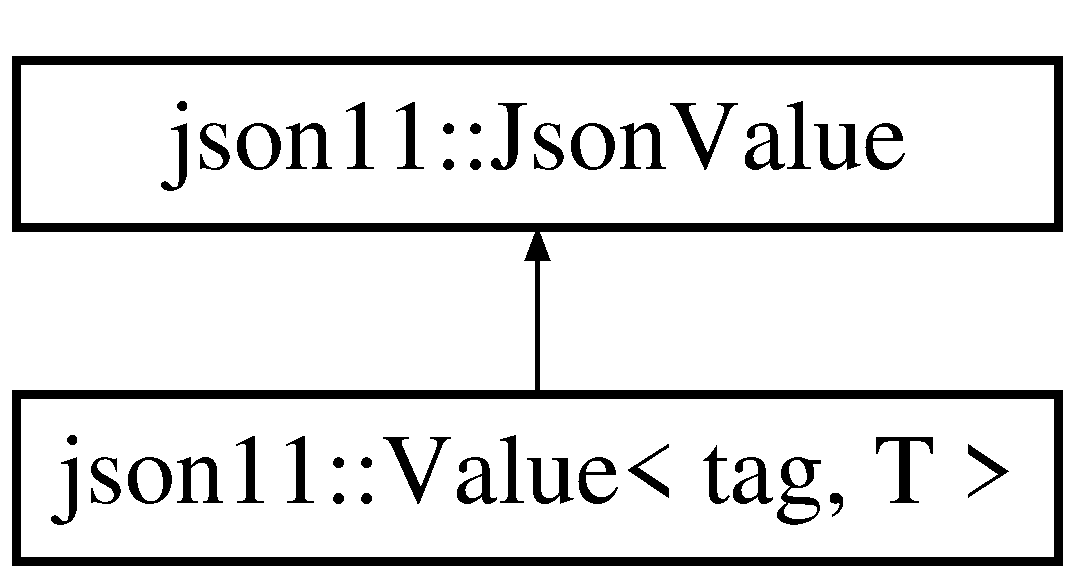
\includegraphics[height=2.000000cm]{classjson11_1_1_value}
\end{center}
\end{figure}
\subsection*{Protected Member Functions}
\begin{DoxyCompactItemize}
\item 
\mbox{\Hypertarget{classjson11_1_1_value_a0ba1c06e0de70655878b52ae47c9d876}\label{classjson11_1_1_value_a0ba1c06e0de70655878b52ae47c9d876}} 
{\bfseries Value} (const T \&value)
\item 
\mbox{\Hypertarget{classjson11_1_1_value_adf0aaa04f8f04d67cd45e7065270f21c}\label{classjson11_1_1_value_adf0aaa04f8f04d67cd45e7065270f21c}} 
{\bfseries Value} (T \&\&value)
\item 
\mbox{\Hypertarget{classjson11_1_1_value_a7f859afc6549e1616384c1ed8b95773e}\label{classjson11_1_1_value_a7f859afc6549e1616384c1ed8b95773e}} 
Json\+::\+Type {\bfseries type} () const override
\item 
\mbox{\Hypertarget{classjson11_1_1_value_a9e55dfa0c1119e102fd9bd9bb5bb1f56}\label{classjson11_1_1_value_a9e55dfa0c1119e102fd9bd9bb5bb1f56}} 
bool {\bfseries equals} (const \mbox{\hyperlink{classjson11_1_1_json_value}{Json\+Value}} $\ast$other) const override
\item 
\mbox{\Hypertarget{classjson11_1_1_value_a7ea36aadc76a335a6eaf4d44af154732}\label{classjson11_1_1_value_a7ea36aadc76a335a6eaf4d44af154732}} 
bool {\bfseries less} (const \mbox{\hyperlink{classjson11_1_1_json_value}{Json\+Value}} $\ast$other) const override
\item 
\mbox{\Hypertarget{classjson11_1_1_value_ac7c653a5479bb6f766e01a80bb06927f}\label{classjson11_1_1_value_ac7c653a5479bb6f766e01a80bb06927f}} 
void {\bfseries dump} (string \&out) const override
\end{DoxyCompactItemize}
\subsection*{Protected Attributes}
\begin{DoxyCompactItemize}
\item 
\mbox{\Hypertarget{classjson11_1_1_value_a248561db10925d05532a3c2b3ec5b916}\label{classjson11_1_1_value_a248561db10925d05532a3c2b3ec5b916}} 
const T {\bfseries m\+\_\+value}
\end{DoxyCompactItemize}


The documentation for this class was generated from the following file\+:\begin{DoxyCompactItemize}
\item 
/\+Users/h\+Gen/\+Desktop/qt/glwarp-\/configuration-\/tool/src/lib/json11.\+cpp\end{DoxyCompactItemize}

%--- End generated contents ---

% Index
\backmatter
\newpage
\phantomsection
\clearemptydoublepage
\addcontentsline{toc}{chapter}{Index}
\printindex

\end{document}
